\chapter{Control Plots}
\label{sec:CRplots}

Figures~\ref{fig:0bmu_zeroB_3_4jets_CR} to \ref{fig:0bele_0p5_CR} show distributions of observables in sidebands at low \njet, separately for electrons and muons.
Figures~\ref{fig:0bmu_zeroB_3_4jets_CR} and \ref{fig:0bele_zeroB_3_4jets_CR} present the sideband defined by $\LT>250\GeV$, $\HT>500\GeV$, and $3\leq\njet\leq4$, used in the estimation of the $\wJets$ background.
Figures~\ref{fig:0bmu_1B_4_5jets_CR} and \ref{fig:0bele_1B_4_5jets_CR} show the sideband defined by $\LT>250\GeV$, $\HT>500\GeV$, $\nbjet\geq1$, and $4\leq\njet\leq5$, used in the estimation of the $\ttJets$ background.
Distributions in the mainband are shown in Figures~\ref{fig:0bmu_0p5_CR} and \ref{fig:0bele_0p5_CR}.

\begin{figure}[p]
  \begin{center}
    \subfigure[\njet]{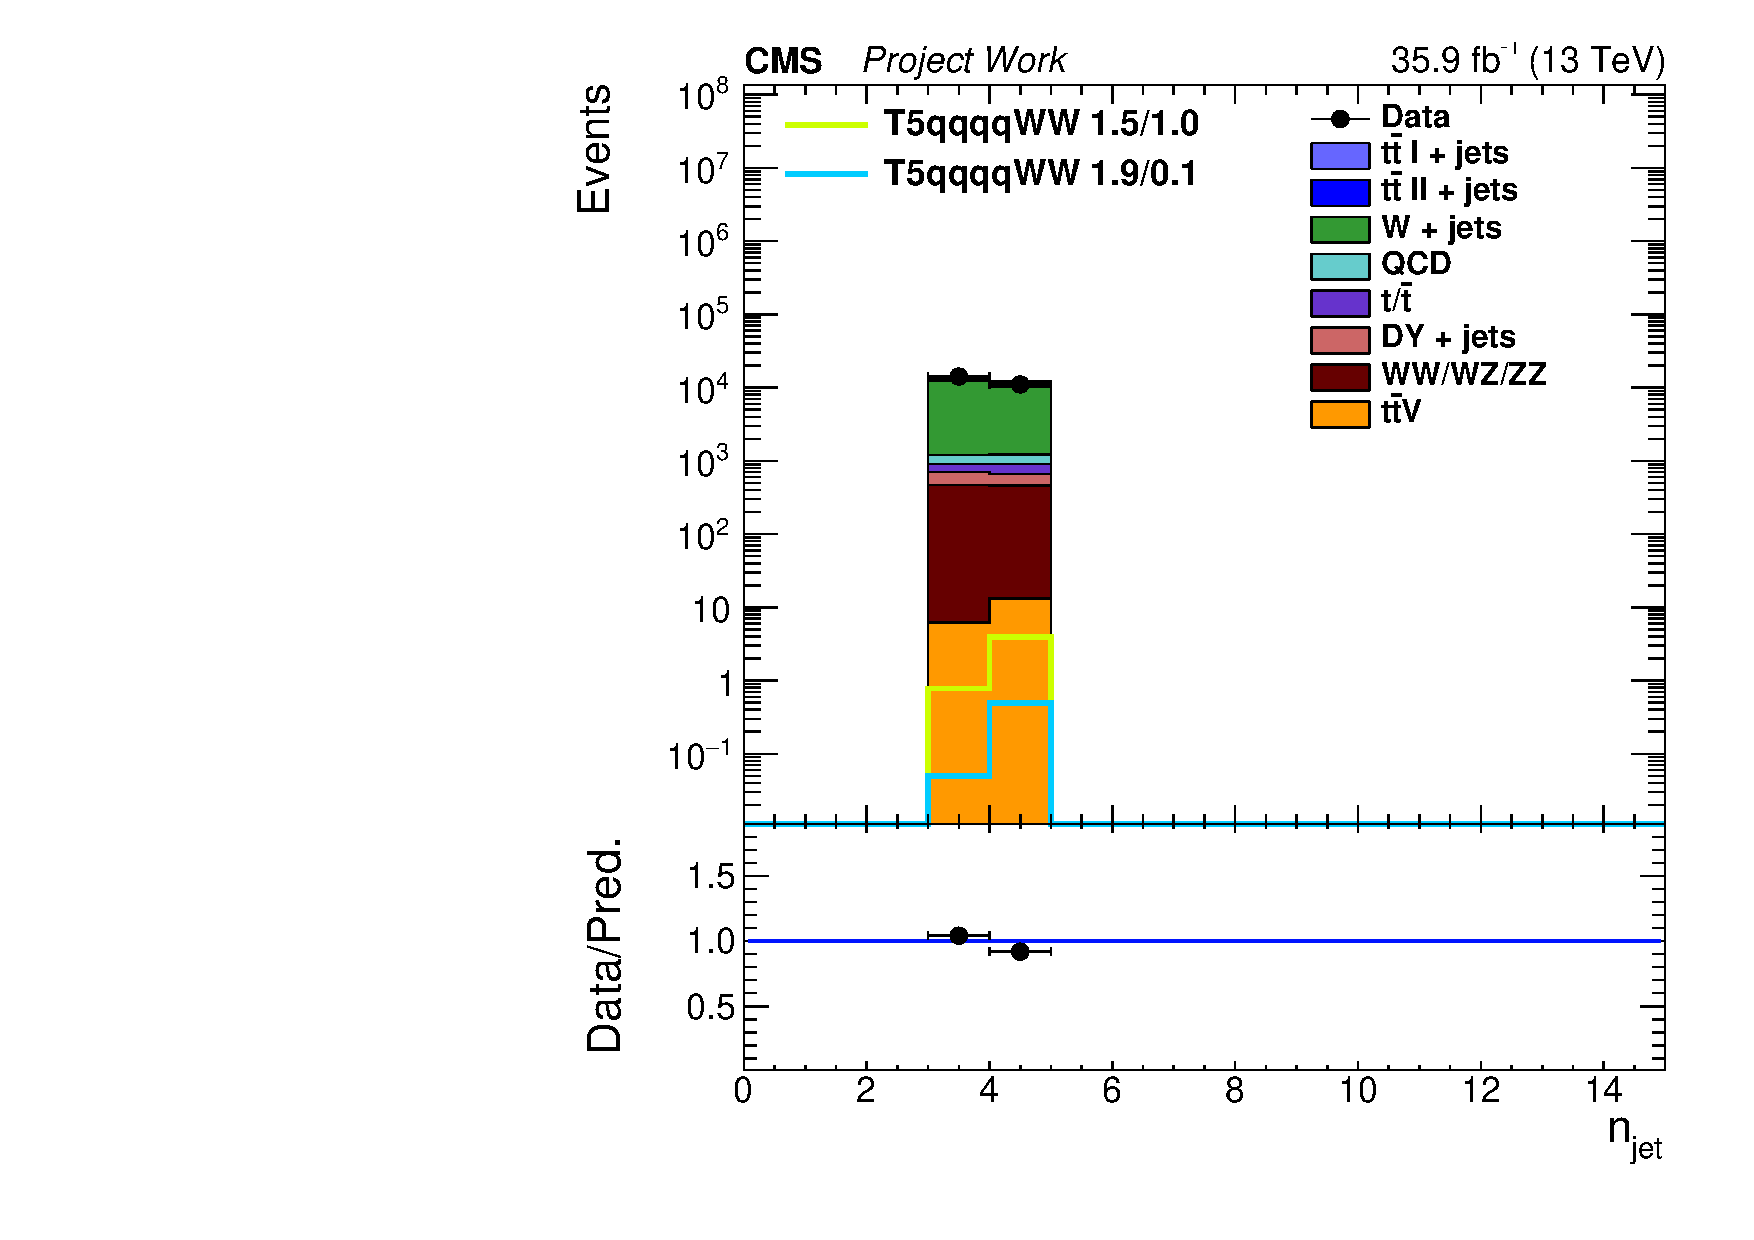
\includegraphics[angle=0,width=.32\textwidth]              {Plots//analysis/control_Plots/mu/st250_ht500_njet3-4_nbtagEq0/nJet30Project_Work.pdf}}
    \subfigure[$p_T(\textrm{1st jet})$]{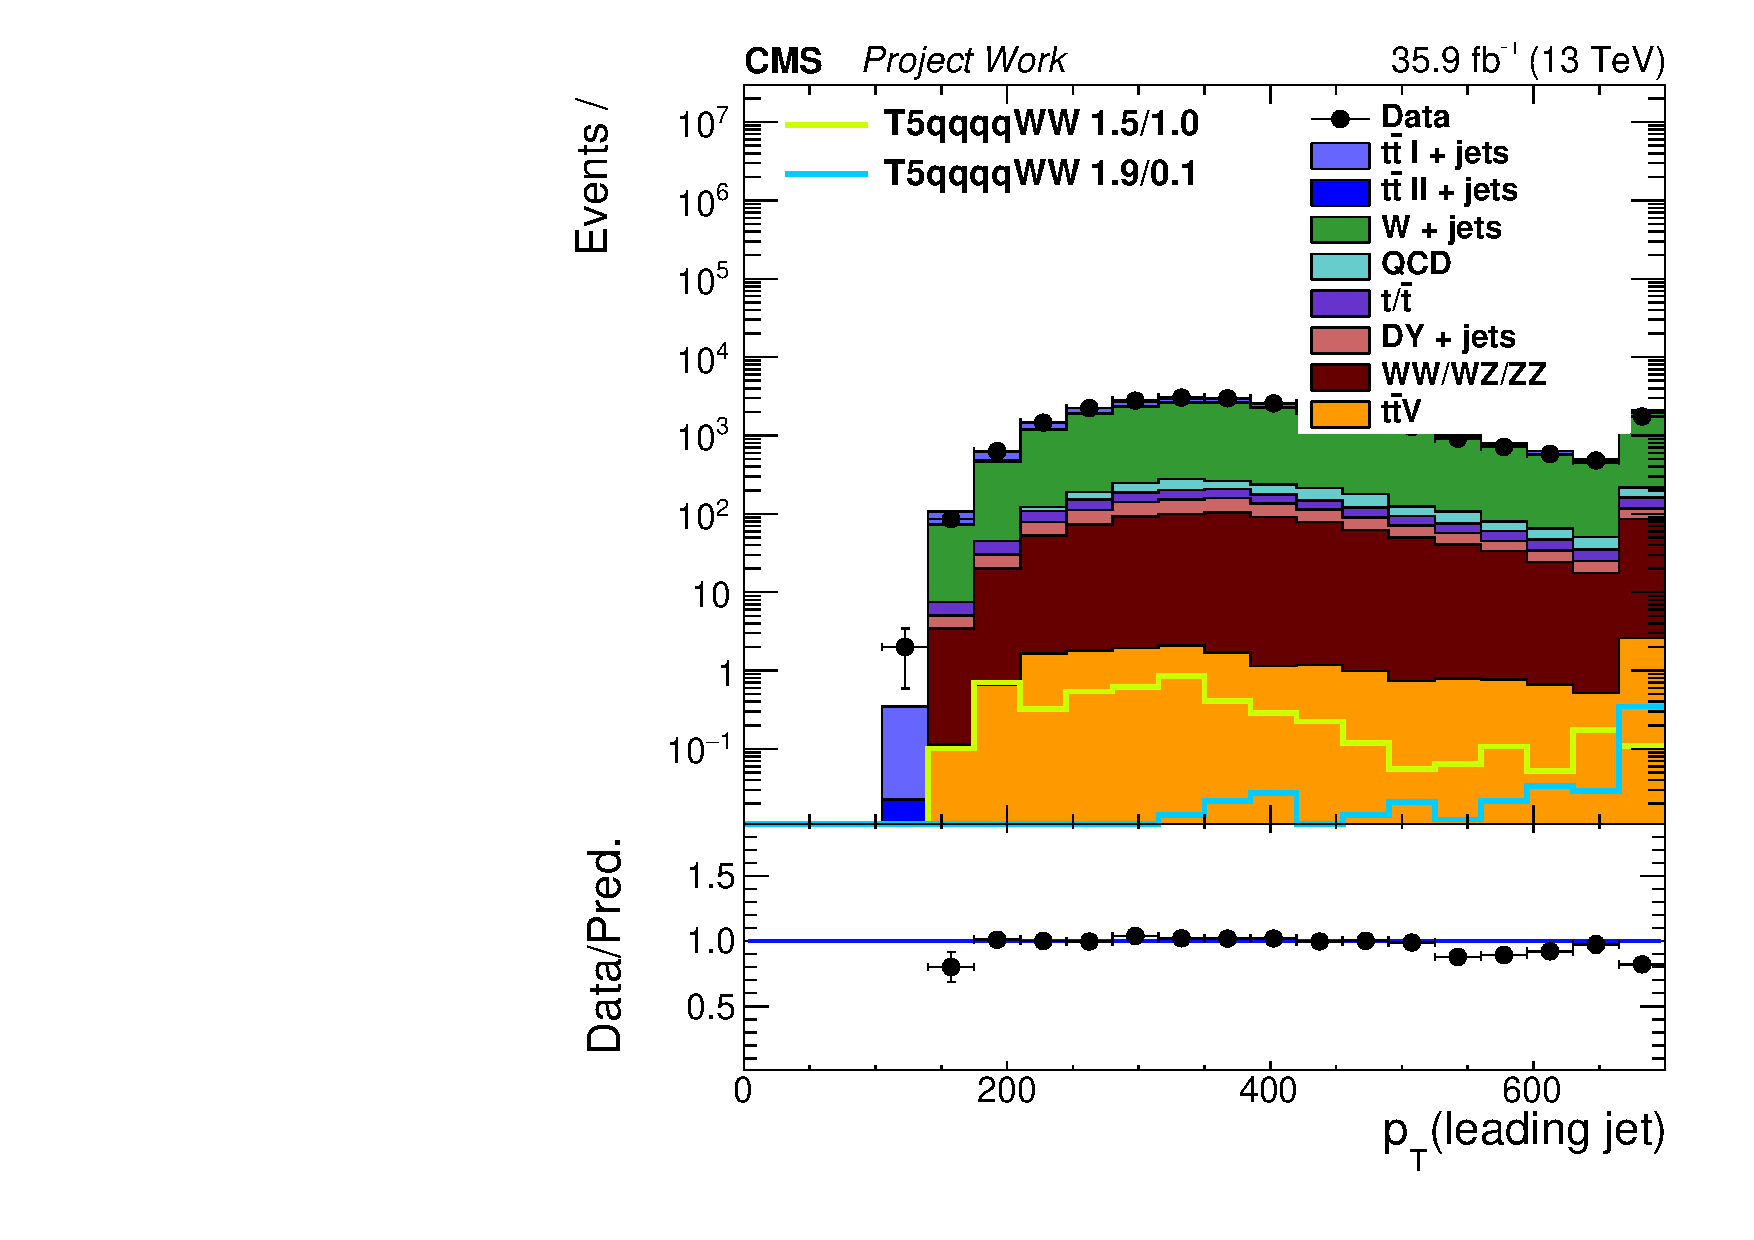
\includegraphics[angle=0,width=.32\textwidth]{Plots//analysis/control_Plots/mu/st250_ht500_njet3-4_nbtagEq0/leading_JetPtProject_Work.pdf}}
    \subfigure[$n_{\textrm{vertex}}$]{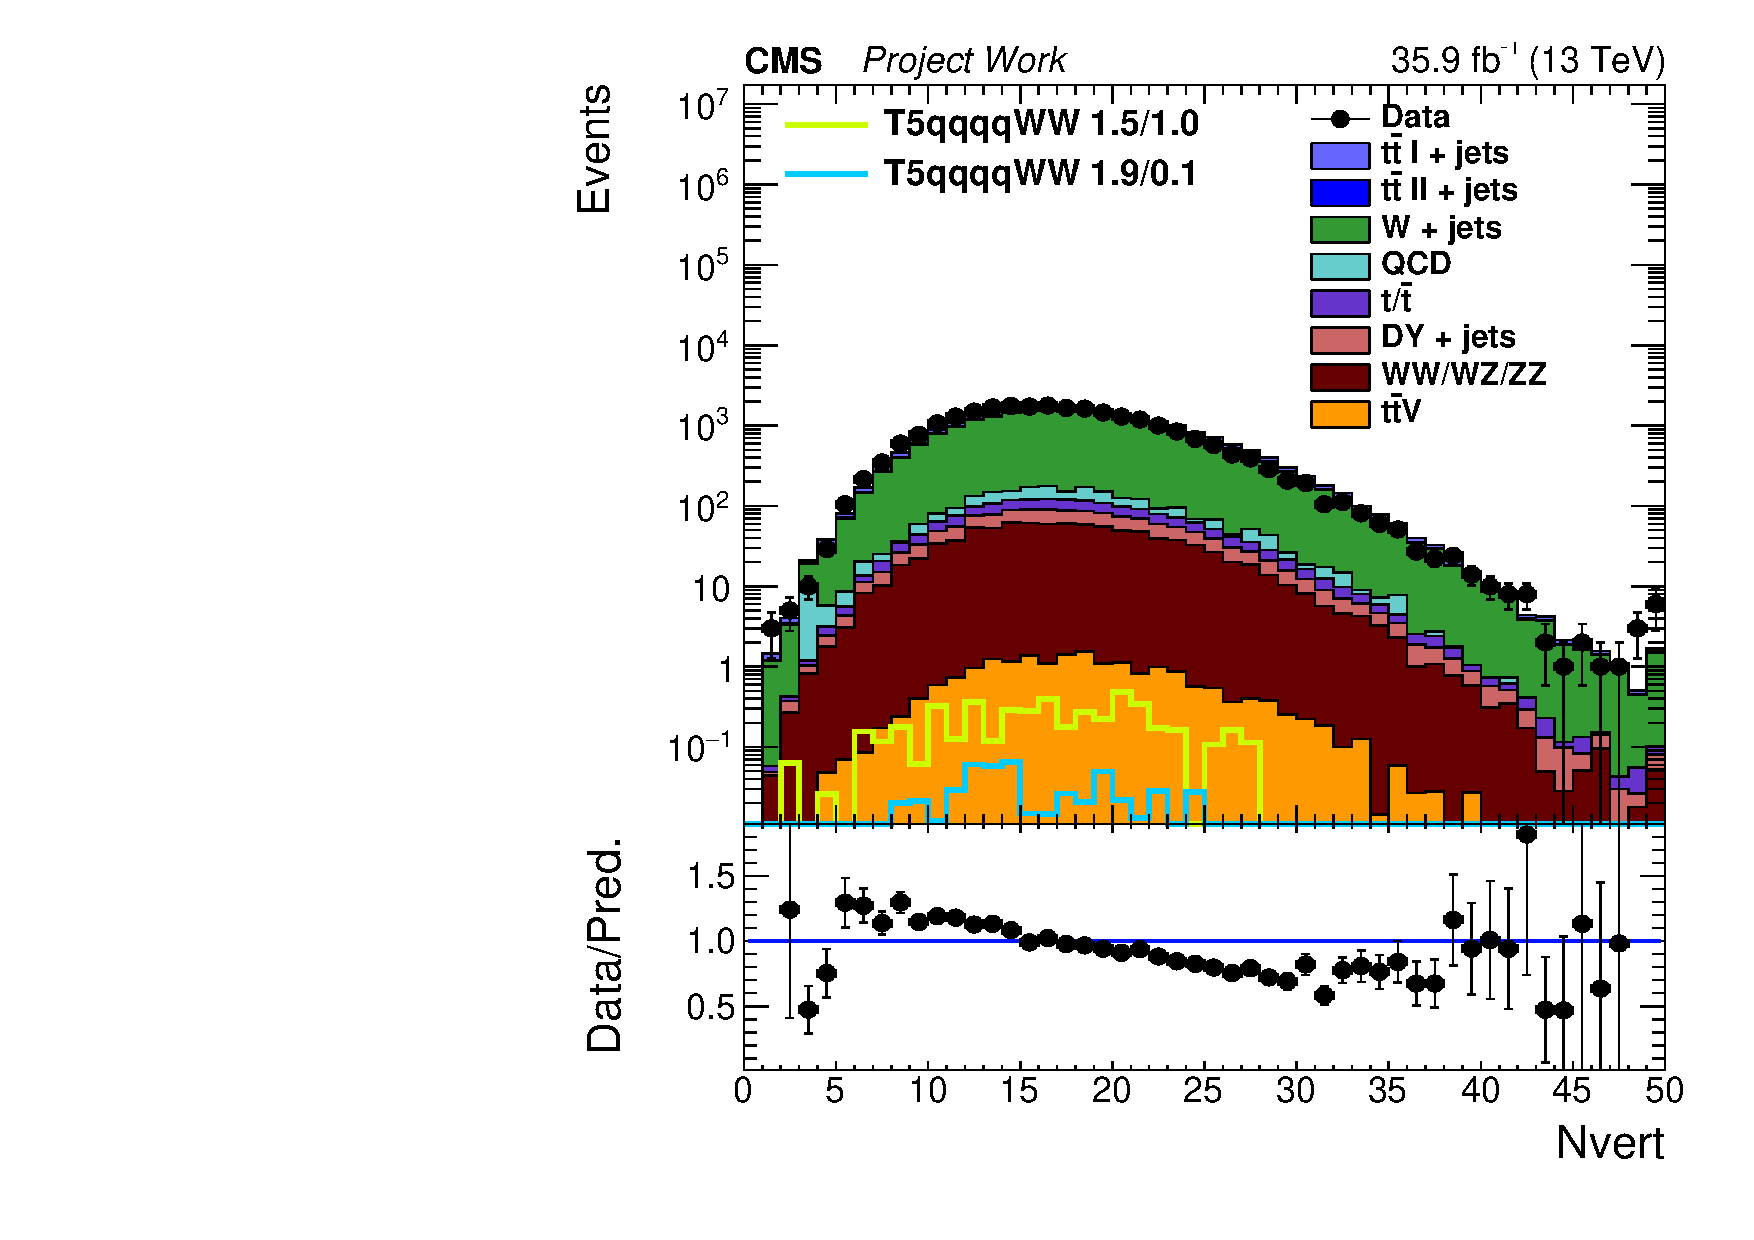
\includegraphics[angle=0,width=.32\textwidth]       {Plots//analysis/control_Plots/mu/st250_ht500_njet3-4_nbtagEq0/nVertProject_Work.pdf}}\\
    \subfigure[$p_T(l)$]{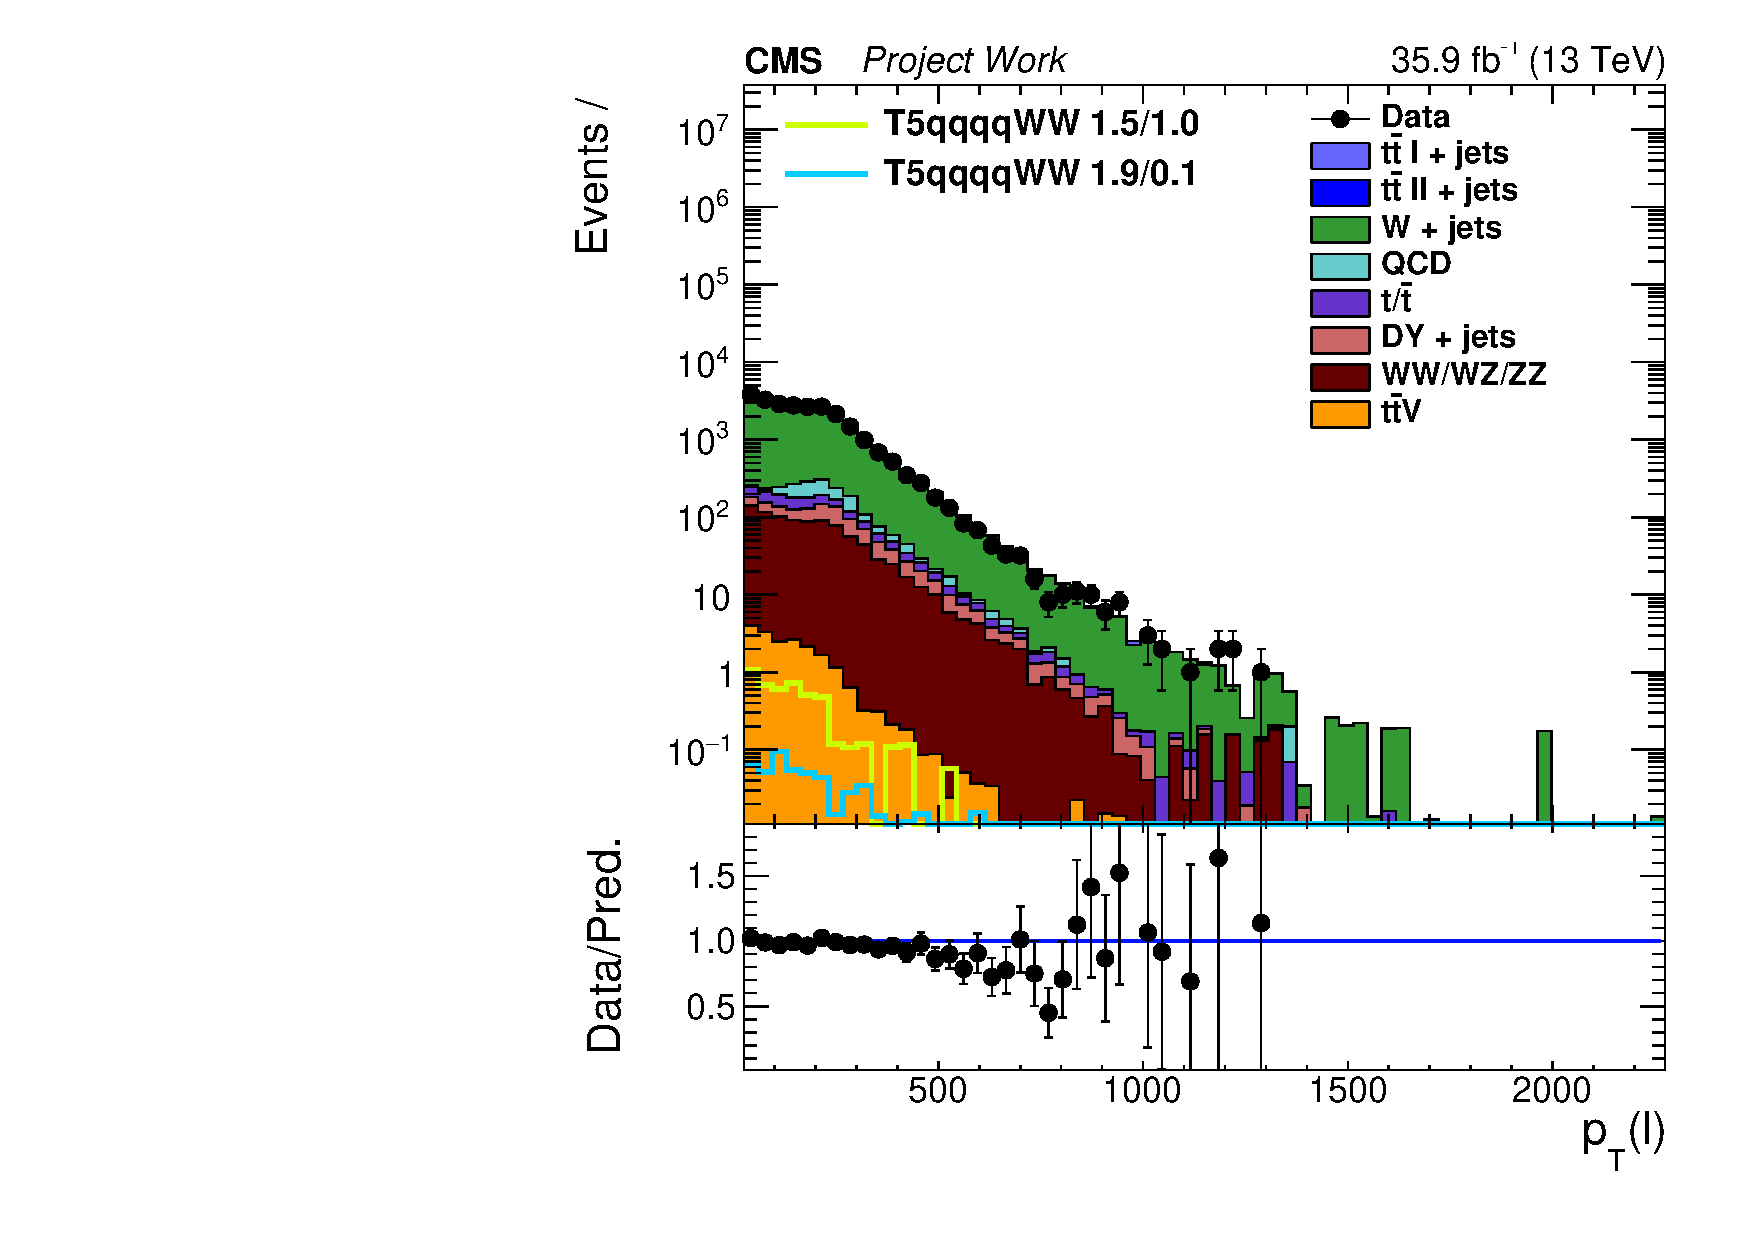
\includegraphics[angle=0,width=.32\textwidth]               {Plots//analysis/control_Plots/mu/st250_ht500_njet3-4_nbtagEq0/leptonPtProject_Work.pdf}}
    \subfigure[$m_{T2}$]{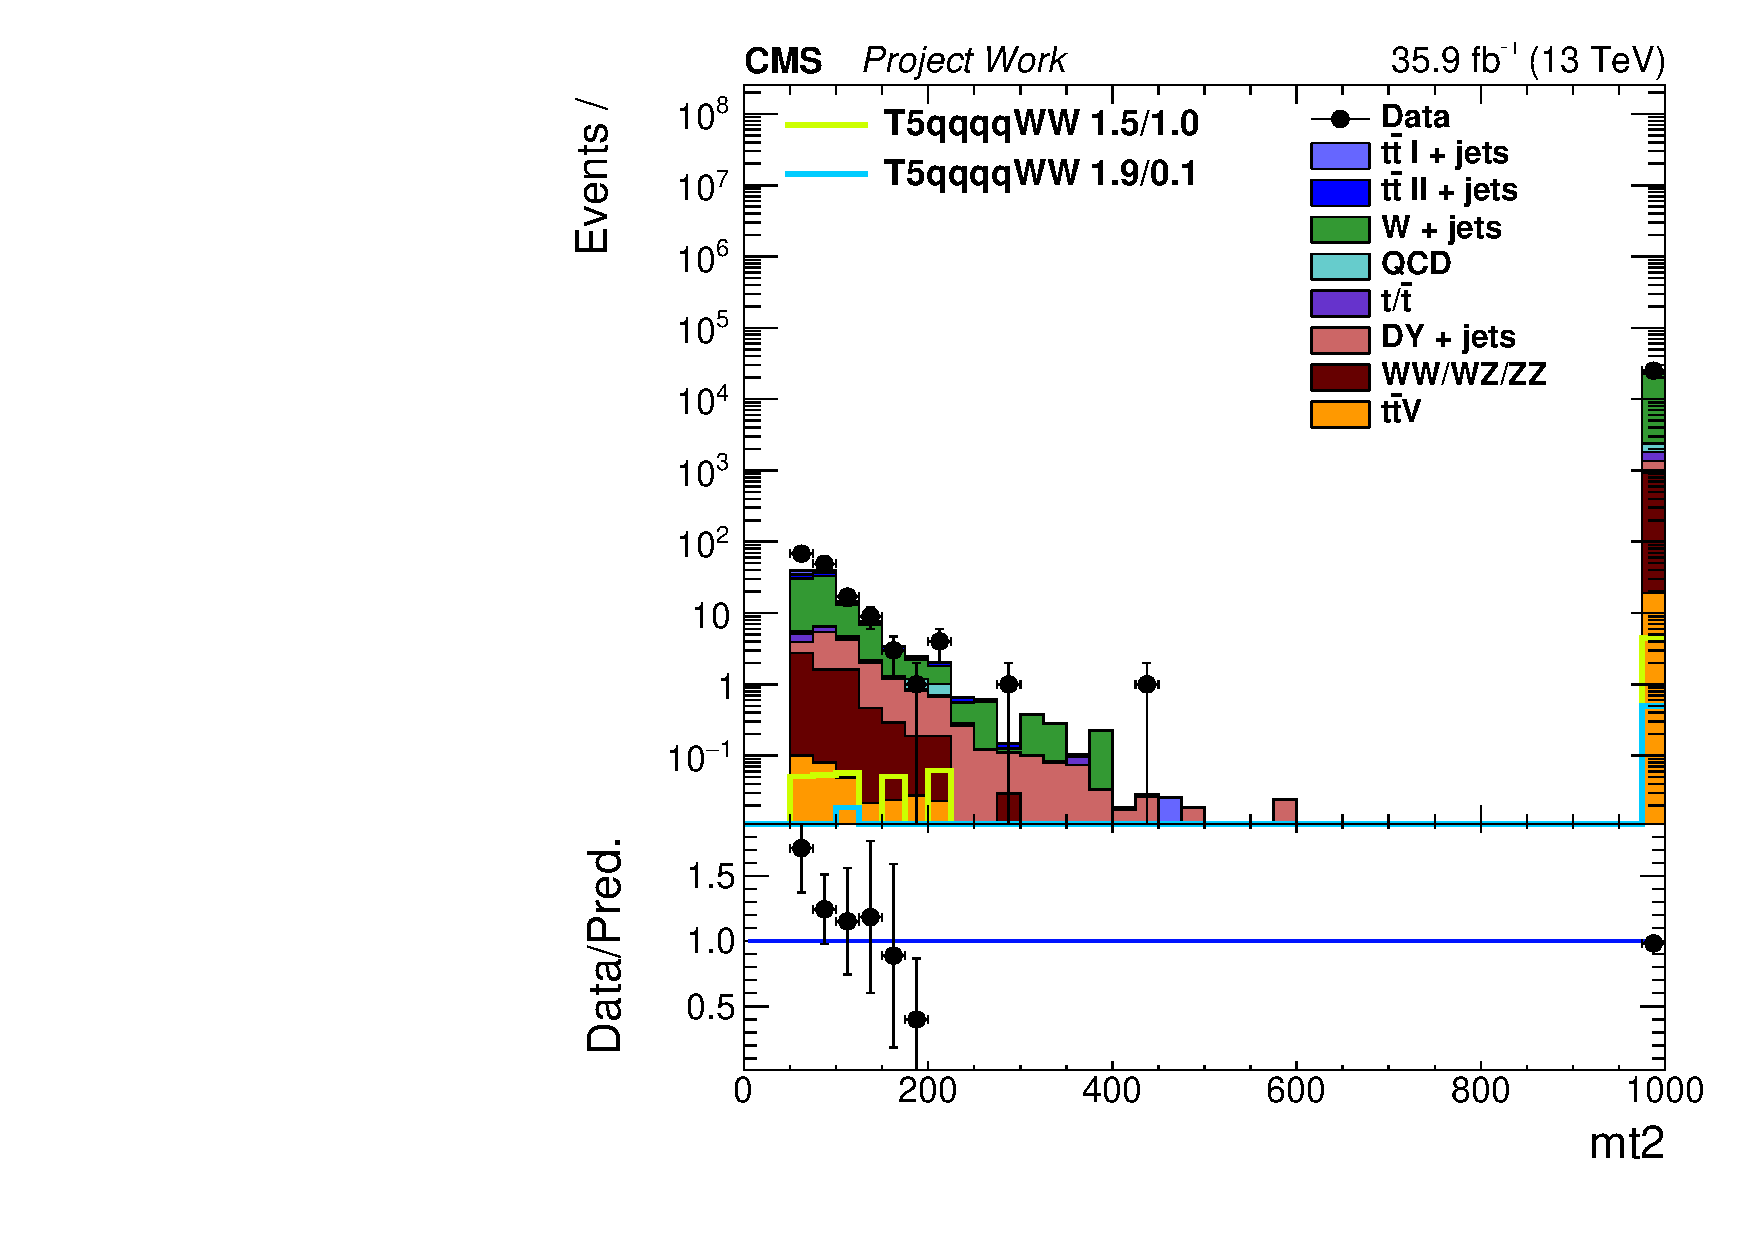
\includegraphics[angle=0,width=.32\textwidth]              {Plots//analysis/control_Plots/mu/st250_ht500_njet3-4_nbtagEq0/iso_MT2Project_Work.pdf}}
    \subfigure[miniIsolation$(l)$]{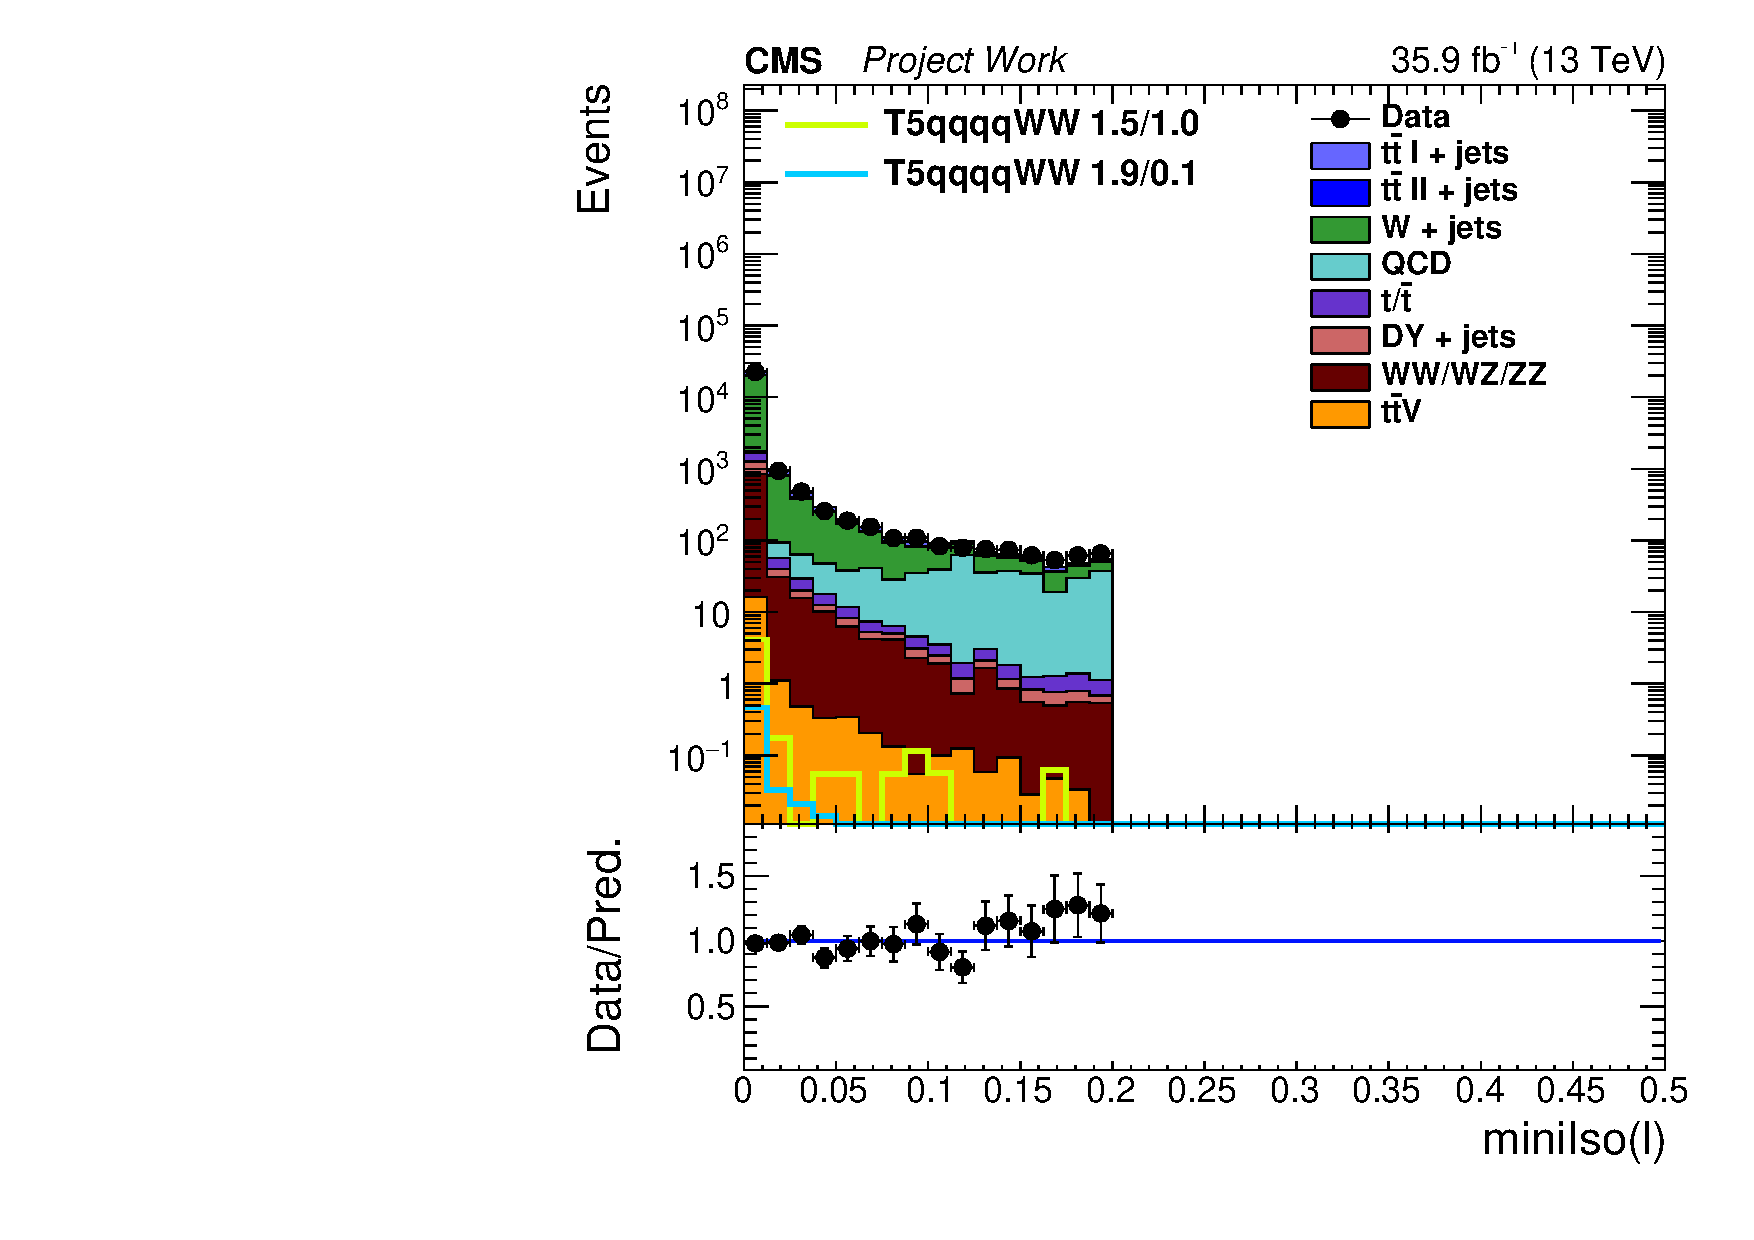
\includegraphics[angle=0,width=.32\textwidth]     {Plots//analysis/control_Plots/mu/st250_ht500_njet3-4_nbtagEq0/leptonminiIsoProject_Work.pdf}}\\
    \subfigure[\HT]{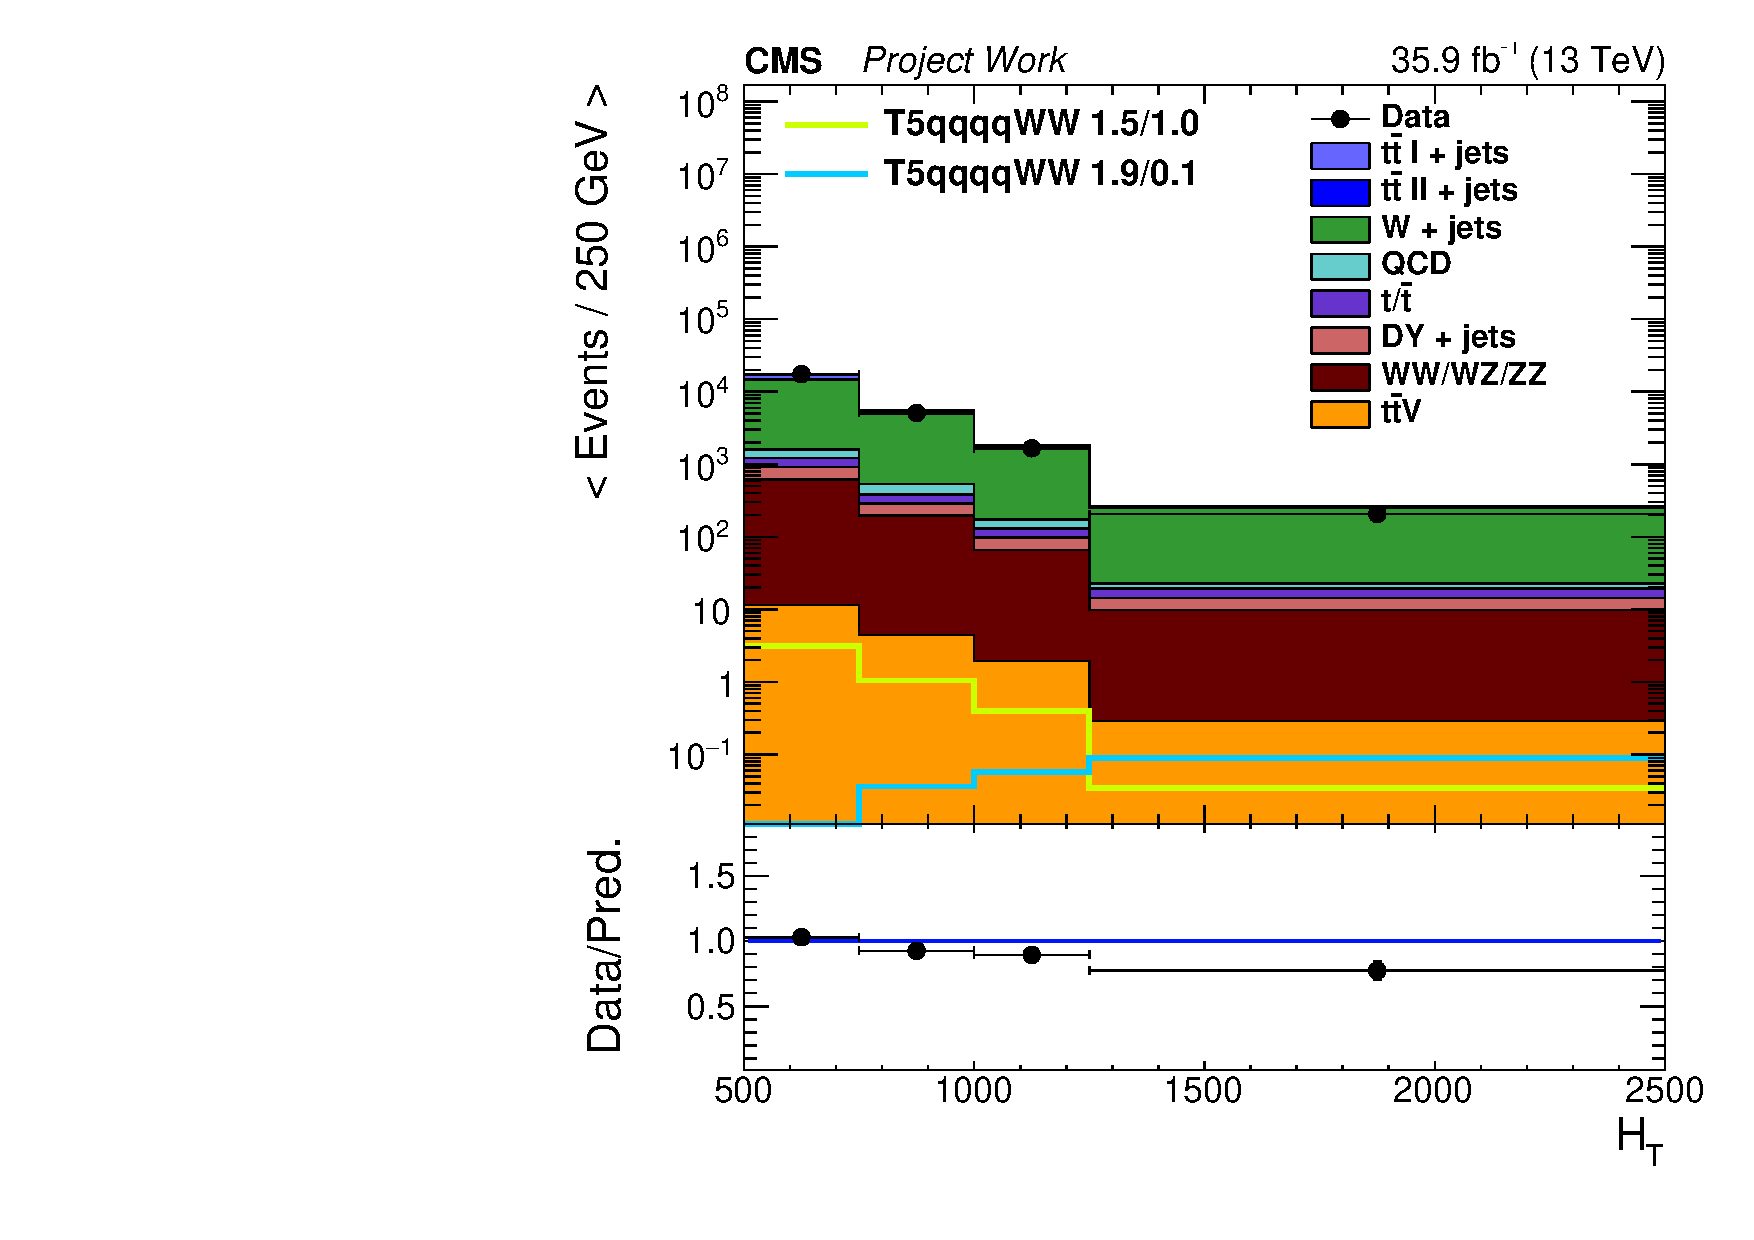
\includegraphics[angle=0,width=.32\textwidth]                    {Plots//analysis/control_Plots/mu/st250_ht500_njet3-4_nbtagEq0/htJet30jProject_Work.pdf}}
    \subfigure[\LT]{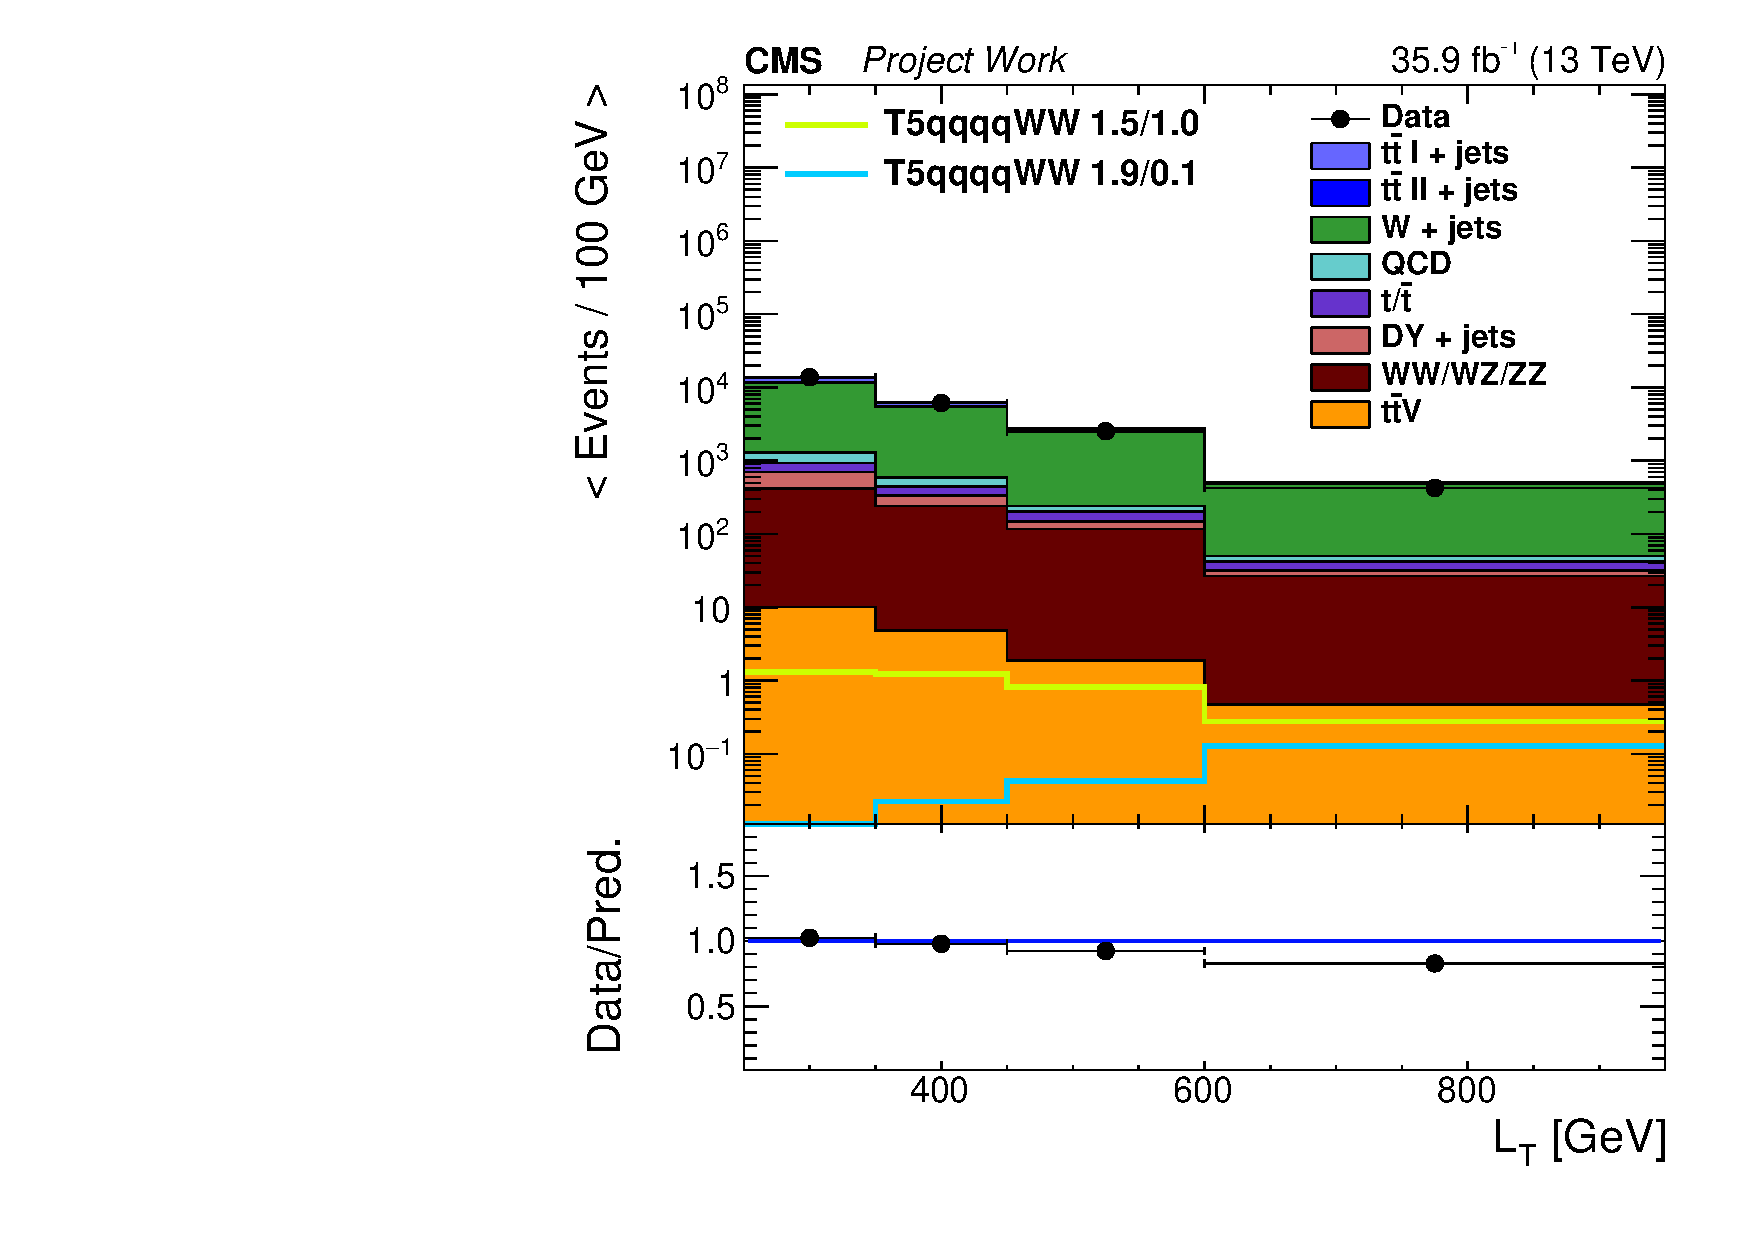
\includegraphics[angle=0,width=.32\textwidth]                    {Plots//analysis/control_Plots/mu/st250_ht500_njet3-4_nbtagEq0/LTProject_Work.pdf}}
    \subfigure[\DF]{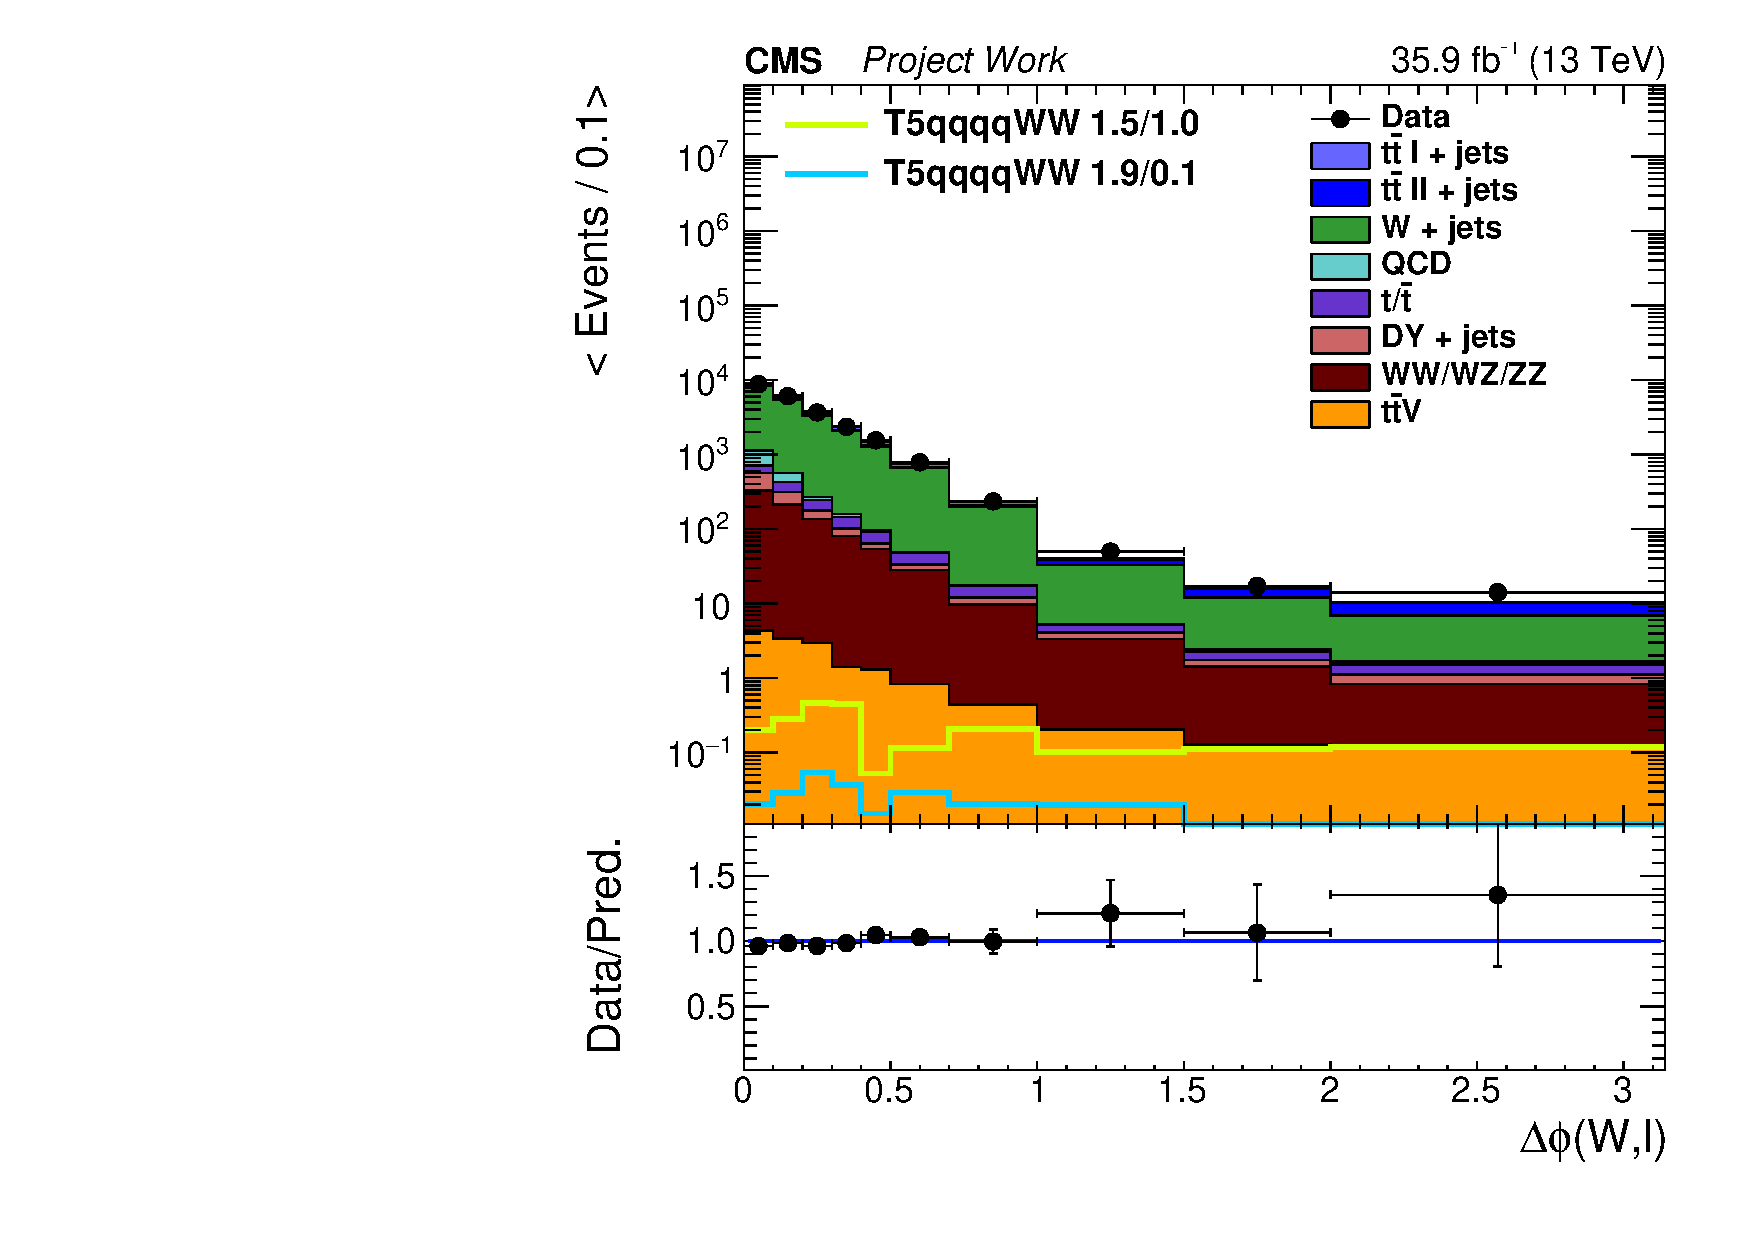
\includegraphics[angle=0,width=.32\textwidth]                    {Plots//analysis/control_Plots/mu/st250_ht500_njet3-4_nbtagEq0/deltaPhi_Wl_wideProject_Work.pdf}}

    \caption{Distribution of kinematic observables after requiring $\HT >$~500~\GeV, $\LT >$~250~\GeV, $3\leq$ jets $\leq4$  and zero b-tagged jets (1 $\mu$ channel).
      %In order to blind the signal region, data events with large \DF (corresponding to the dynamic \DF cut) are excluded from the \DF plot.
    }
    \label{fig:0bmu_zeroB_3_4jets_CR}
  \end{center}
\end{figure}

\begin{figure}[p]
  \begin{center}
    \subfigure[\njet]{\includegraphics[angle=0,width=.32\textwidth]                  {Plots//analysis/control_Plots/ele/st250_ht500_njet3-4_nbtagEq0/nJet30Project_Work.pdf}}
    \subfigure[$p_T(\textrm{1st jet})$]{\includegraphics[angle=0,width=.32\textwidth]{Plots//analysis/control_Plots/ele/st250_ht500_njet3-4_nbtagEq0/leading_JetPtProject_Work.pdf}}
    \subfigure[$n_{\textrm{vertex}}$]{\includegraphics[angle=0,width=.32\textwidth]       {Plots//analysis/control_Plots/ele/st250_ht500_njet3-4_nbtagEq0/nVertProject_Work.pdf}}\\
    \subfigure[$p_T(l)$]{\includegraphics[angle=0,width=.32\textwidth]               {Plots//analysis/control_Plots/ele/st250_ht500_njet3-4_nbtagEq0/leptonPtProject_Work.pdf}}
    \subfigure[$m_{T2}$]{\includegraphics[angle=0,width=.32\textwidth]              {Plots//analysis/control_Plots/ele/st250_ht500_njet3-4_nbtagEq0/iso_MT2Project_Work.pdf}}
    \subfigure[miniIsolation$(l)$]{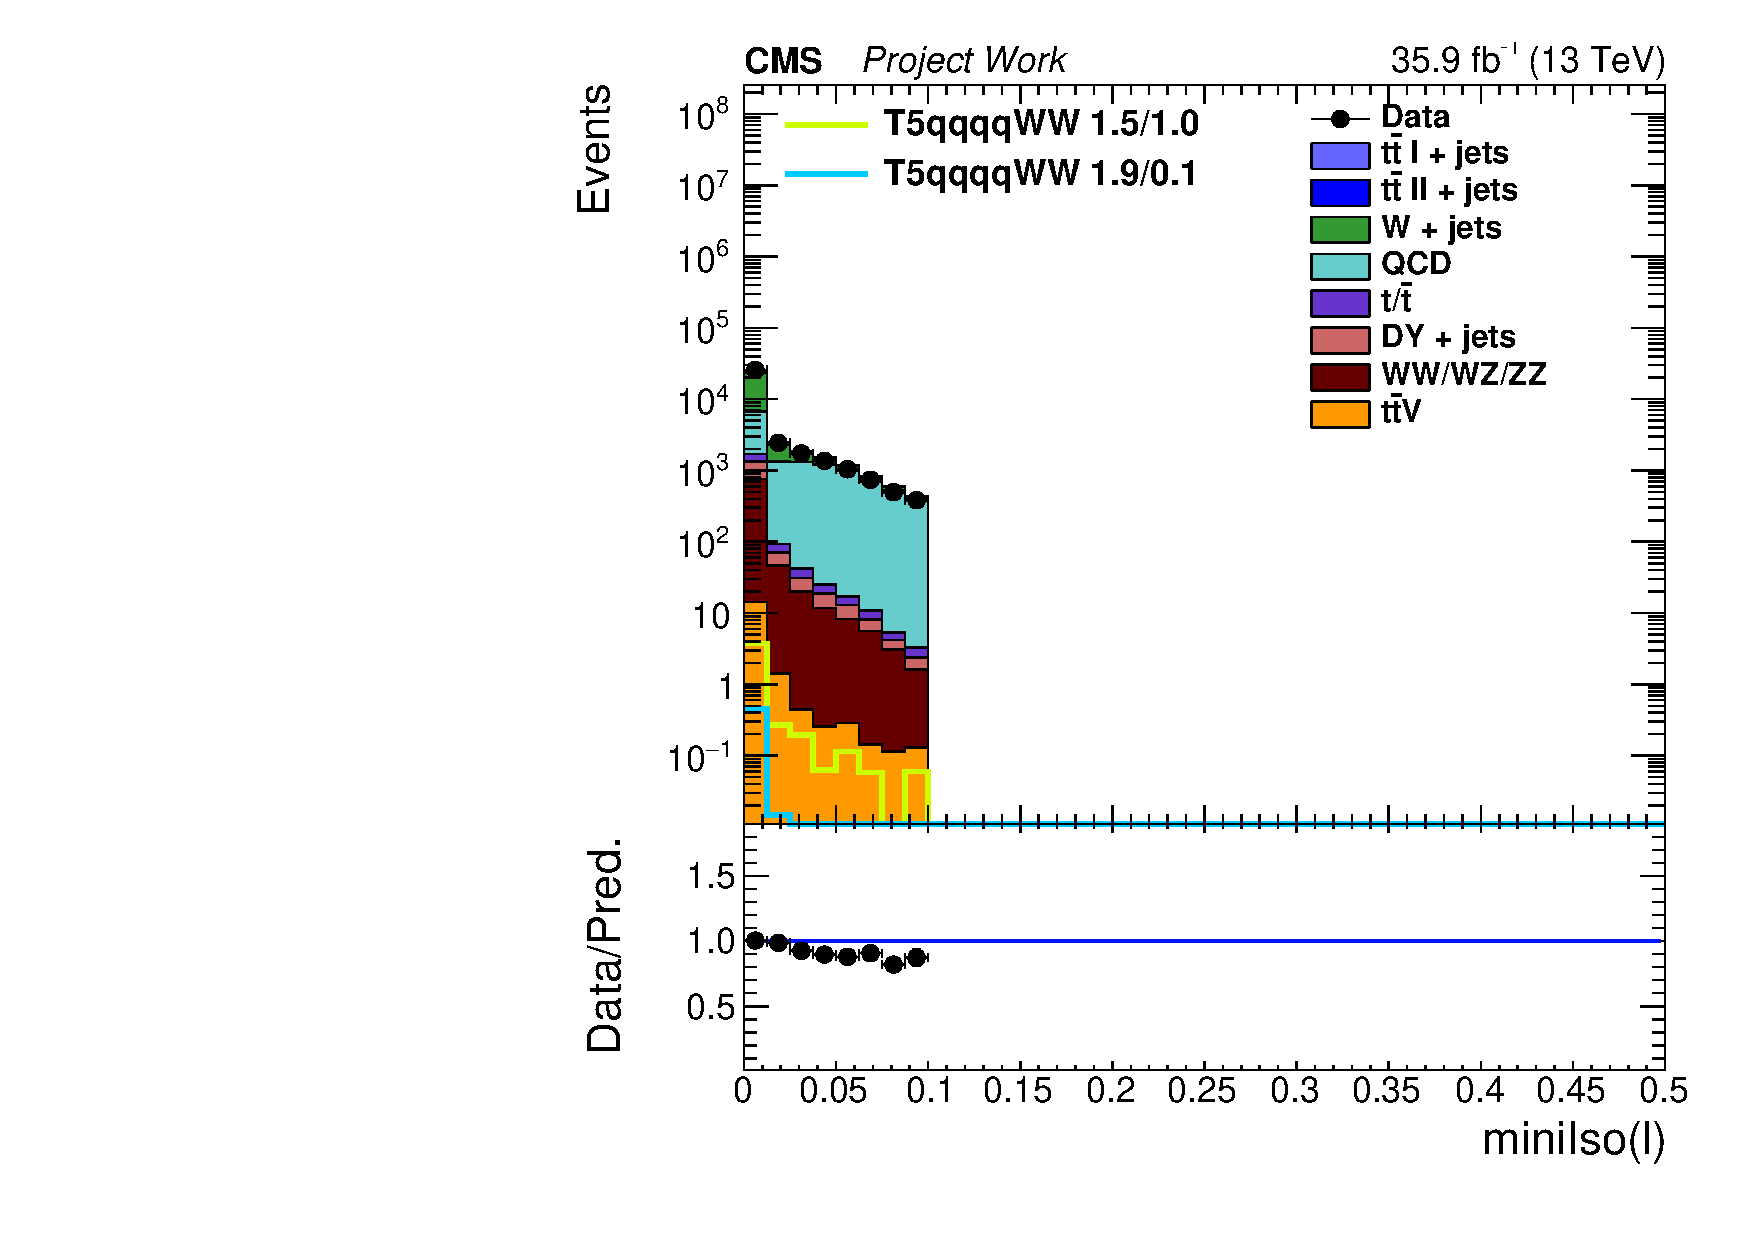
\includegraphics[angle=0,width=.32\textwidth]     {Plots//analysis/control_Plots/ele/st250_ht500_njet3-4_nbtagEq0/leptonminiIsoProject_Work.pdf}}\\
    \subfigure[\HT]{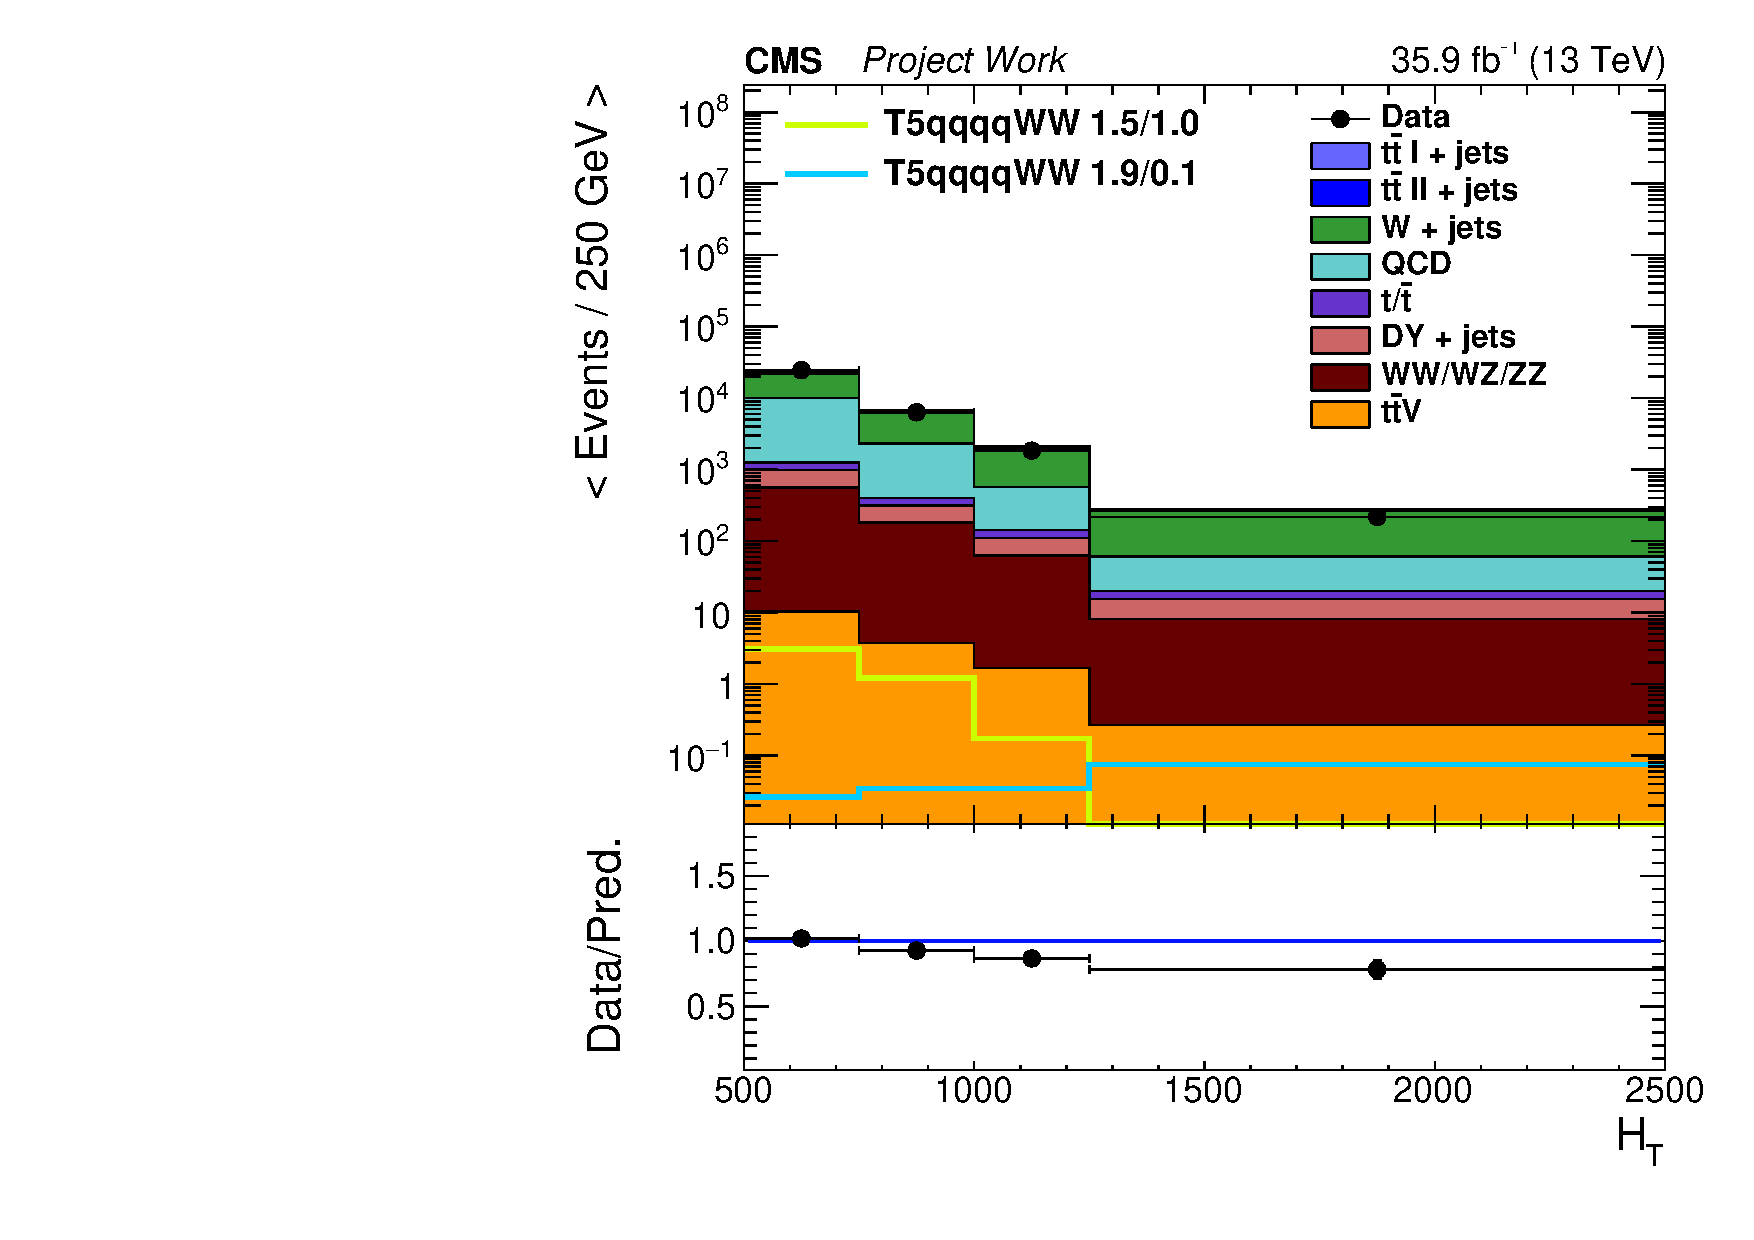
\includegraphics[angle=0,width=.32\textwidth]                    {Plots//analysis/control_Plots/ele/st250_ht500_njet3-4_nbtagEq0/htJet30jProject_Work.pdf}}
    \subfigure[\LT]{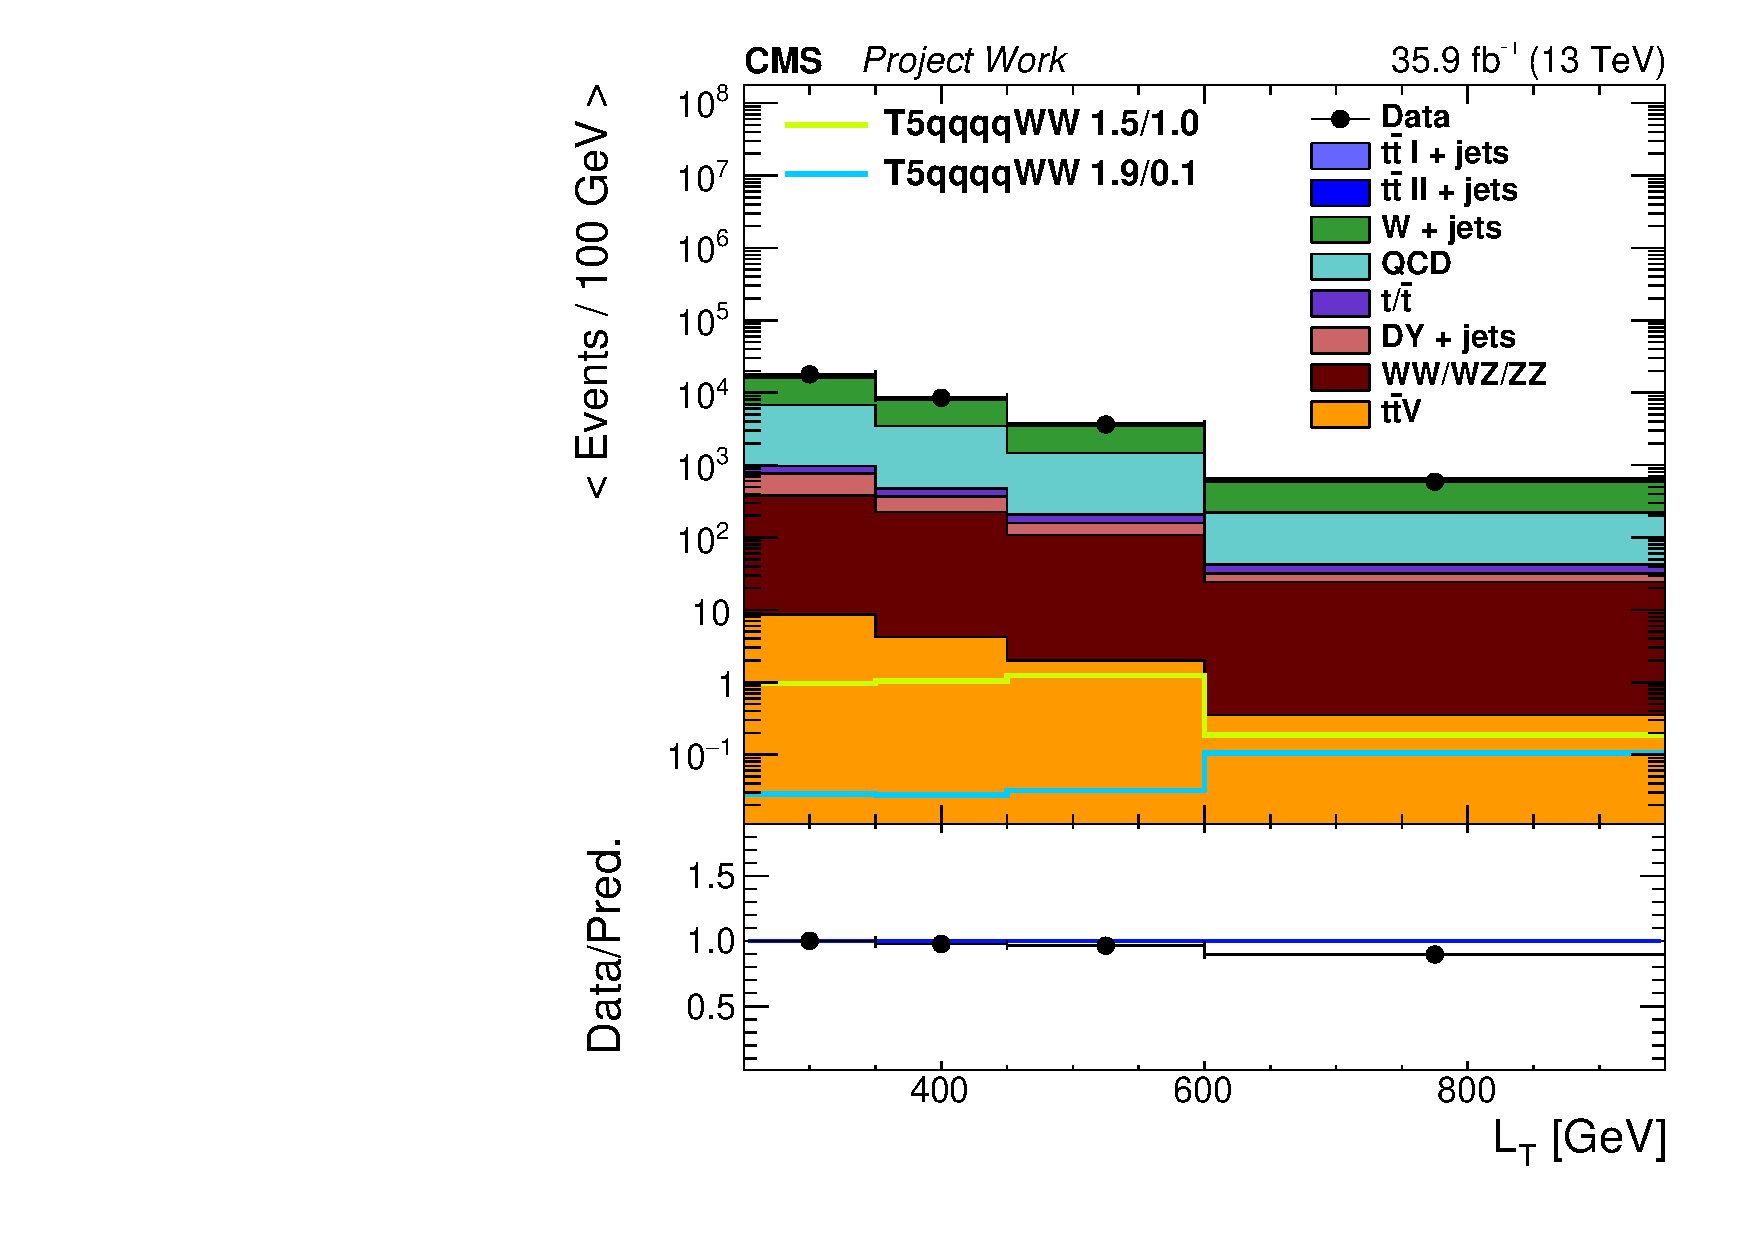
\includegraphics[angle=0,width=.32\textwidth]                    {Plots//analysis/control_Plots/ele/st250_ht500_njet3-4_nbtagEq0/LTProject_Work.pdf}}
    \subfigure[\DF]{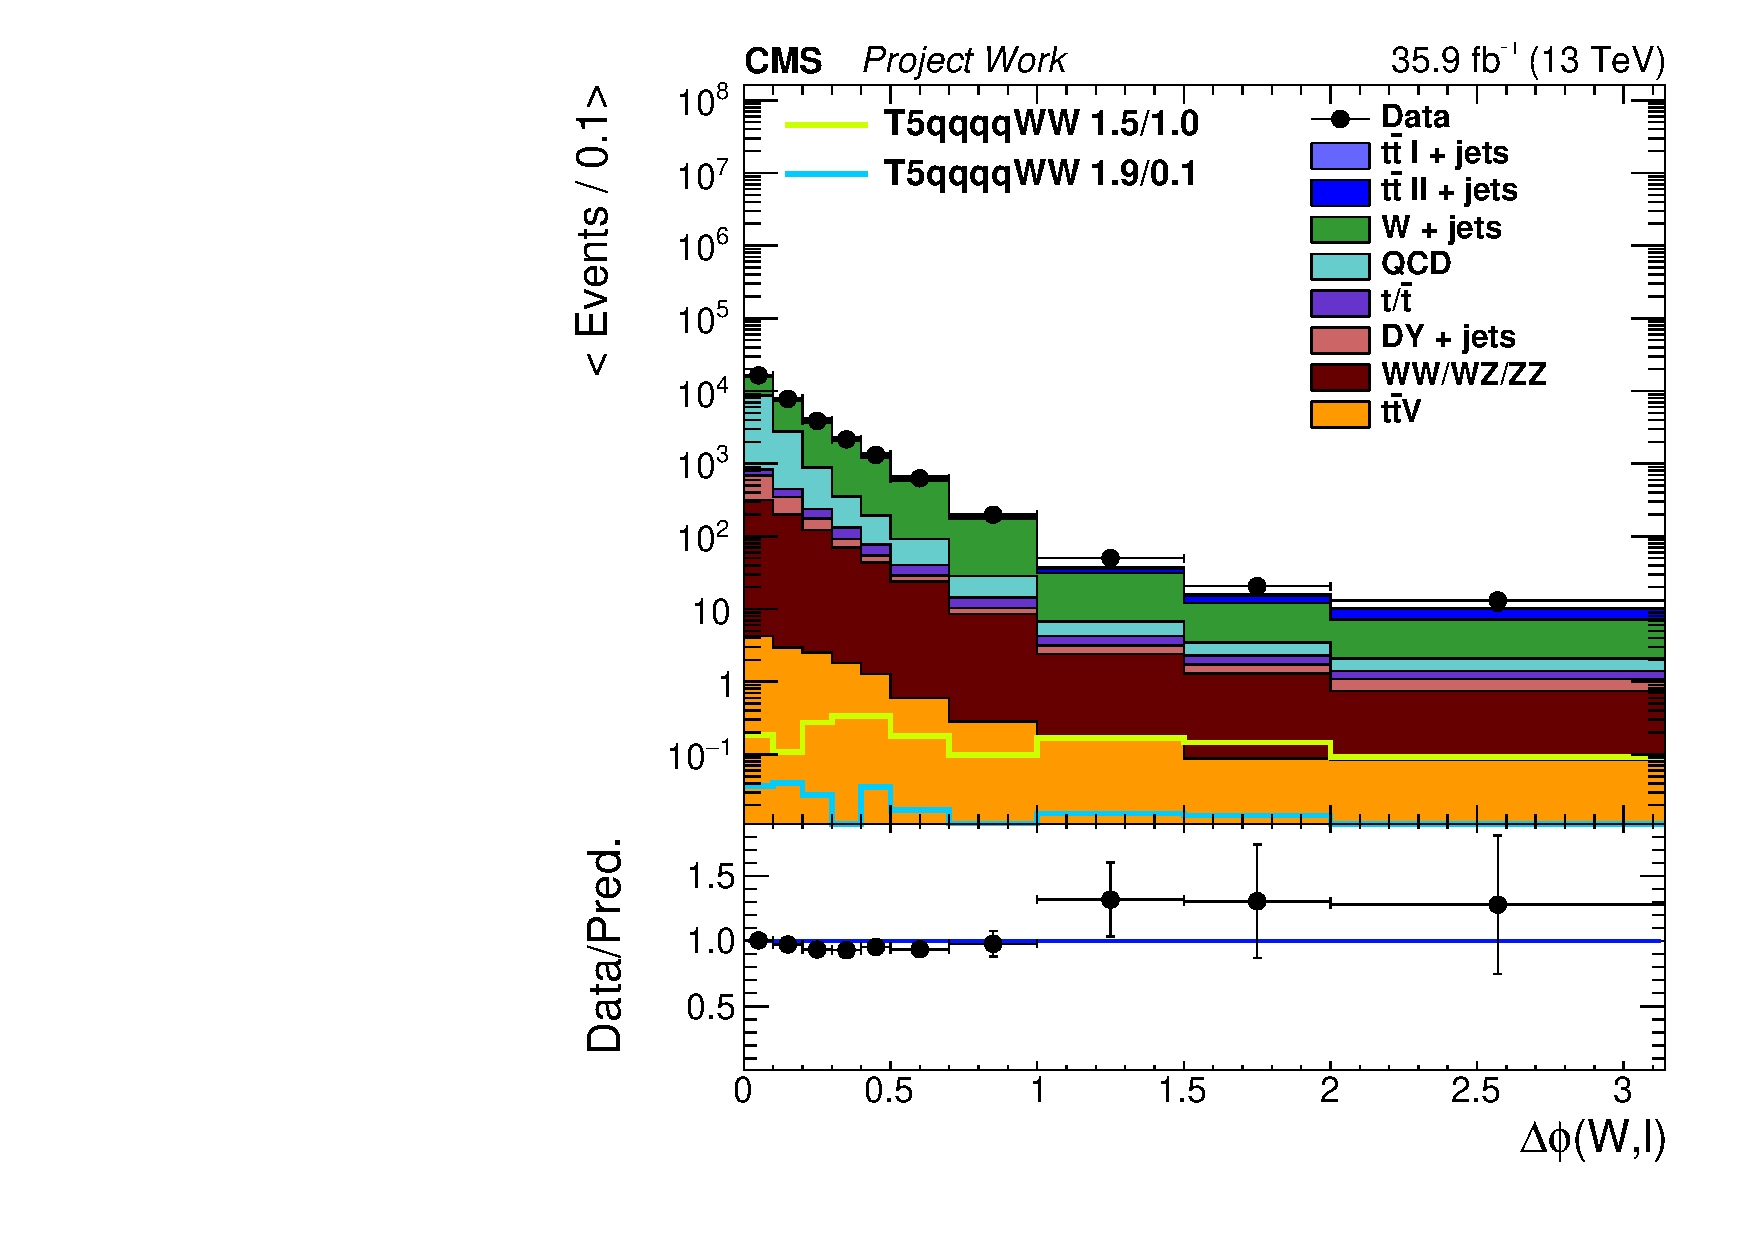
\includegraphics[angle=0,width=.32\textwidth]                    {Plots//analysis/control_Plots/ele/st250_ht500_njet3-4_nbtagEq0/deltaPhi_Wl_wideProject_Work.pdf}}

    \caption{Distribution of kinematic observables after requiring $\HT >$~500~\GeV, $\LT >$~250~\GeV, $3\leq$ jets $\leq4$  and zero b-tagged jets (1 $e$ channel).
      %In order to blind the signal region, data events with large \DF (corresponding to the dynamic \DF cut) are excluded from the \DF plot.
    }
    \label{fig:0bele_zeroB_3_4jets_CR}
  \end{center}
\end{figure}


\begin{figure}[p]
  \begin{center}
    \subfigure[\njet]{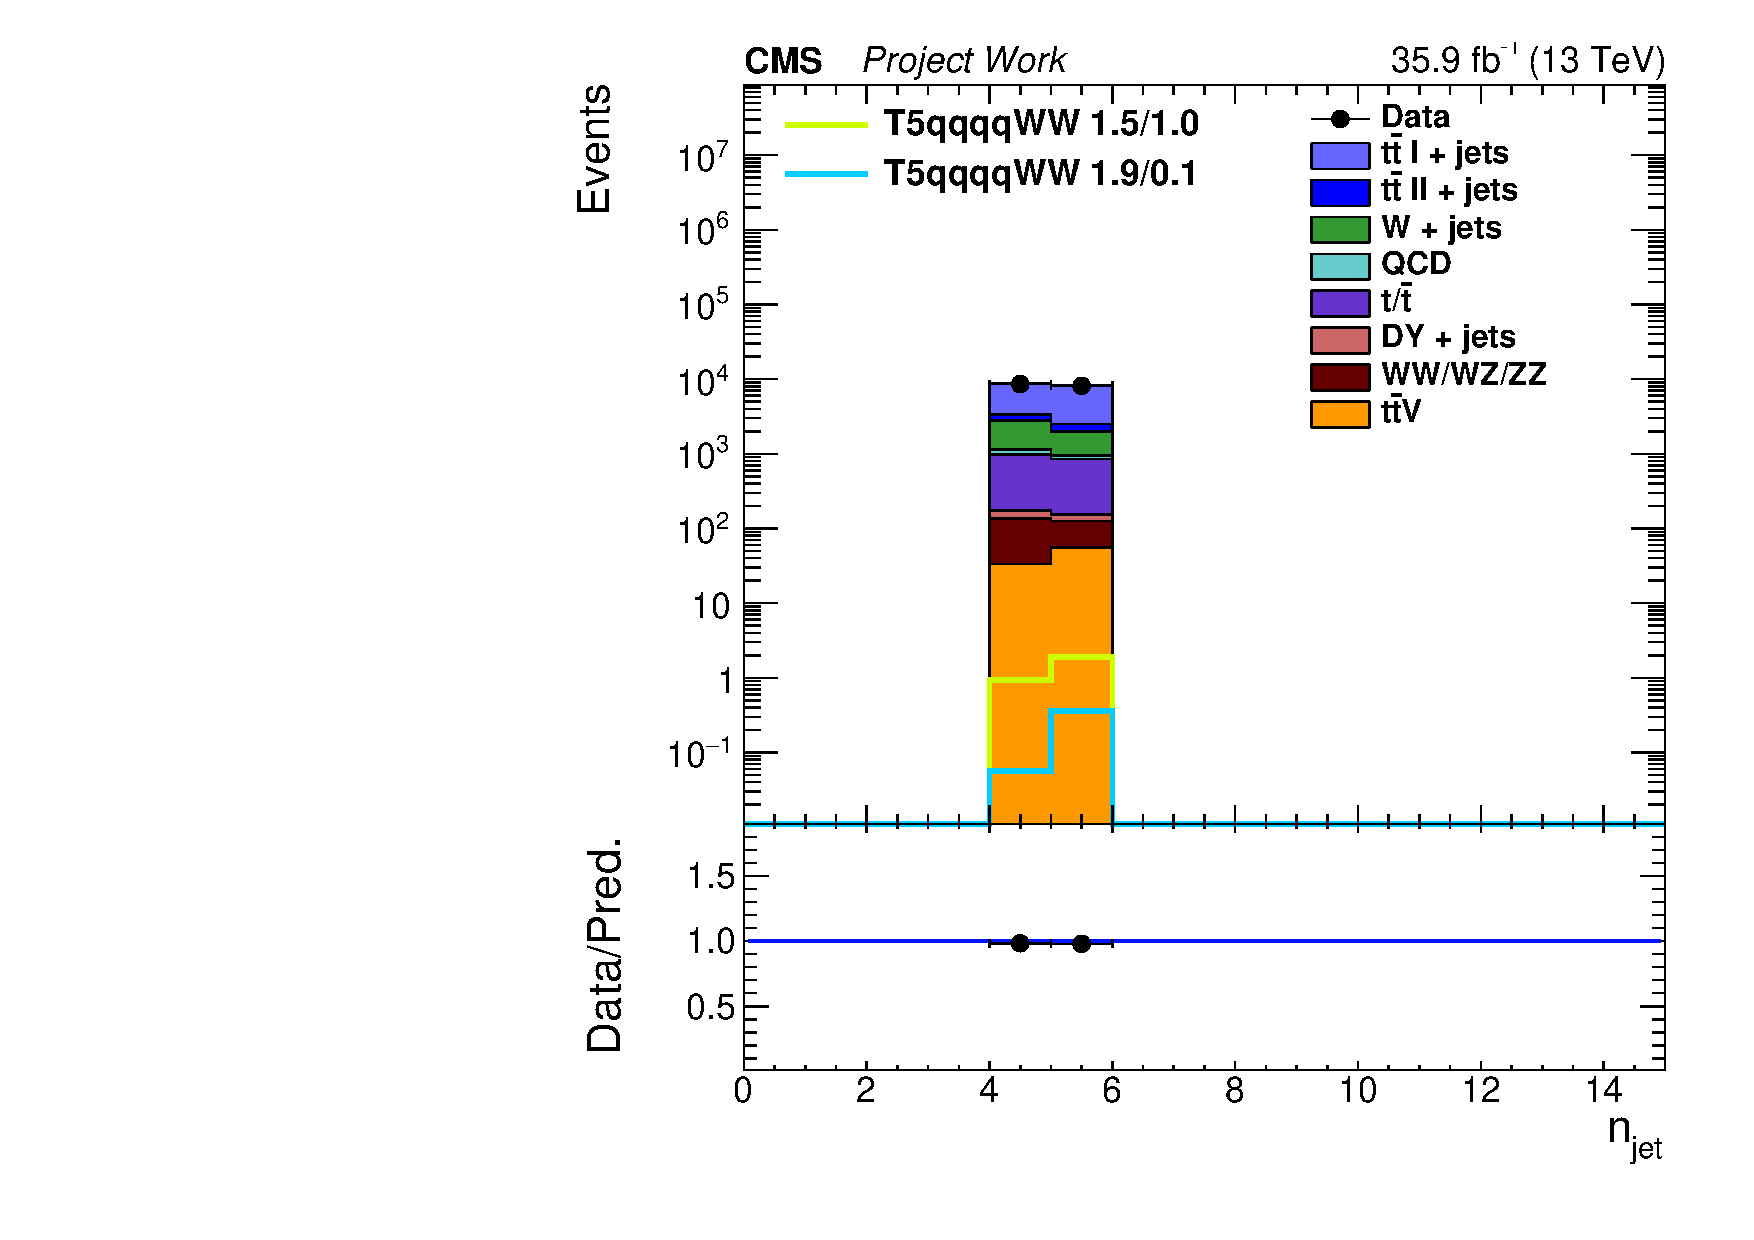
\includegraphics[angle=0,width=.32\textwidth]                  {Plots//analysis/control_Plots/mu/st250_ht500_njet4-5_nbtag1/nJet30Project_Work.pdf}}
    \subfigure[$p_T(\textrm{1st jet})$]{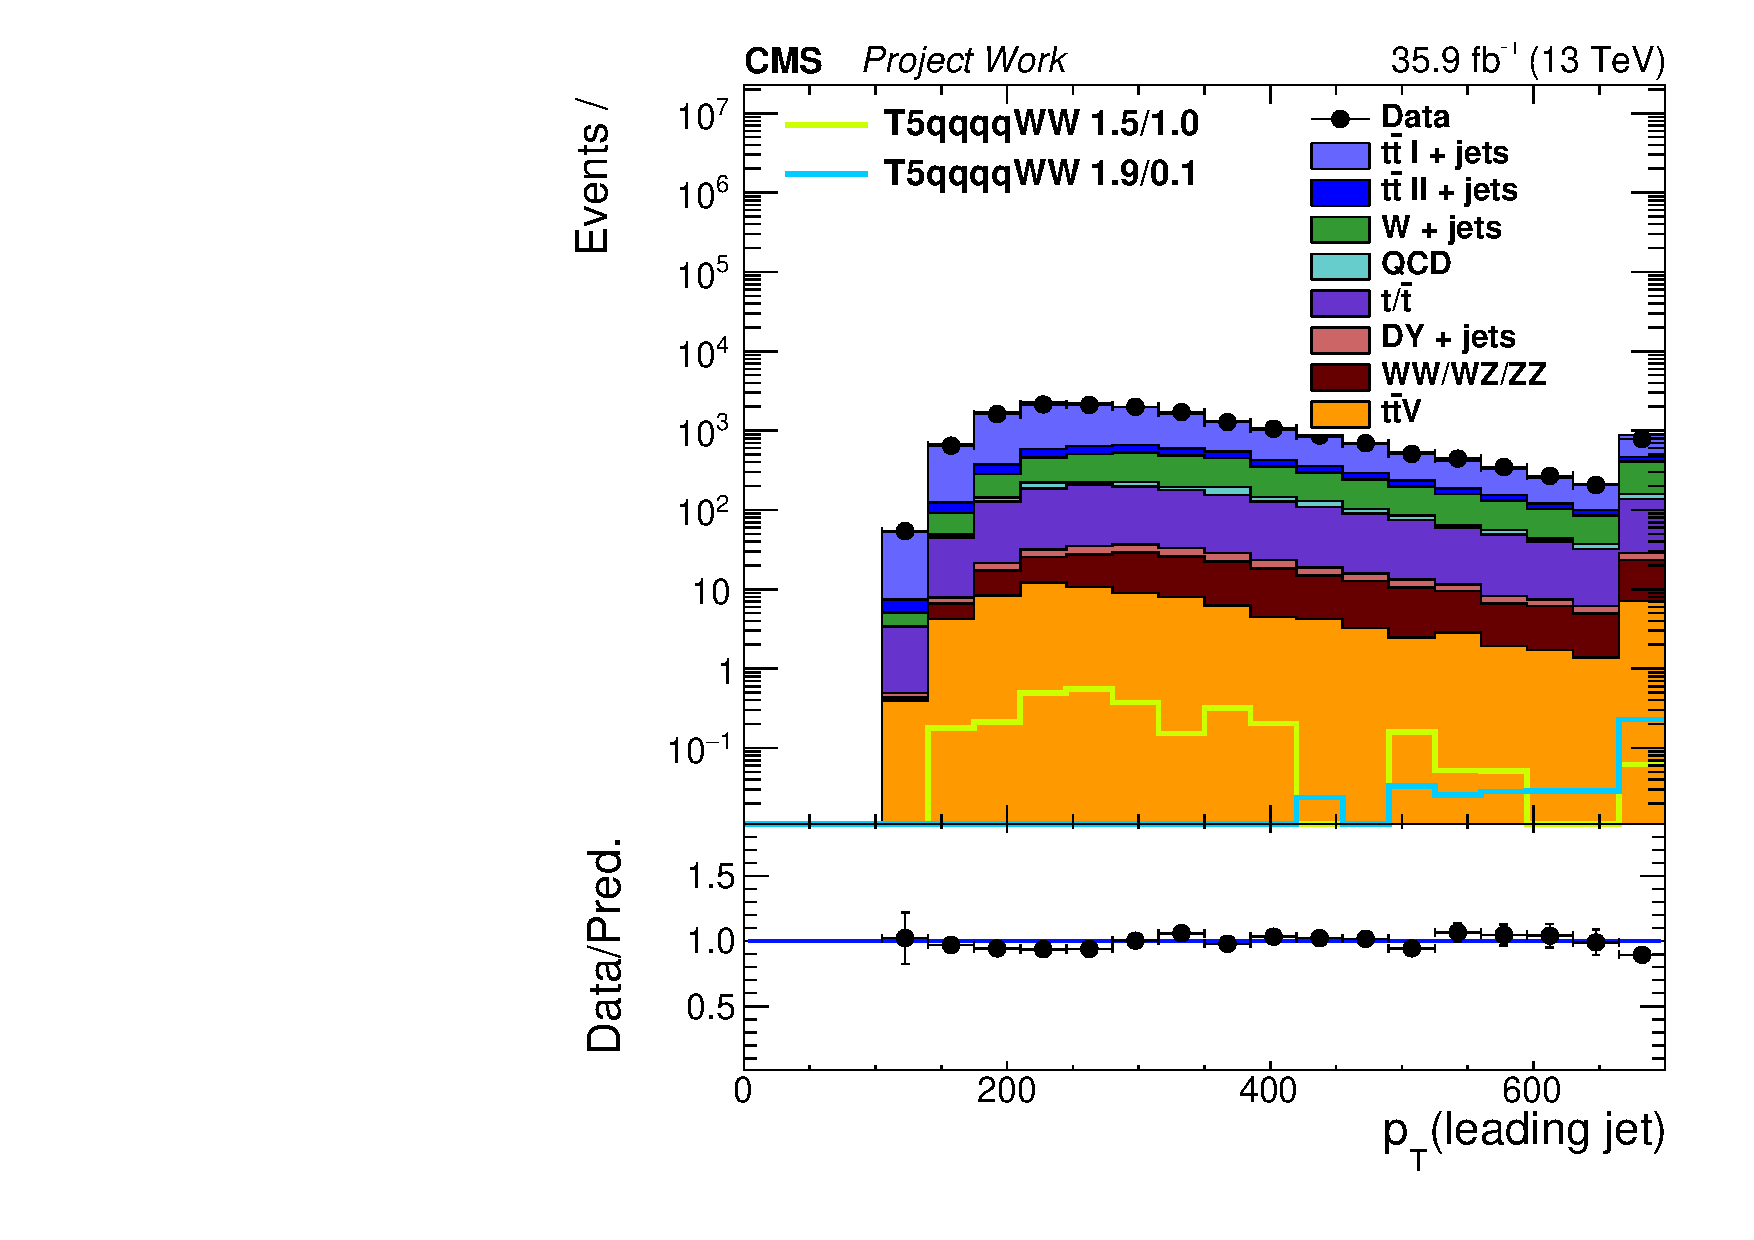
\includegraphics[angle=0,width=.32\textwidth]{Plots//analysis/control_Plots/mu/st250_ht500_njet4-5_nbtag1/leading_JetPtProject_Work.pdf}}
    \subfigure[$n_{\textrm{vertex}}$]{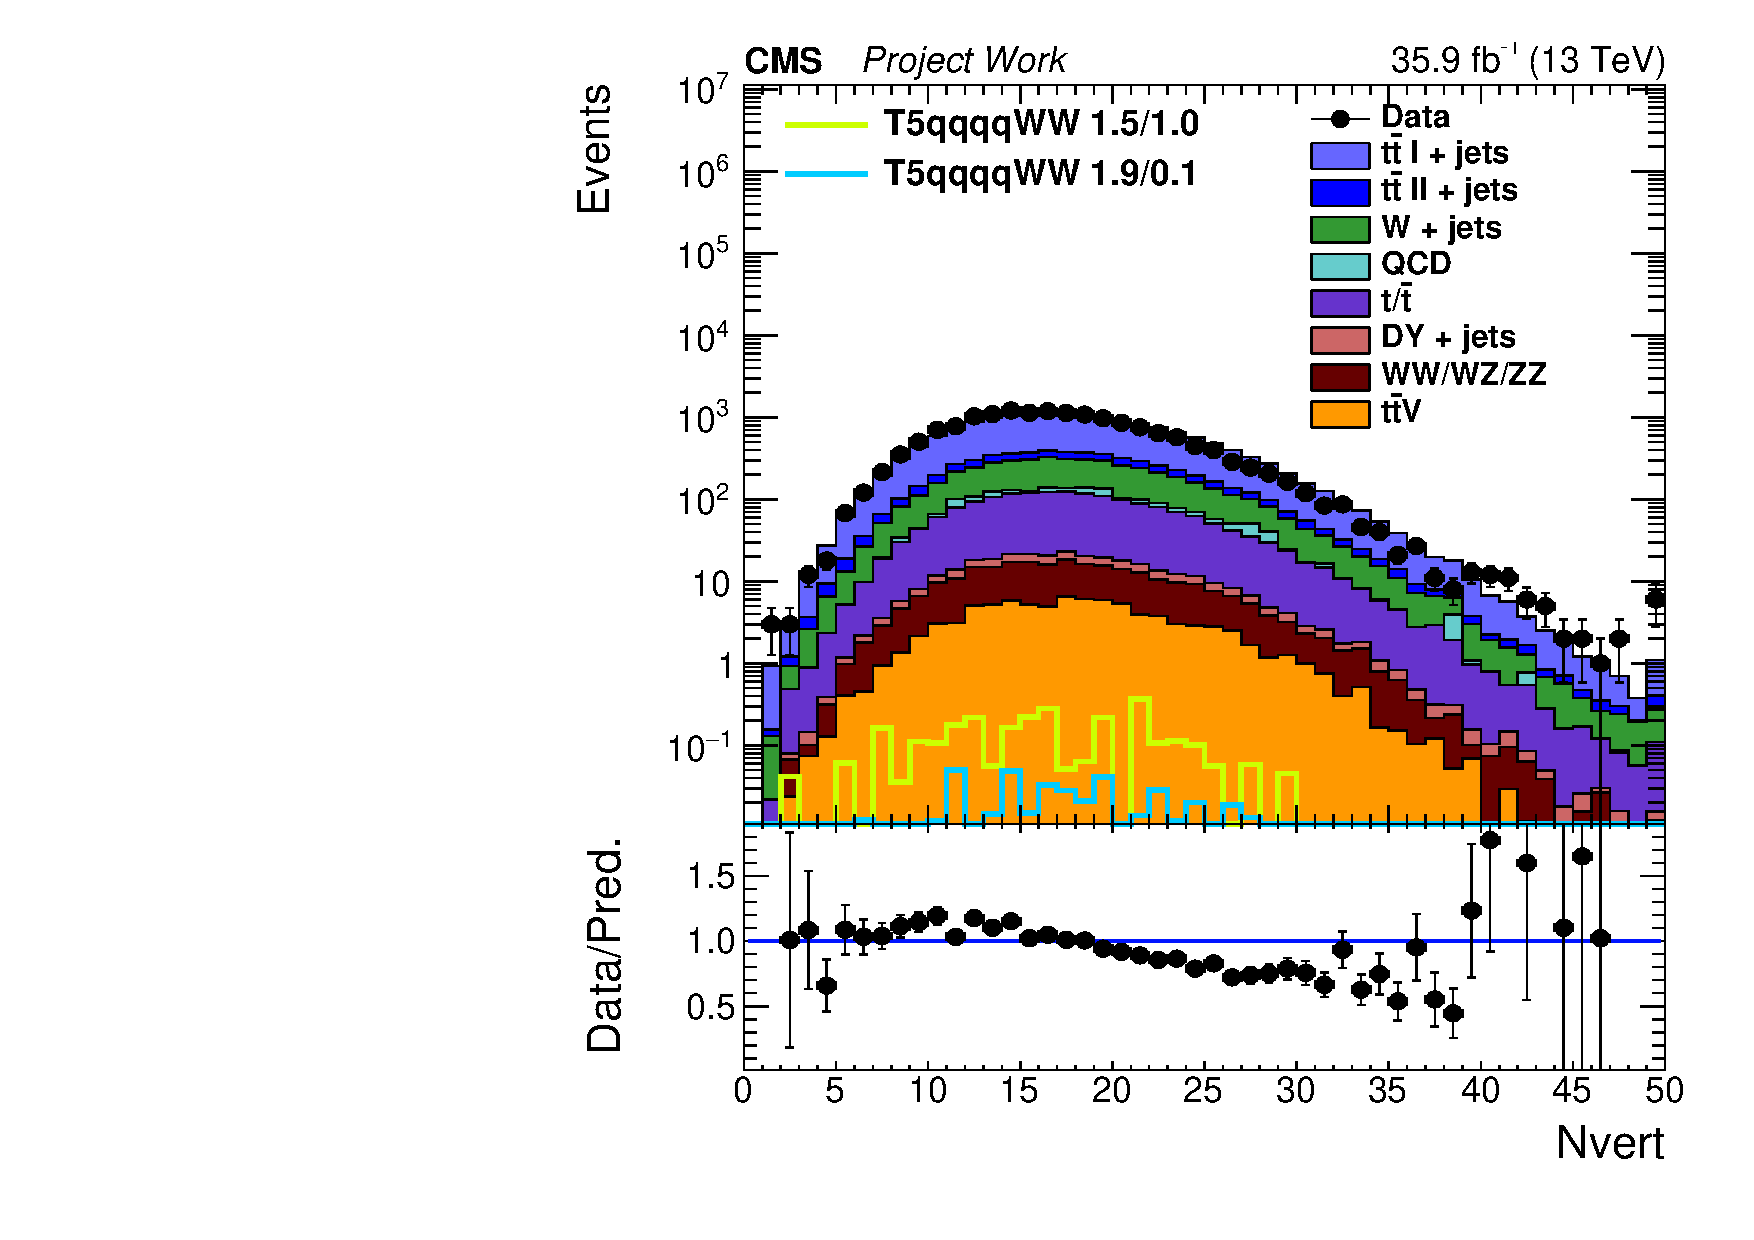
\includegraphics[angle=0,width=.32\textwidth]       {Plots//analysis/control_Plots/mu/st250_ht500_njet4-5_nbtag1/nVertProject_Work.pdf}}\\
    \subfigure[$p_T(l)$]{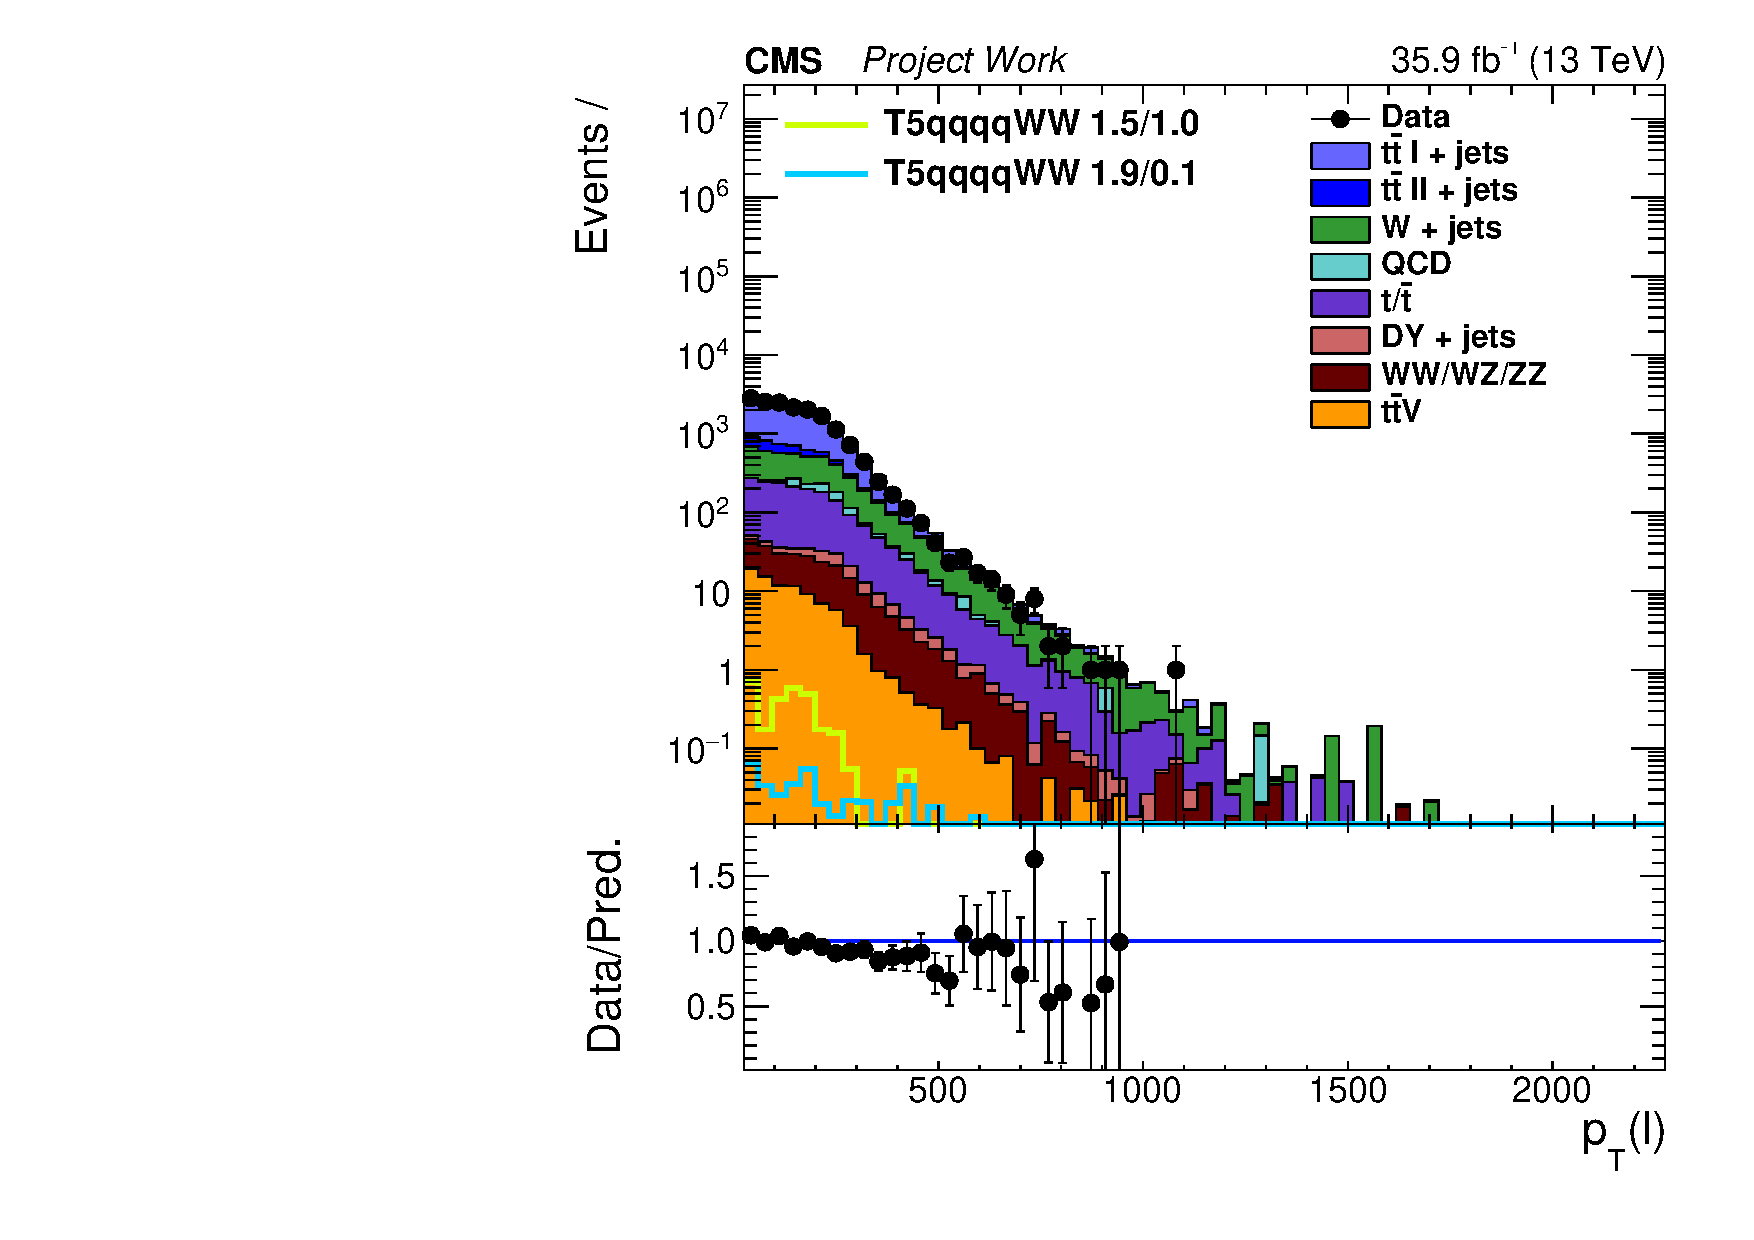
\includegraphics[angle=0,width=.32\textwidth]               {Plots//analysis/control_Plots/mu/st250_ht500_njet4-5_nbtag1/leptonPtProject_Work.pdf}}
    \subfigure[$m_{T2}$]{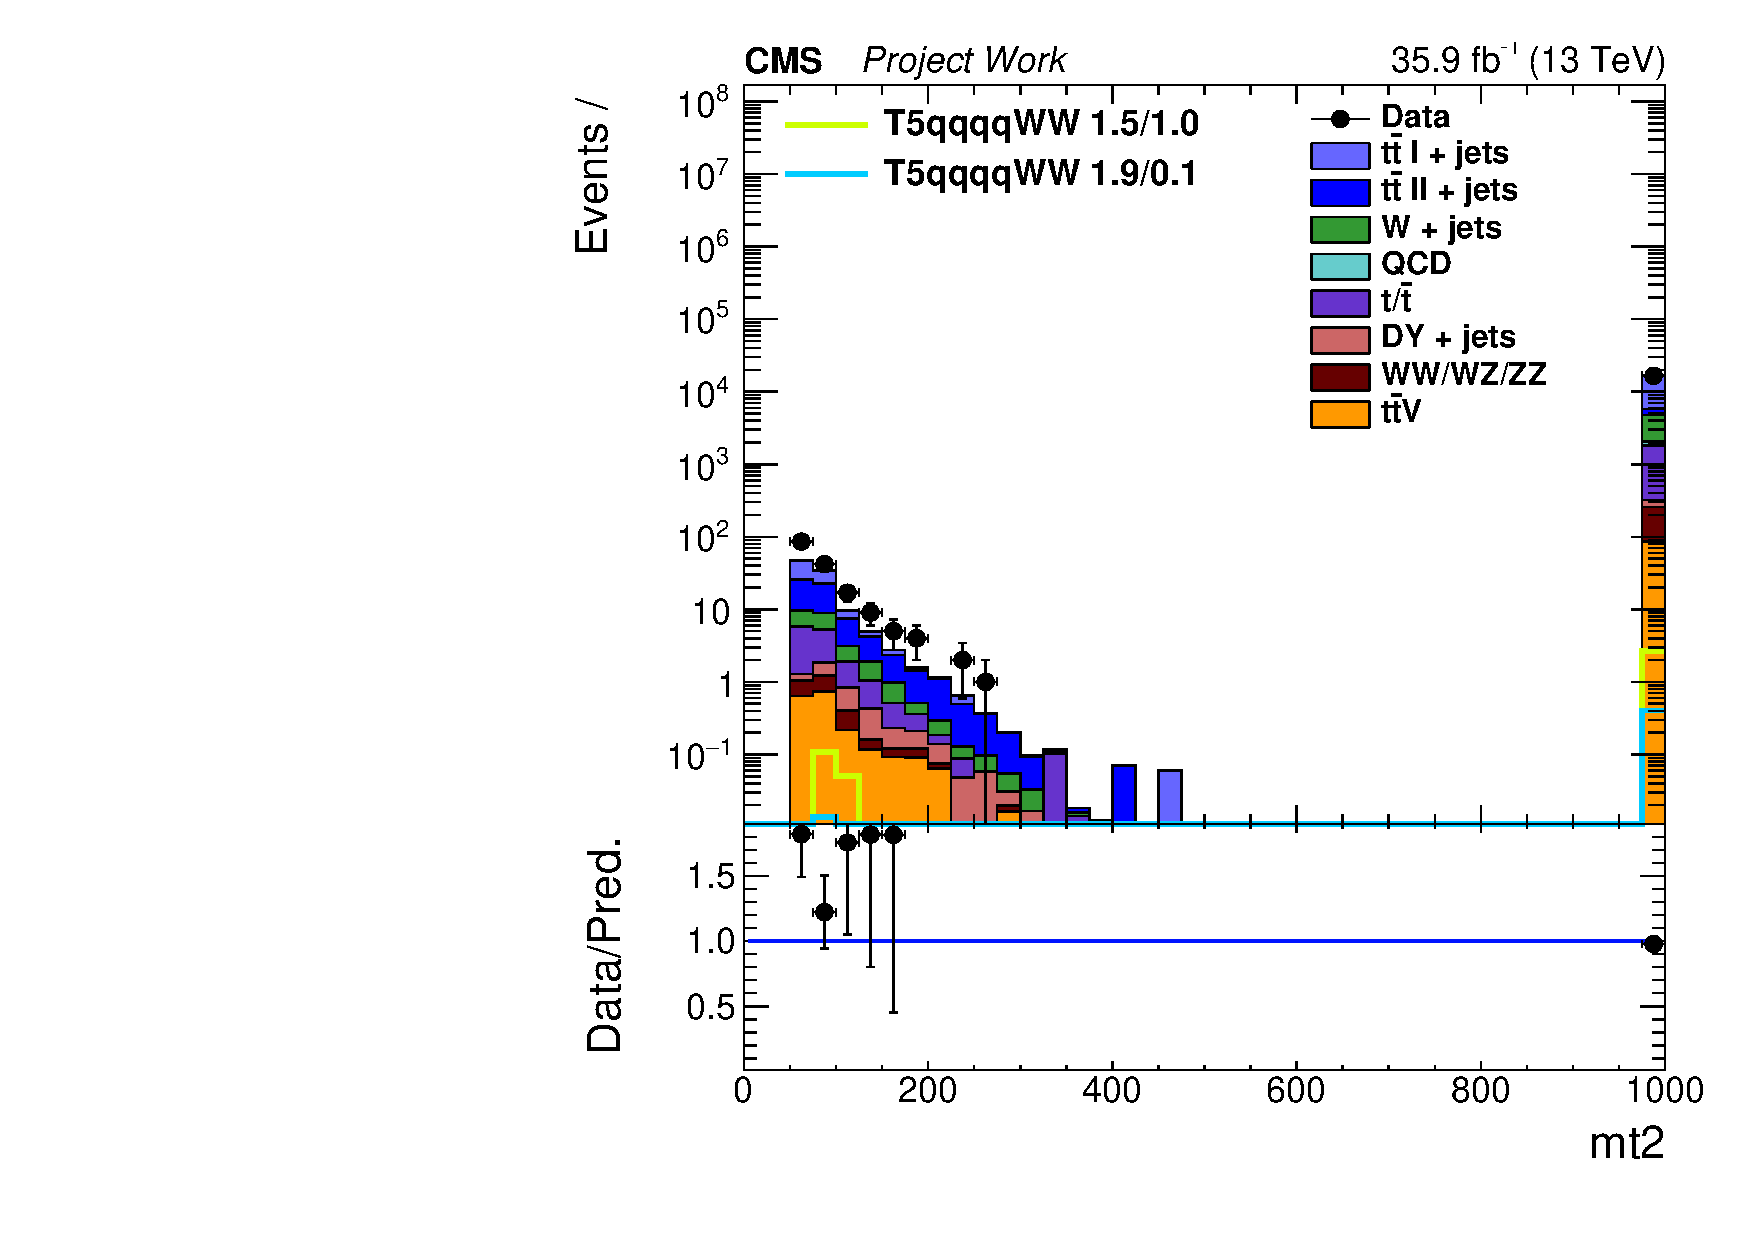
\includegraphics[angle=0,width=.32\textwidth]              {Plots//analysis/control_Plots/mu/st250_ht500_njet4-5_nbtag1/iso_MT2Project_Work.pdf}}
    \subfigure[miniIsolation$(l)$]{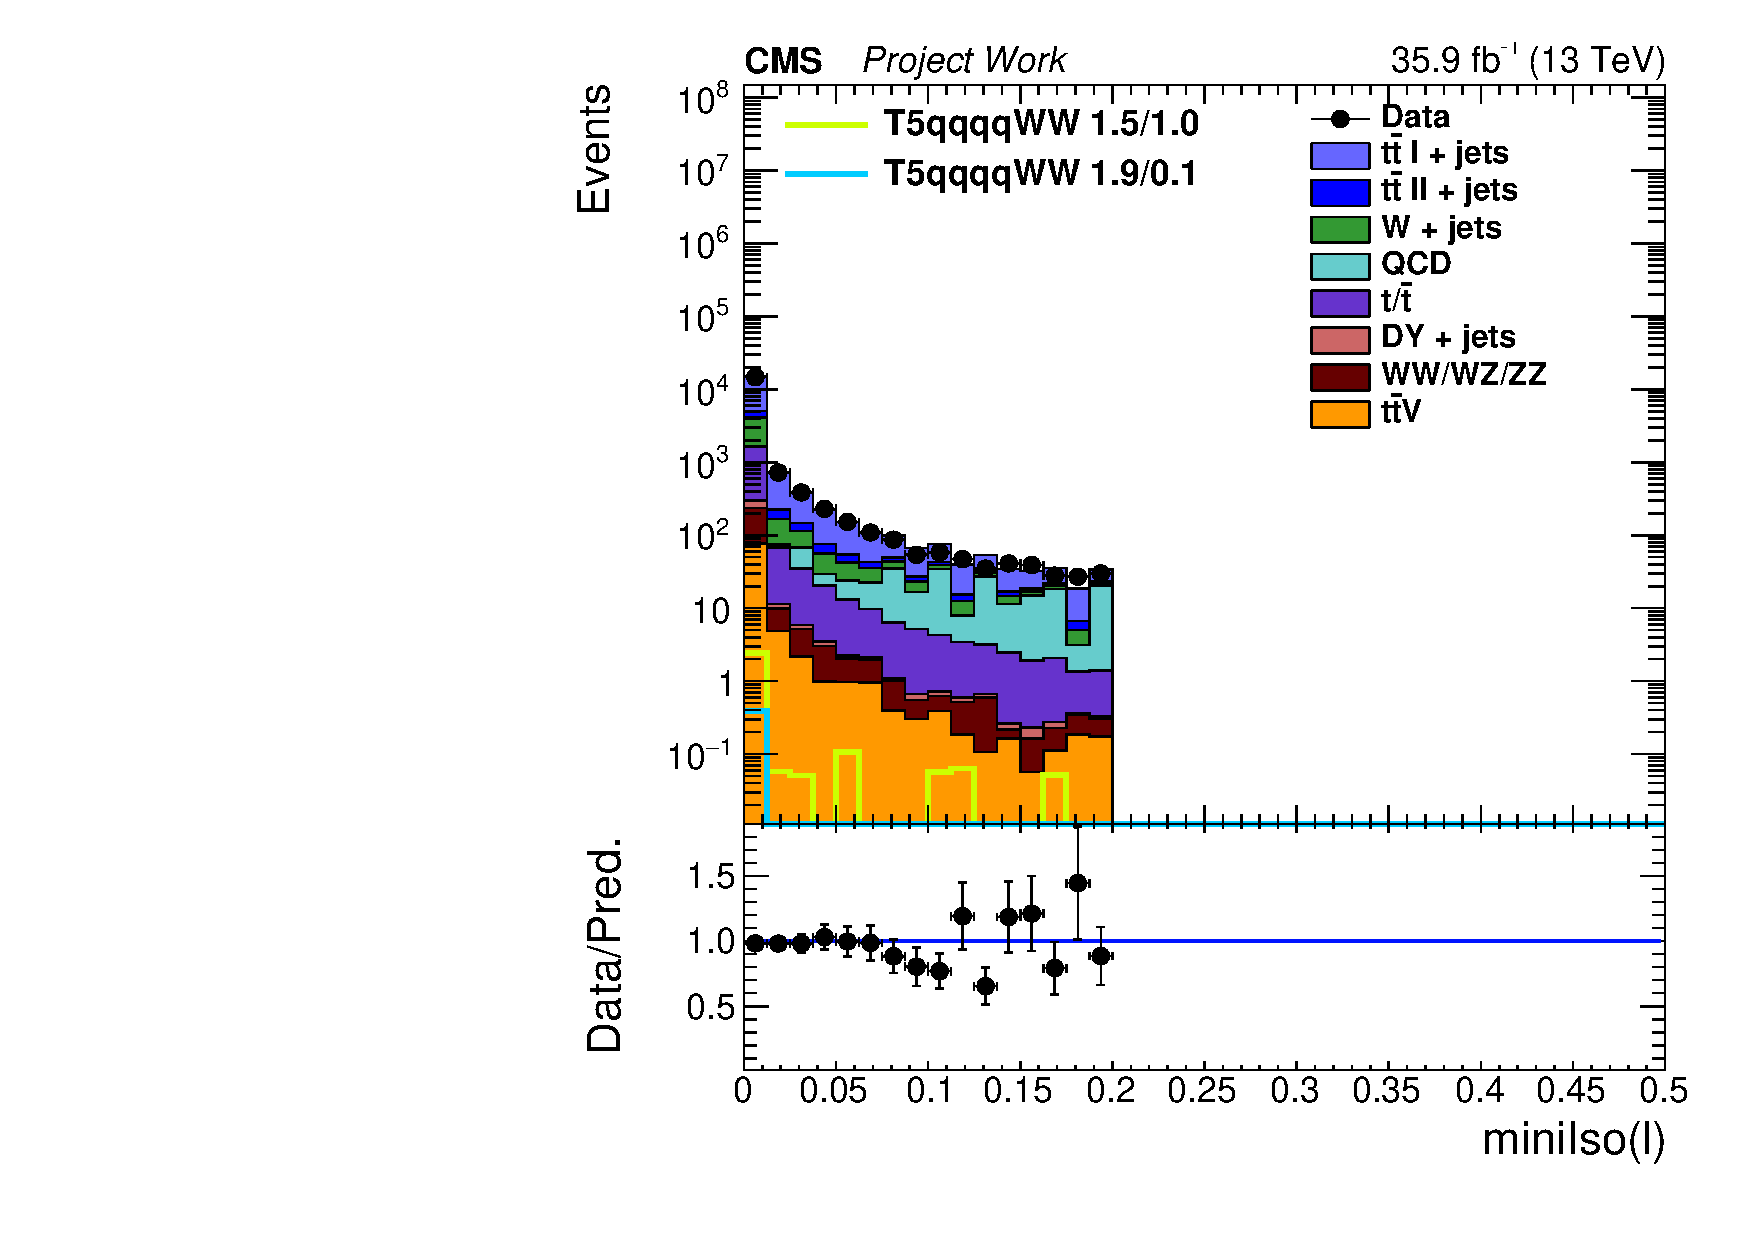
\includegraphics[angle=0,width=.32\textwidth]     {Plots//analysis/control_Plots/mu/st250_ht500_njet4-5_nbtag1/leptonminiIsoProject_Work.pdf}}\\
    \subfigure[\HT]{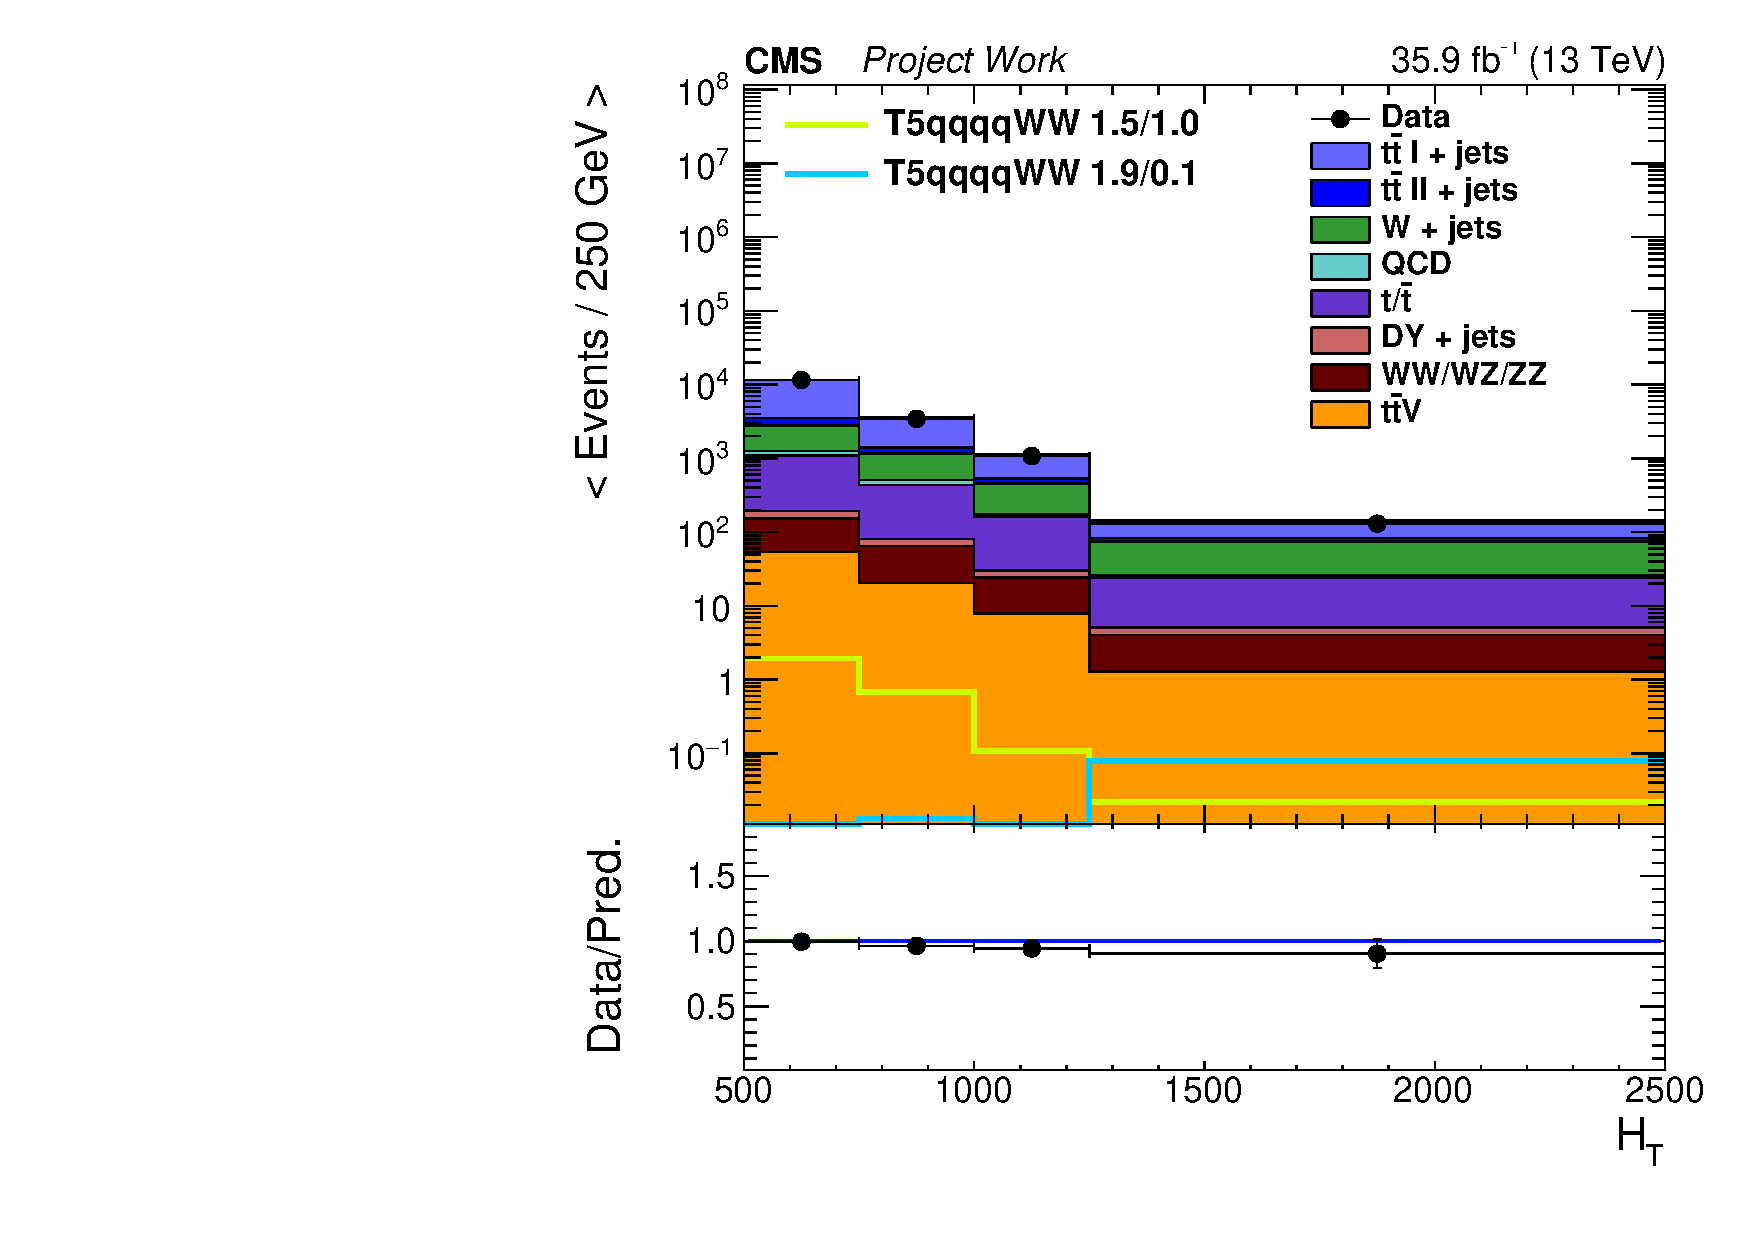
\includegraphics[angle=0,width=.32\textwidth]                    {Plots//analysis/control_Plots/mu/st250_ht500_njet4-5_nbtag1/htJet30jProject_Work.pdf}}
    \subfigure[\LT]{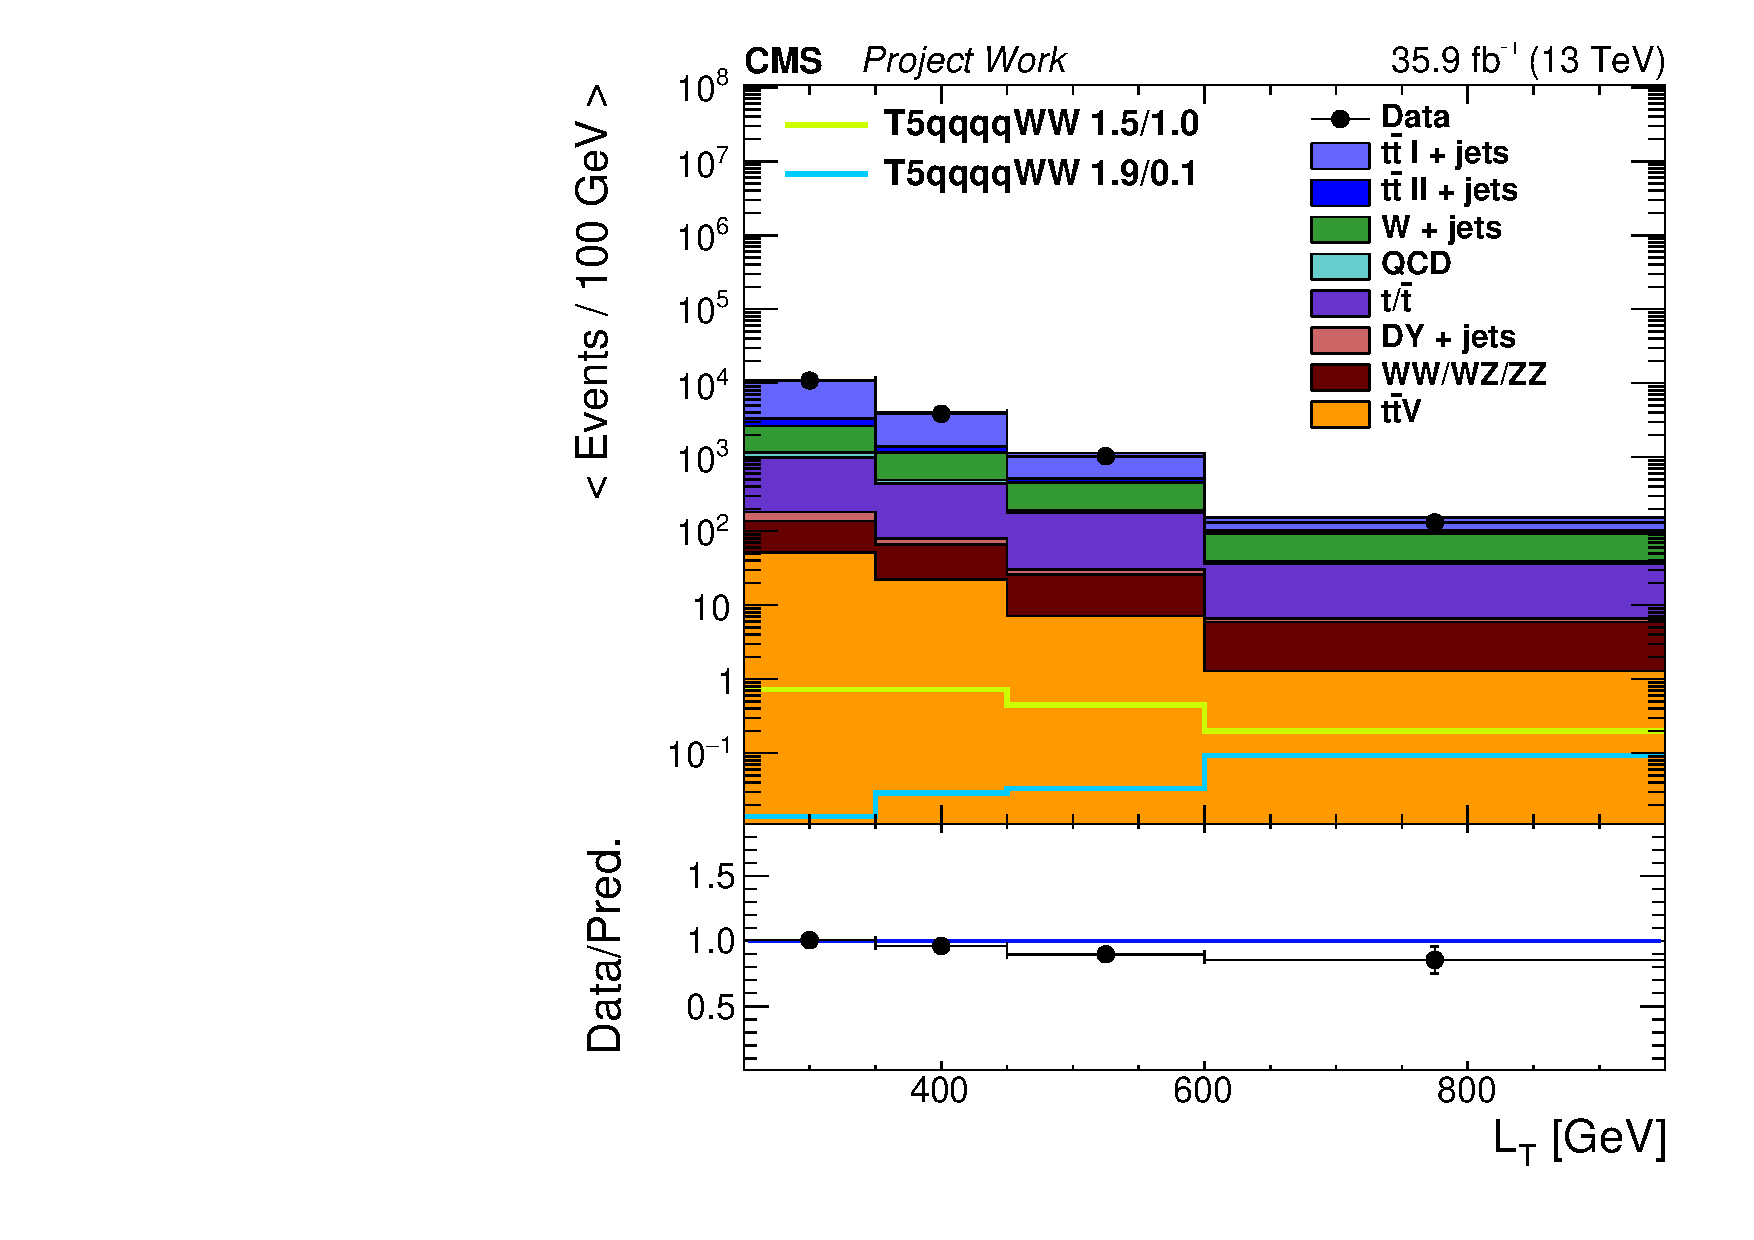
\includegraphics[angle=0,width=.32\textwidth]                    {Plots//analysis/control_Plots/mu/st250_ht500_njet4-5_nbtag1/LTProject_Work.pdf}}
    \subfigure[\DF]{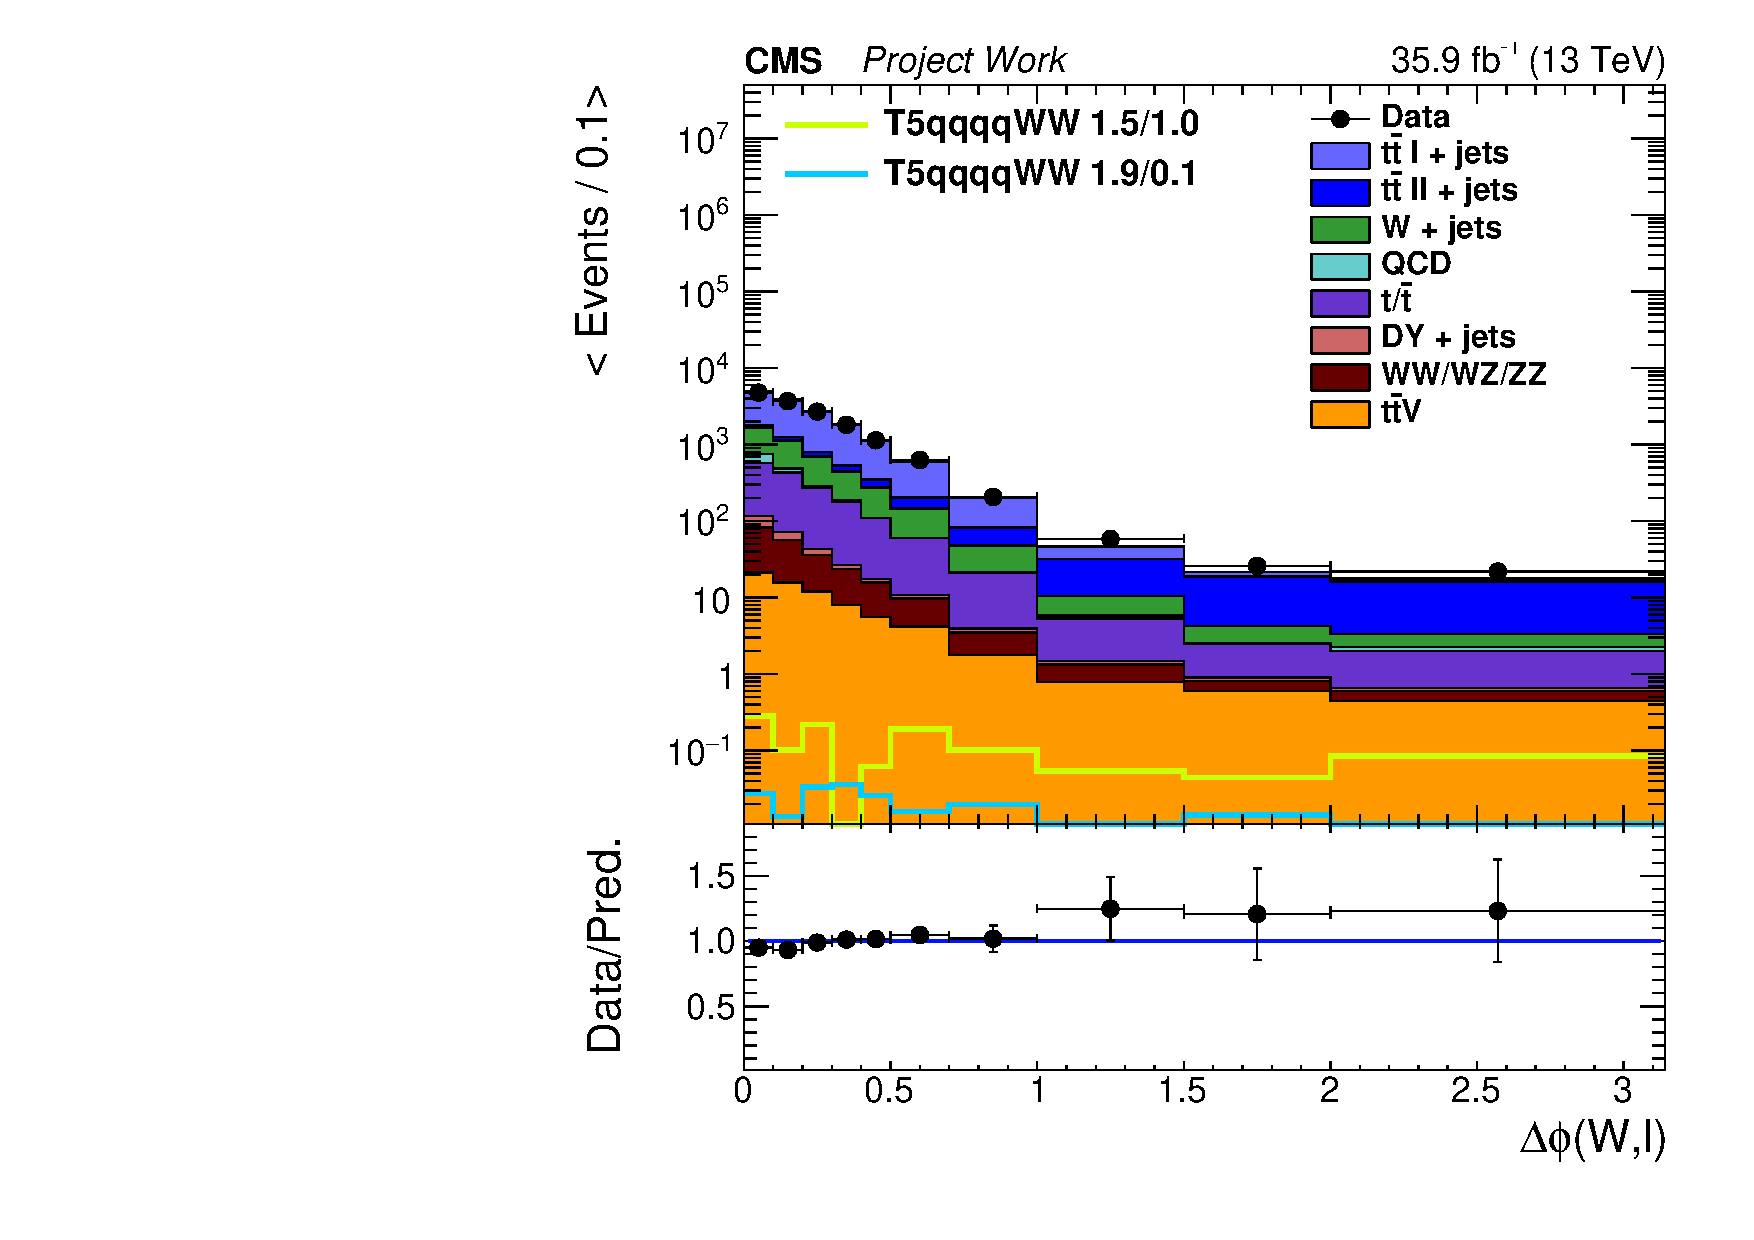
\includegraphics[angle=0,width=.32\textwidth]                    {Plots//analysis/control_Plots/mu/st250_ht500_njet4-5_nbtag1/deltaPhi_Wl_wideProject_Work.pdf}}

    \caption{Distribution of kinematic observables after requiring $\HT >$~500~\GeV, $\LT >$~250~\GeV, $4\leq$ jets $\leq5$  and  b-tagged jets (1 $\mu$ channel).
      %In order to blind the signal region, data events with large \DF (corresponding to the dynamic \DF cut) are excluded from the \DF plot.
    }
    \label{fig:0bmu_1B_4_5jets_CR}
  \end{center}
\end{figure}

\begin{figure}[p]
  \begin{center}
    \subfigure[\njet]{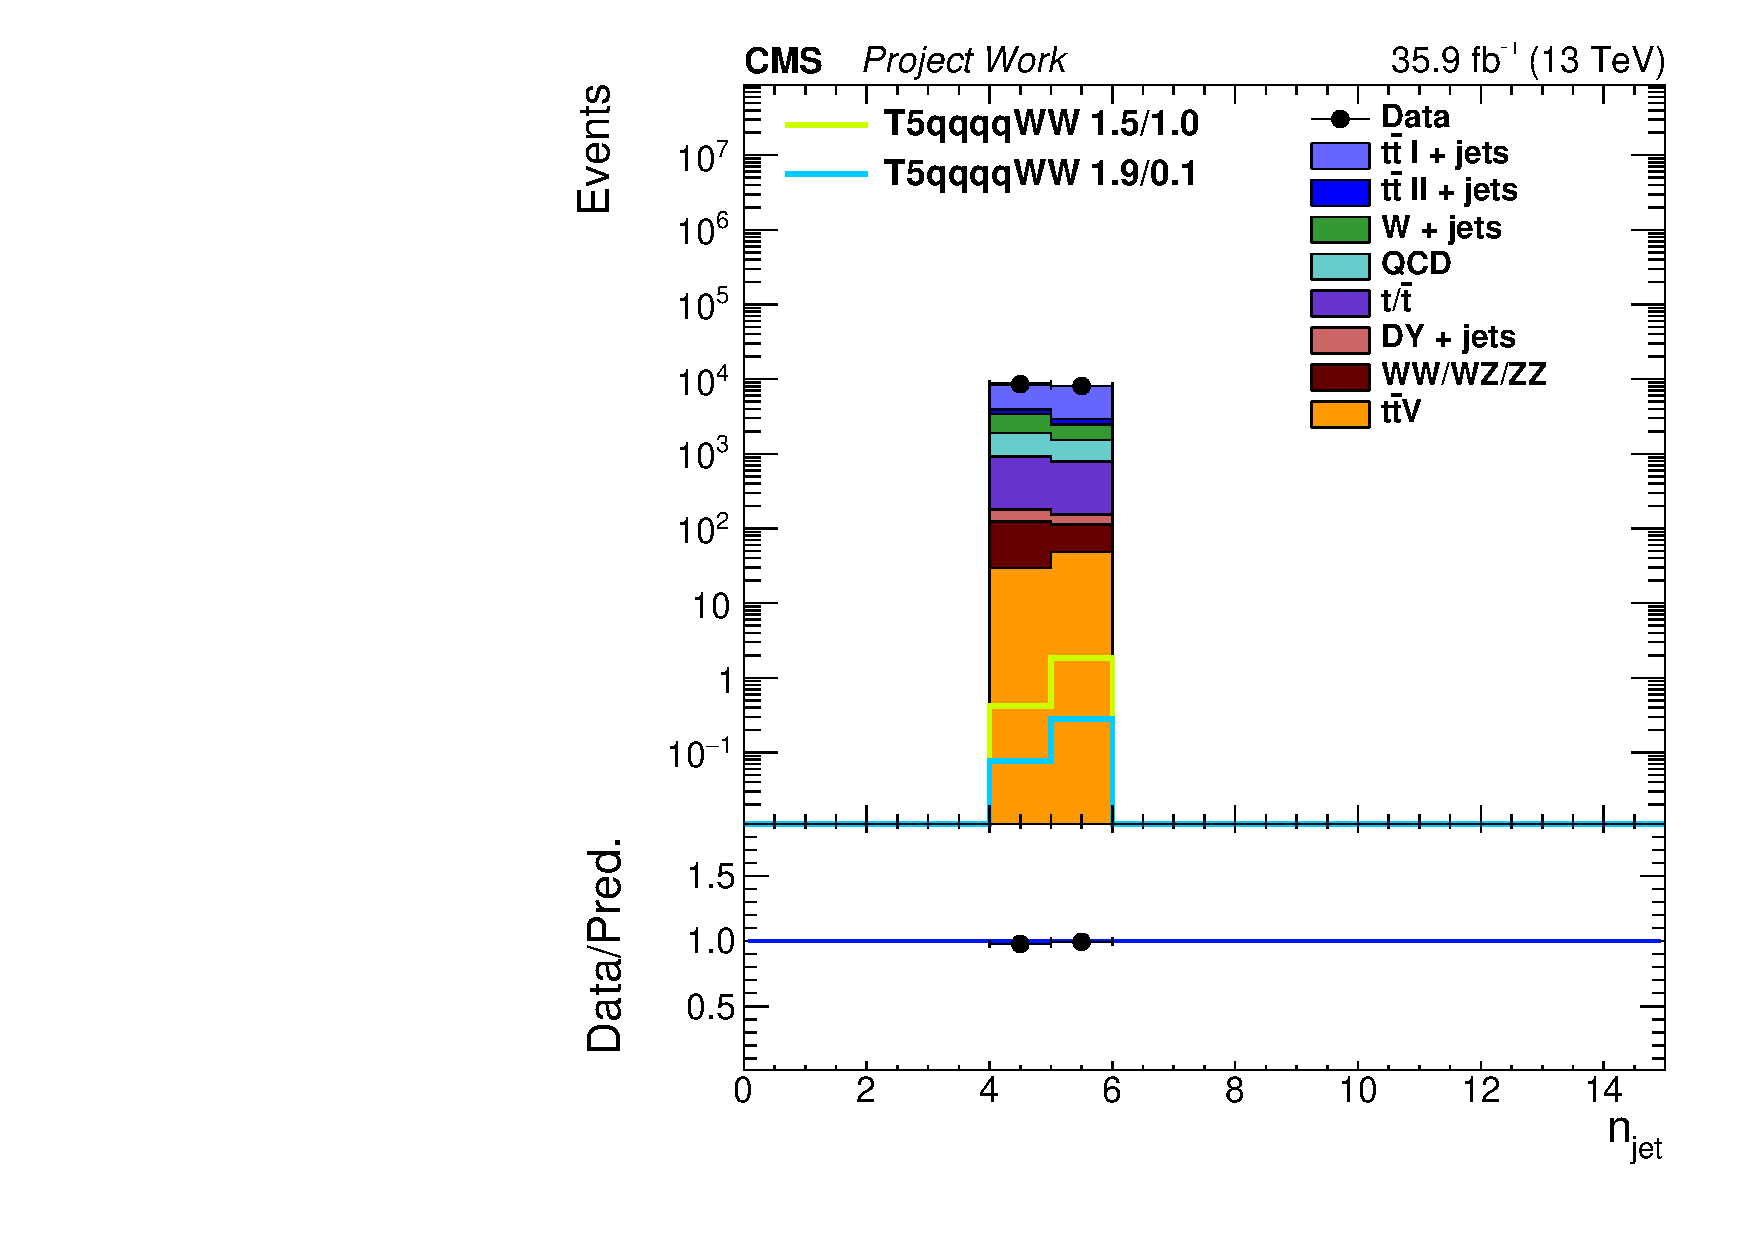
\includegraphics[angle=0,width=.32\textwidth]                  {Plots//analysis/control_Plots/ele/st250_ht500_njet4-5_nbtag1/nJet30Project_Work.pdf}}
    \subfigure[$p_T(\textrm{1st jet})$]{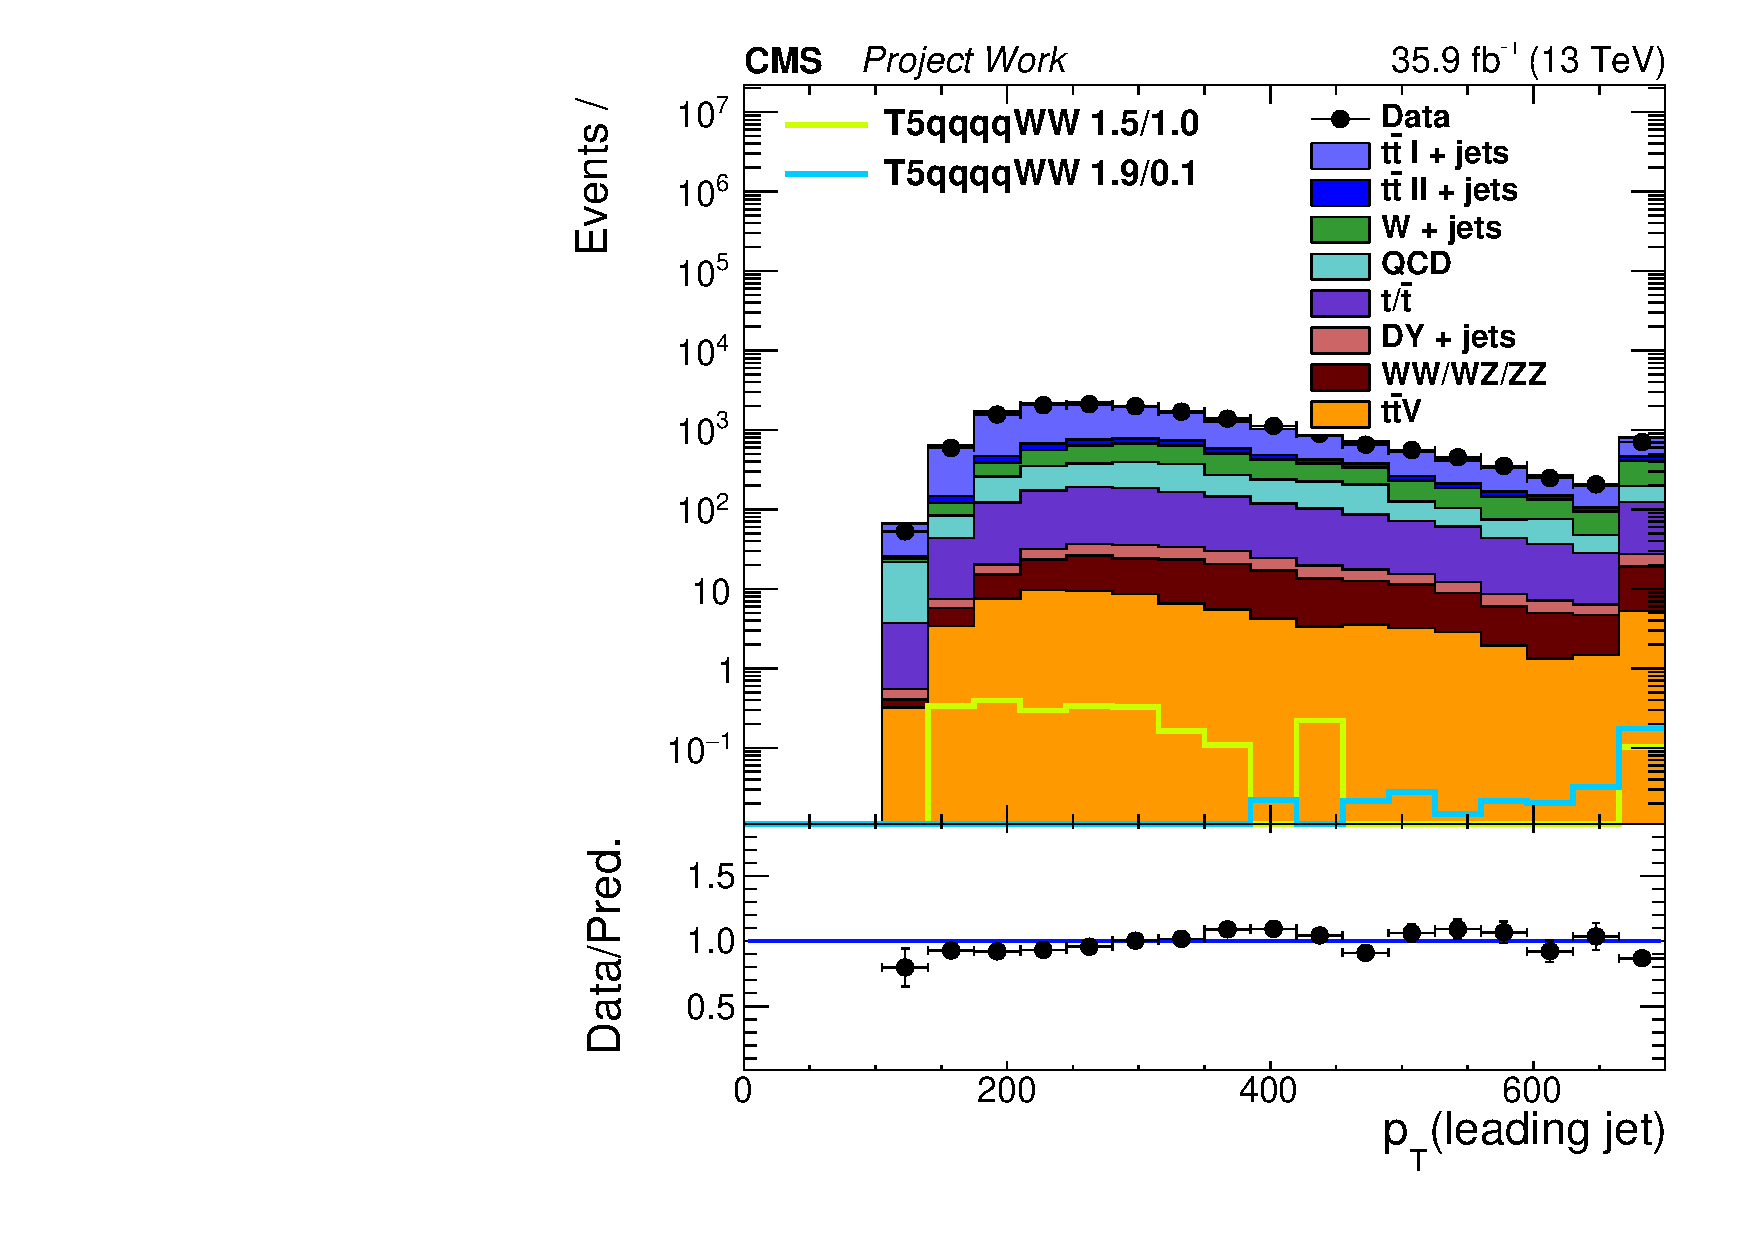
\includegraphics[angle=0,width=.32\textwidth]{Plots//analysis/control_Plots/ele/st250_ht500_njet4-5_nbtag1/leading_JetPtProject_Work.pdf}}
    \subfigure[$n_{\textrm{vertex}}$]{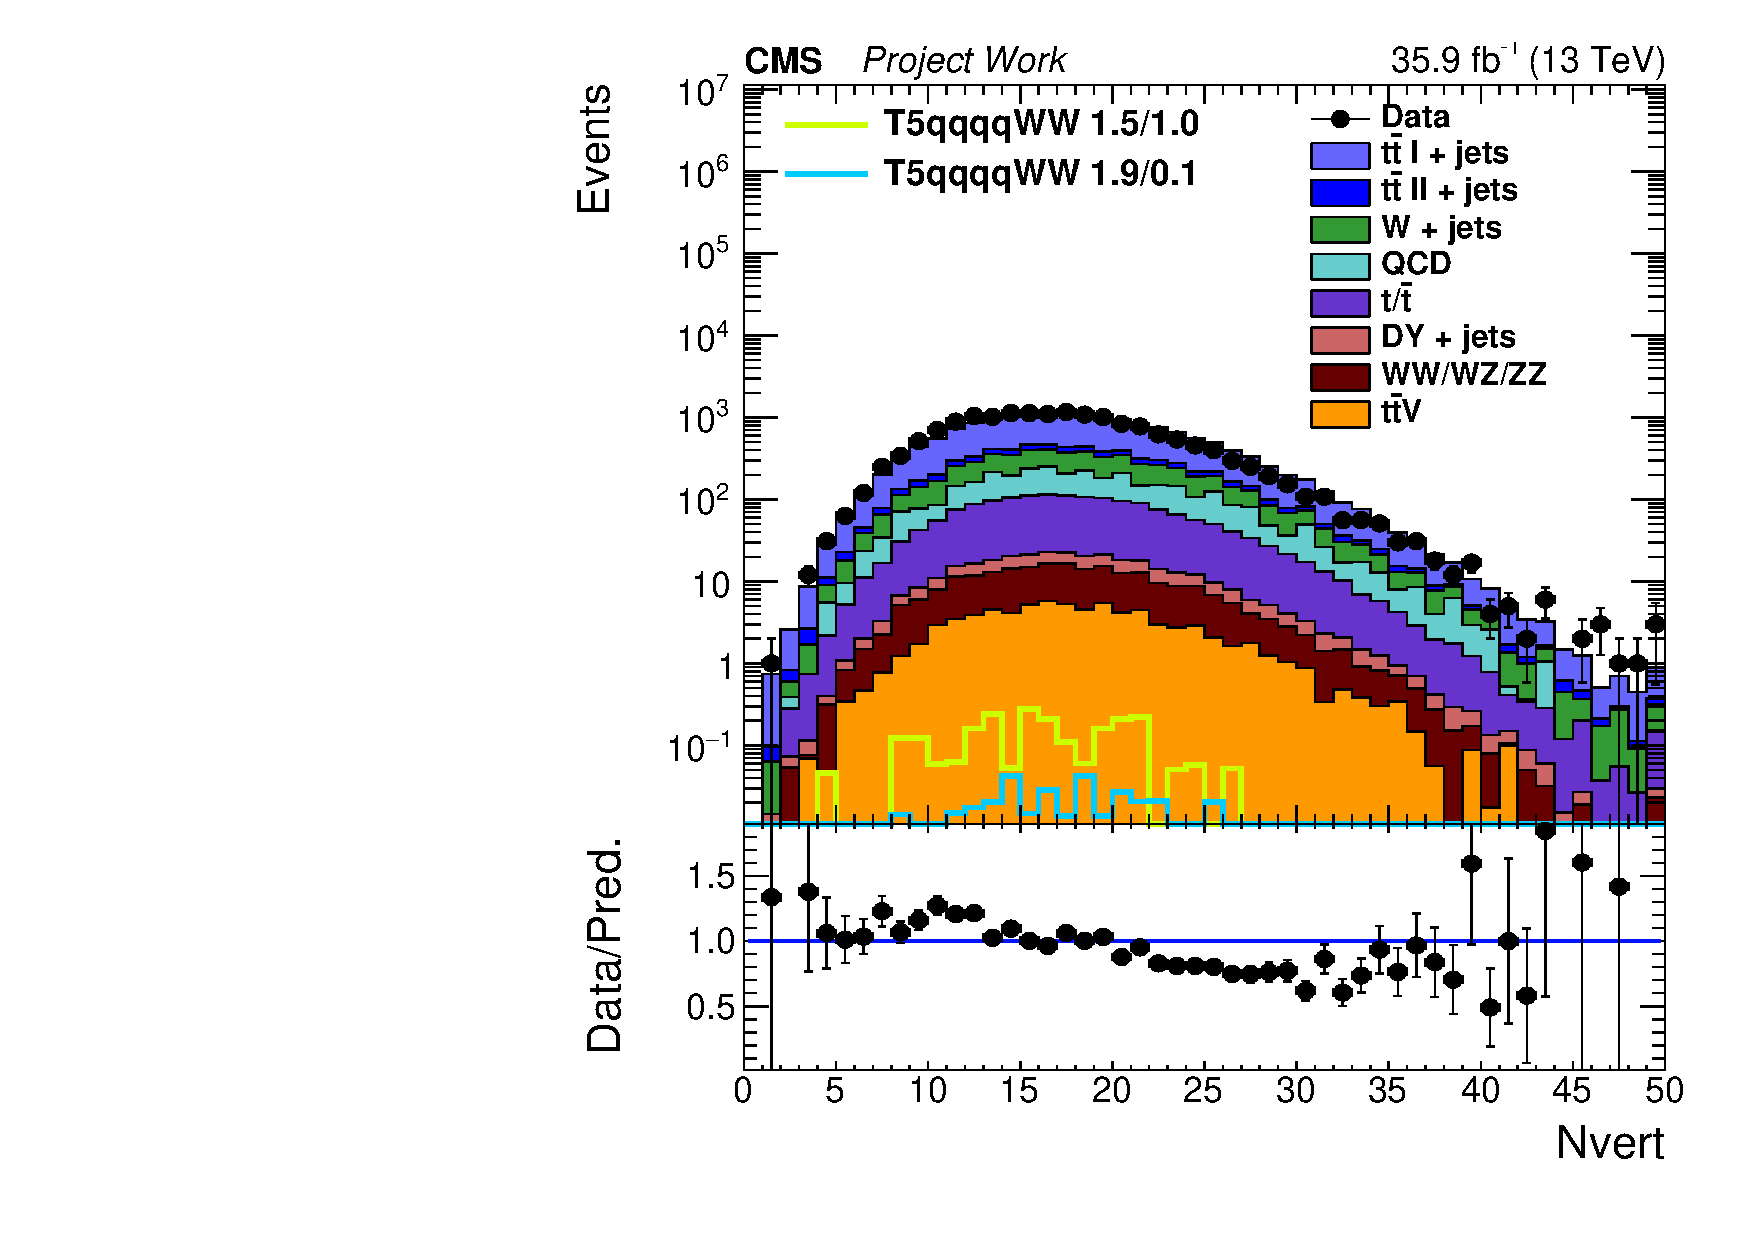
\includegraphics[angle=0,width=.32\textwidth]       {Plots//analysis/control_Plots/ele/st250_ht500_njet4-5_nbtag1/nVertProject_Work.pdf}}\\
    \subfigure[$p_T(l)$]{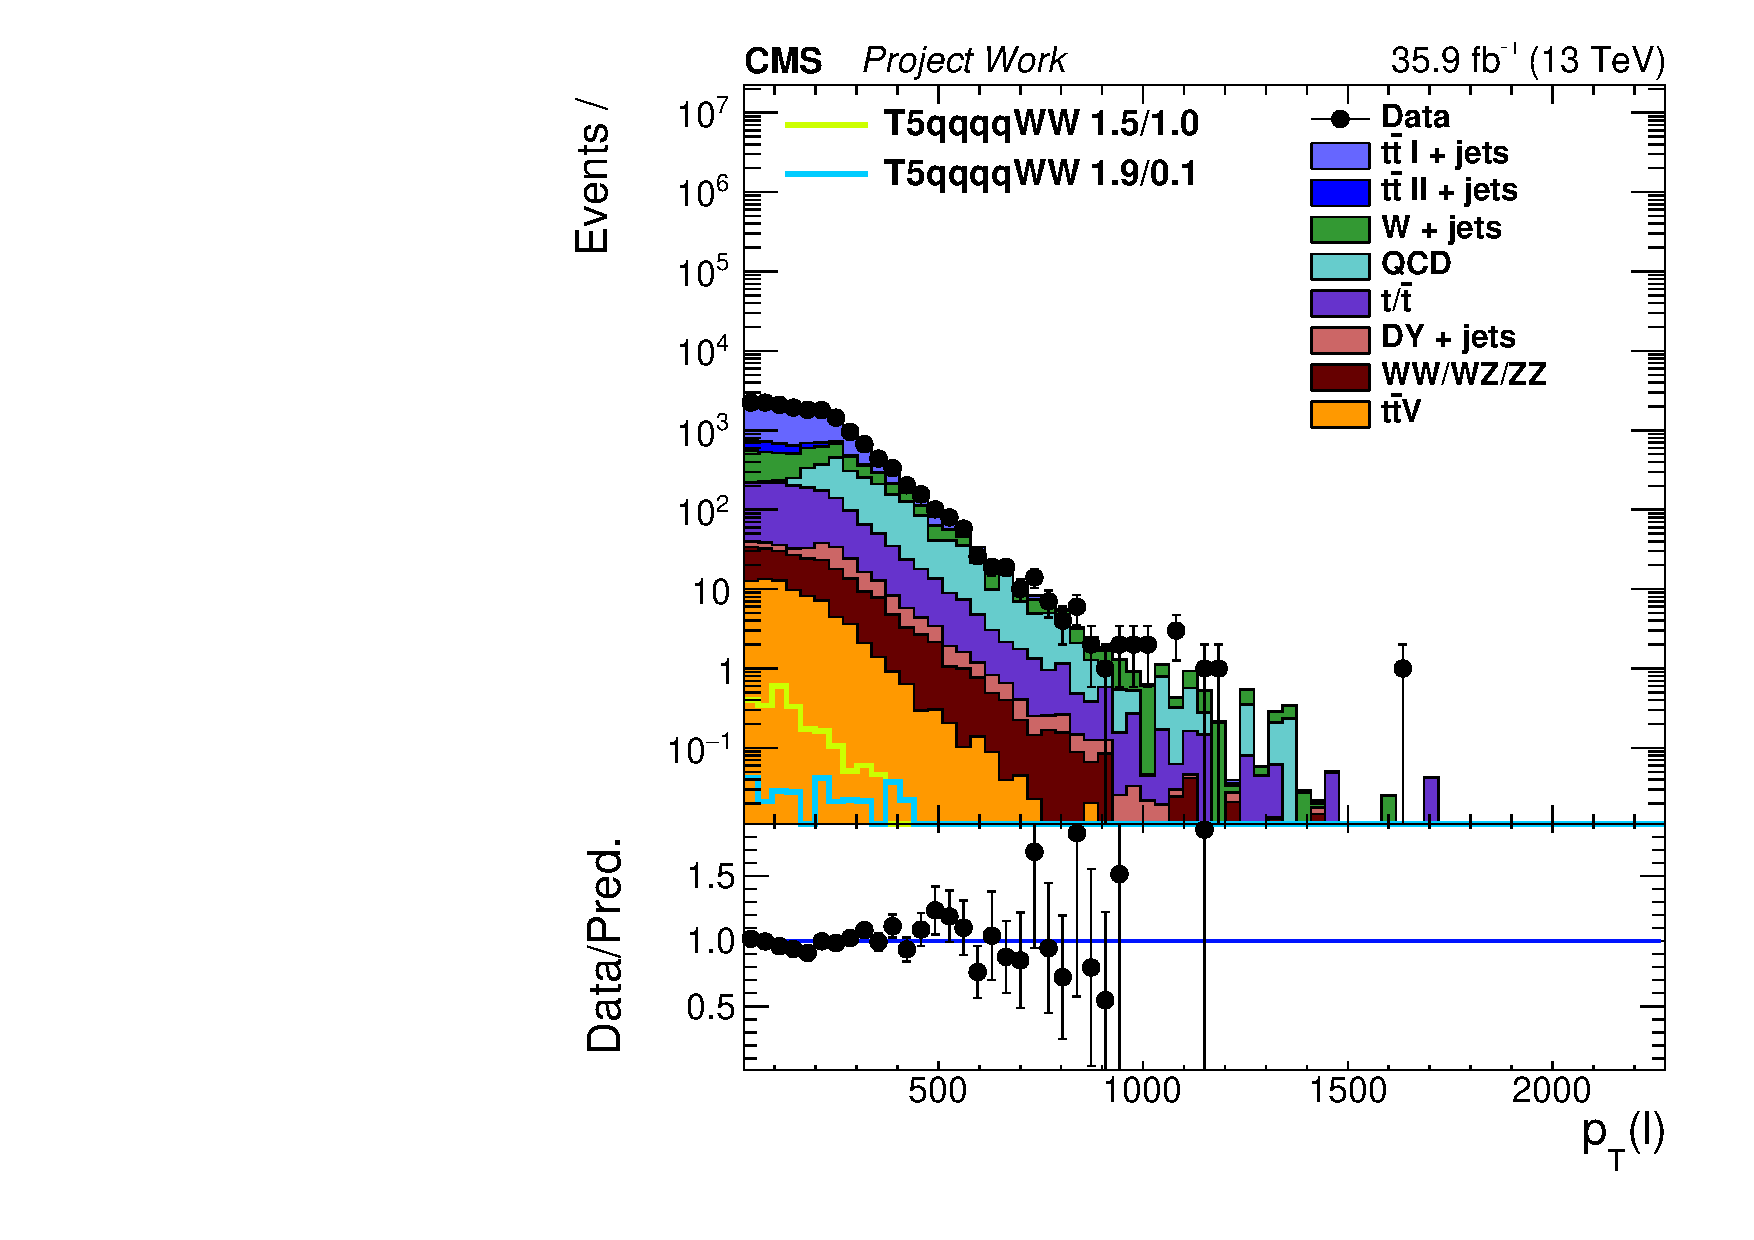
\includegraphics[angle=0,width=.32\textwidth]               {Plots//analysis/control_Plots/ele/st250_ht500_njet4-5_nbtag1/leptonPtProject_Work.pdf}}
    \subfigure[$m_{T2}$]{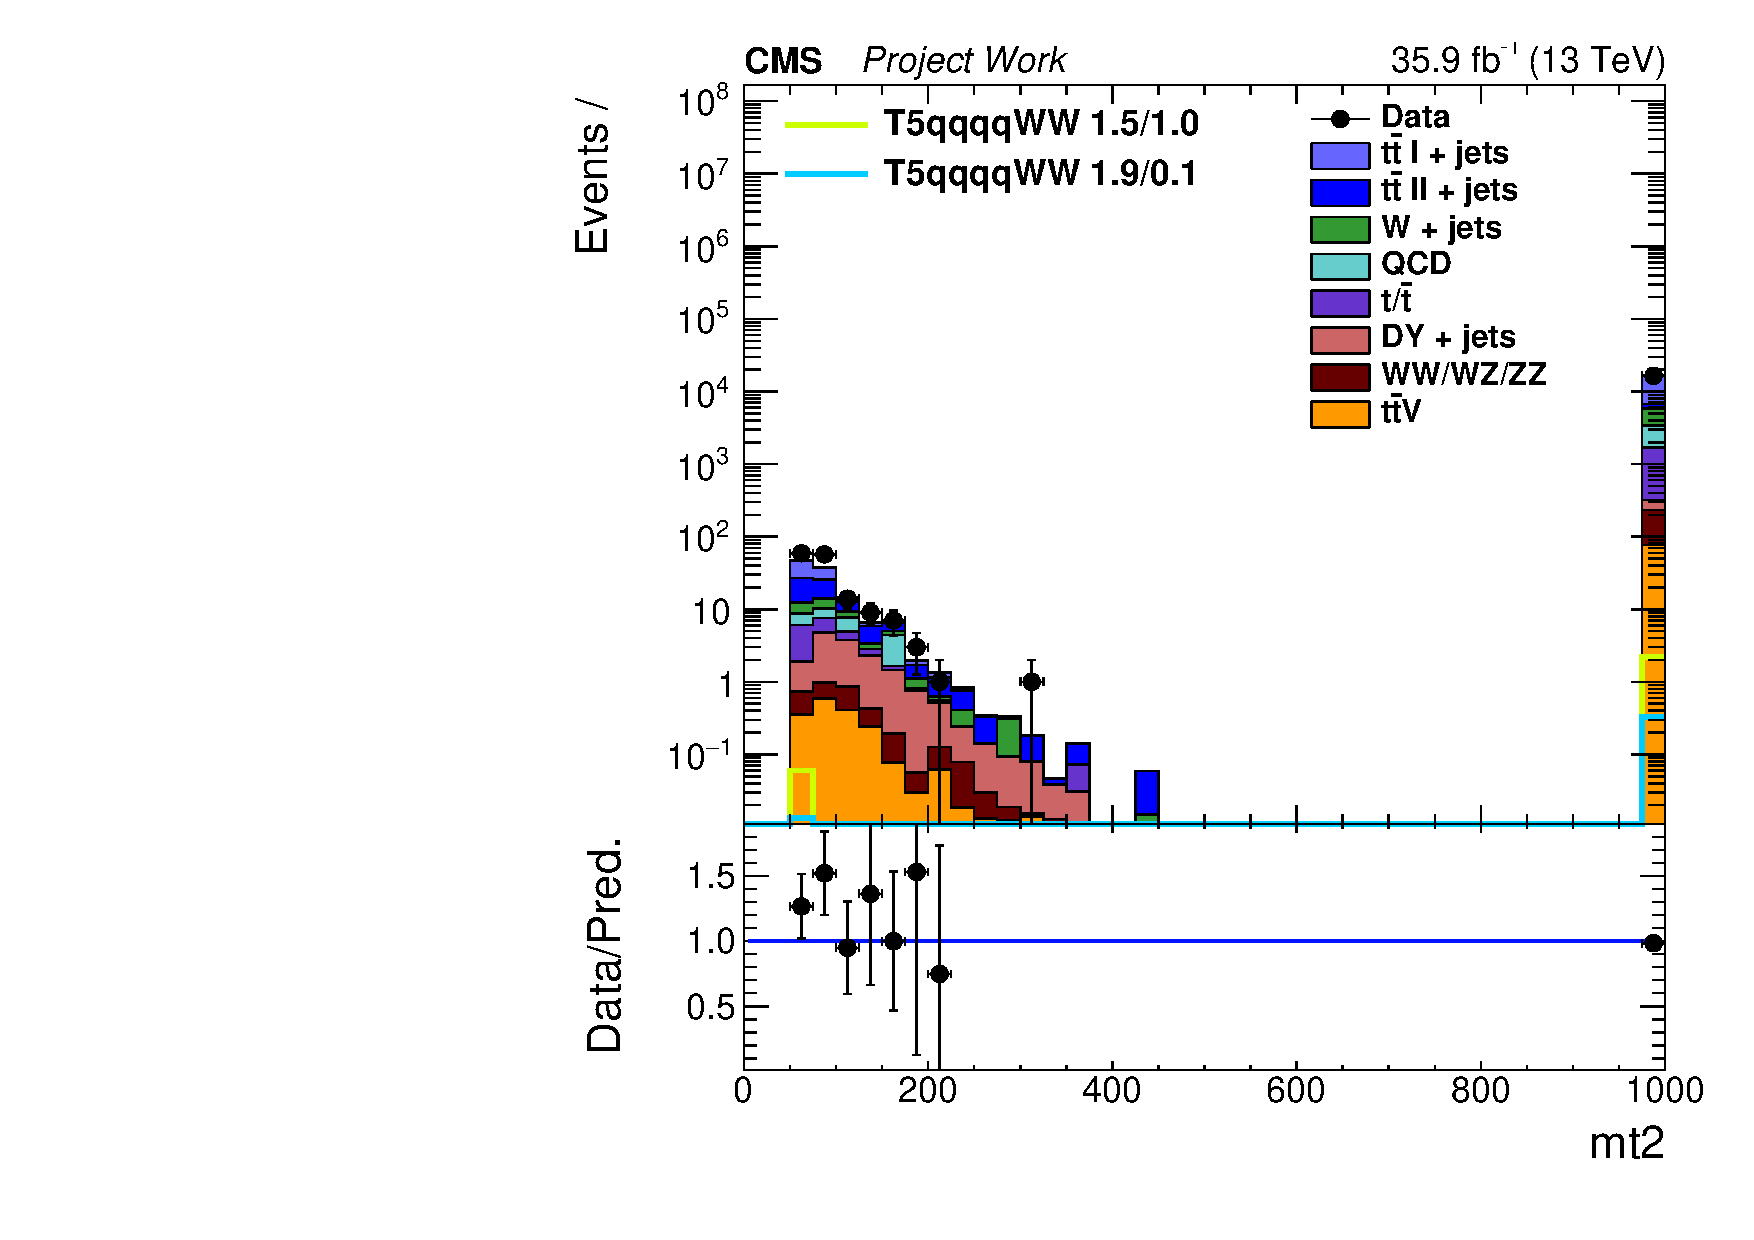
\includegraphics[angle=0,width=.32\textwidth]              {Plots//analysis/control_Plots/ele/st250_ht500_njet4-5_nbtag1/iso_MT2Project_Work.pdf}}
    \subfigure[miniIsolation$(l)$]{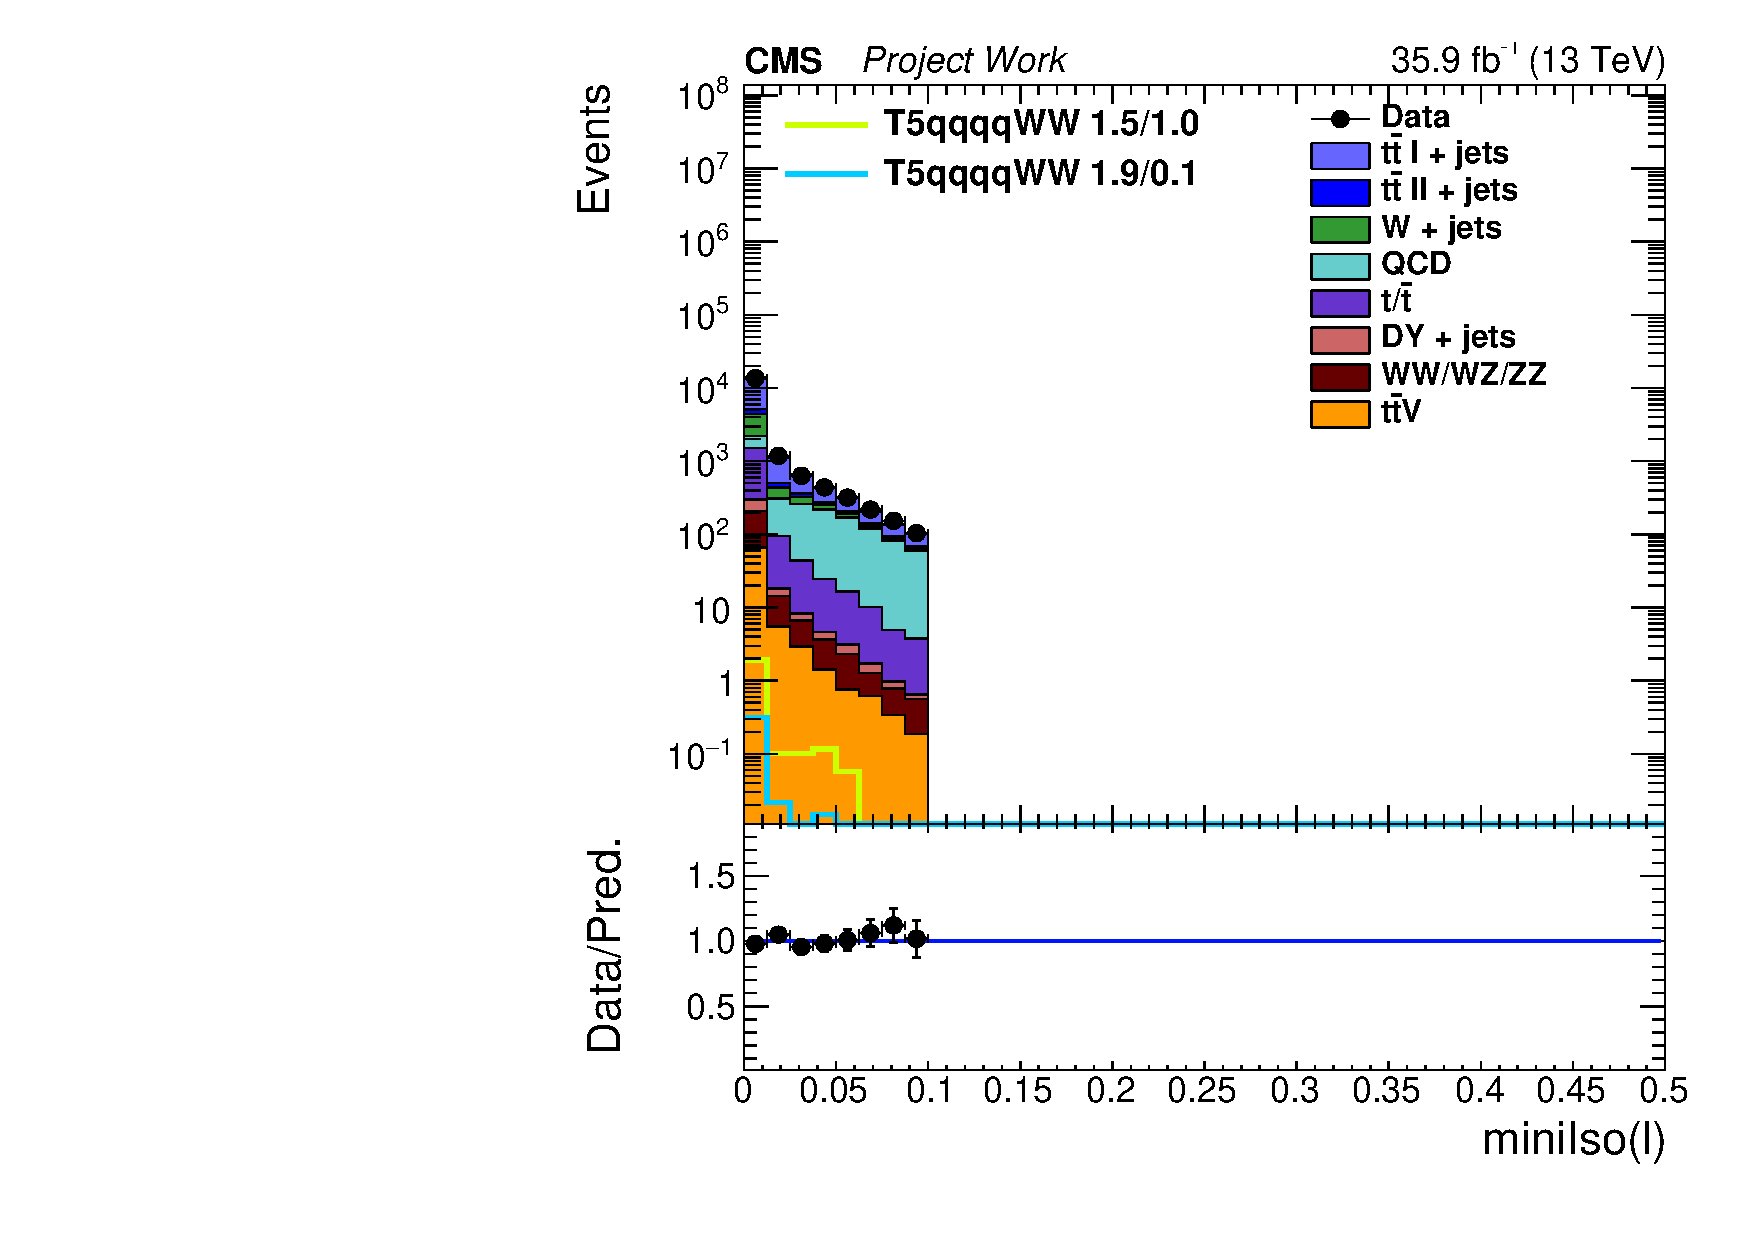
\includegraphics[angle=0,width=.32\textwidth]     {Plots//analysis/control_Plots/ele/st250_ht500_njet4-5_nbtag1/leptonminiIsoProject_Work.pdf}}\\
    \subfigure[\HT]{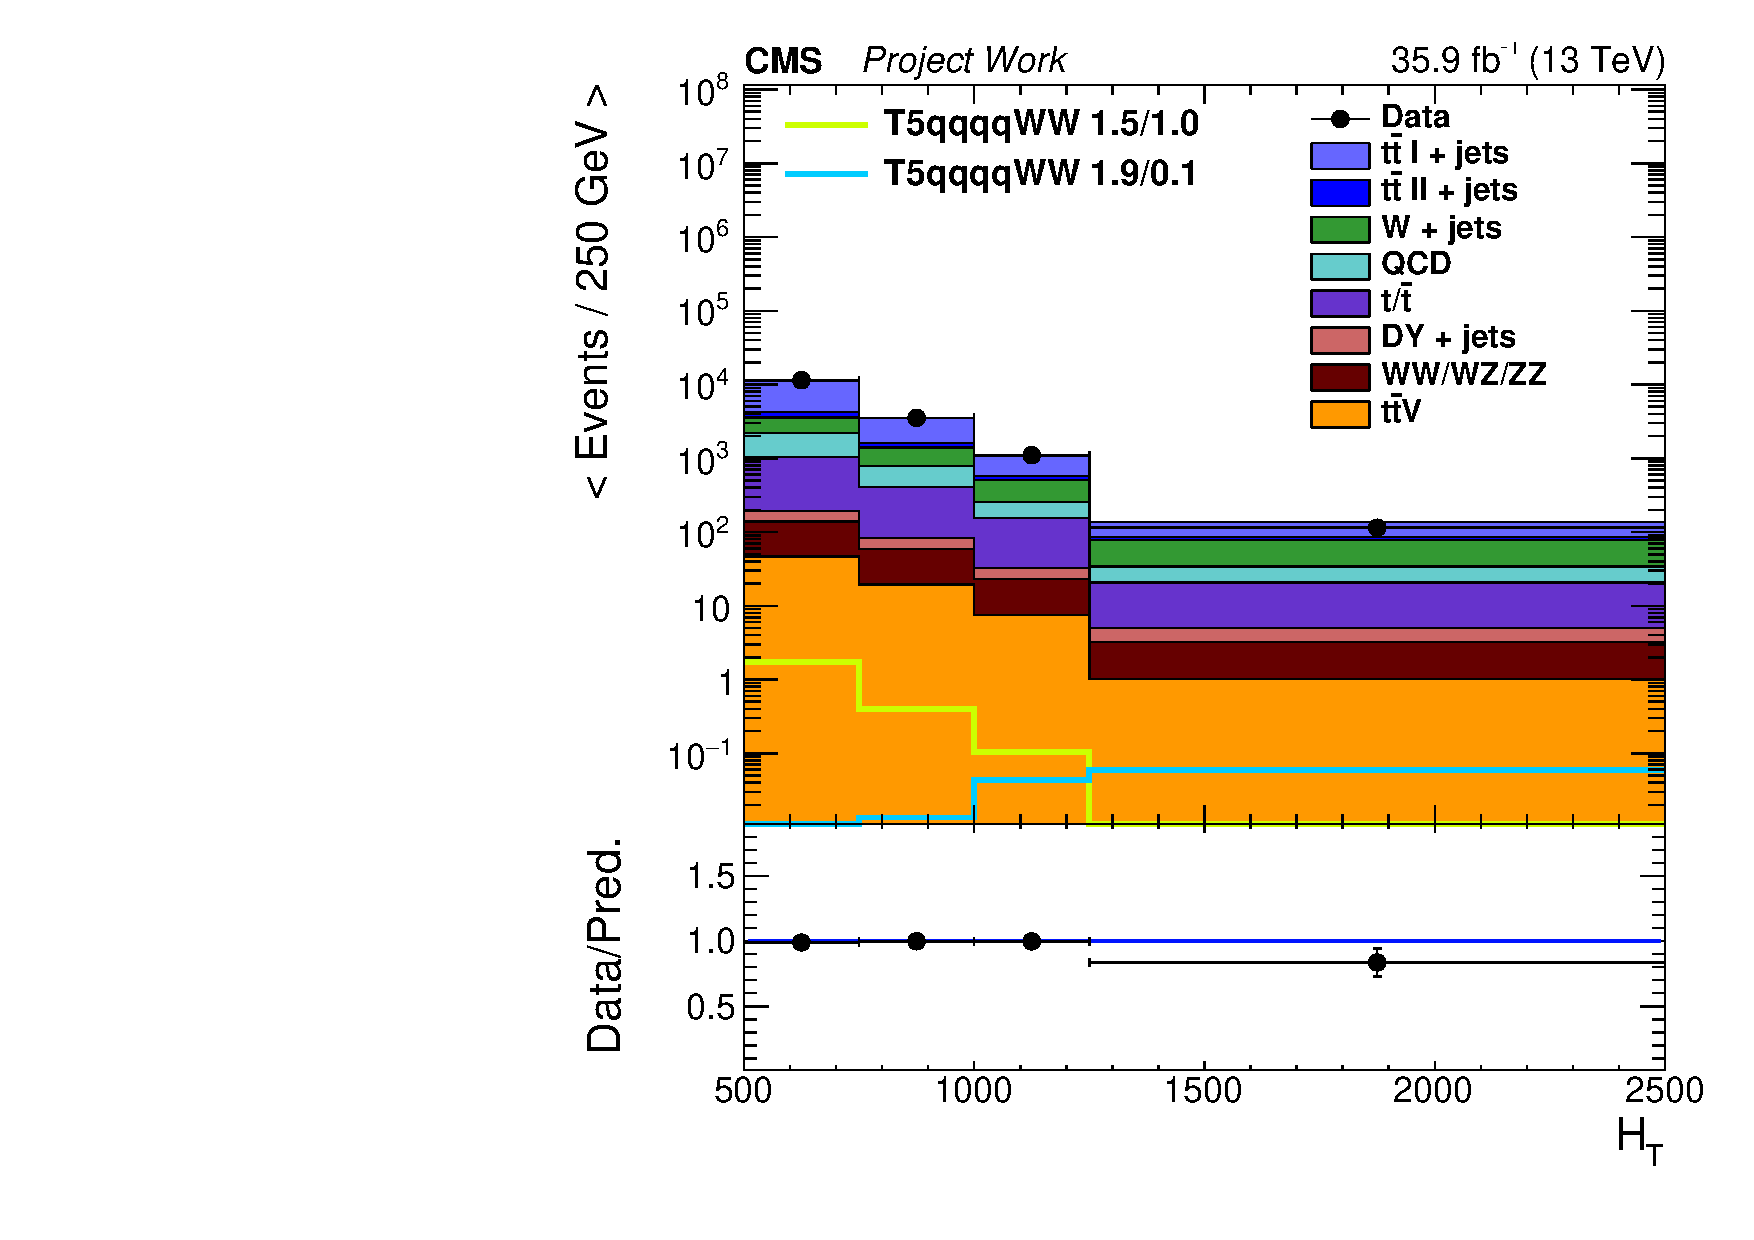
\includegraphics[angle=0,width=.32\textwidth]                    {Plots//analysis/control_Plots/ele/st250_ht500_njet4-5_nbtag1/htJet30jProject_Work.pdf}}
    \subfigure[\LT]{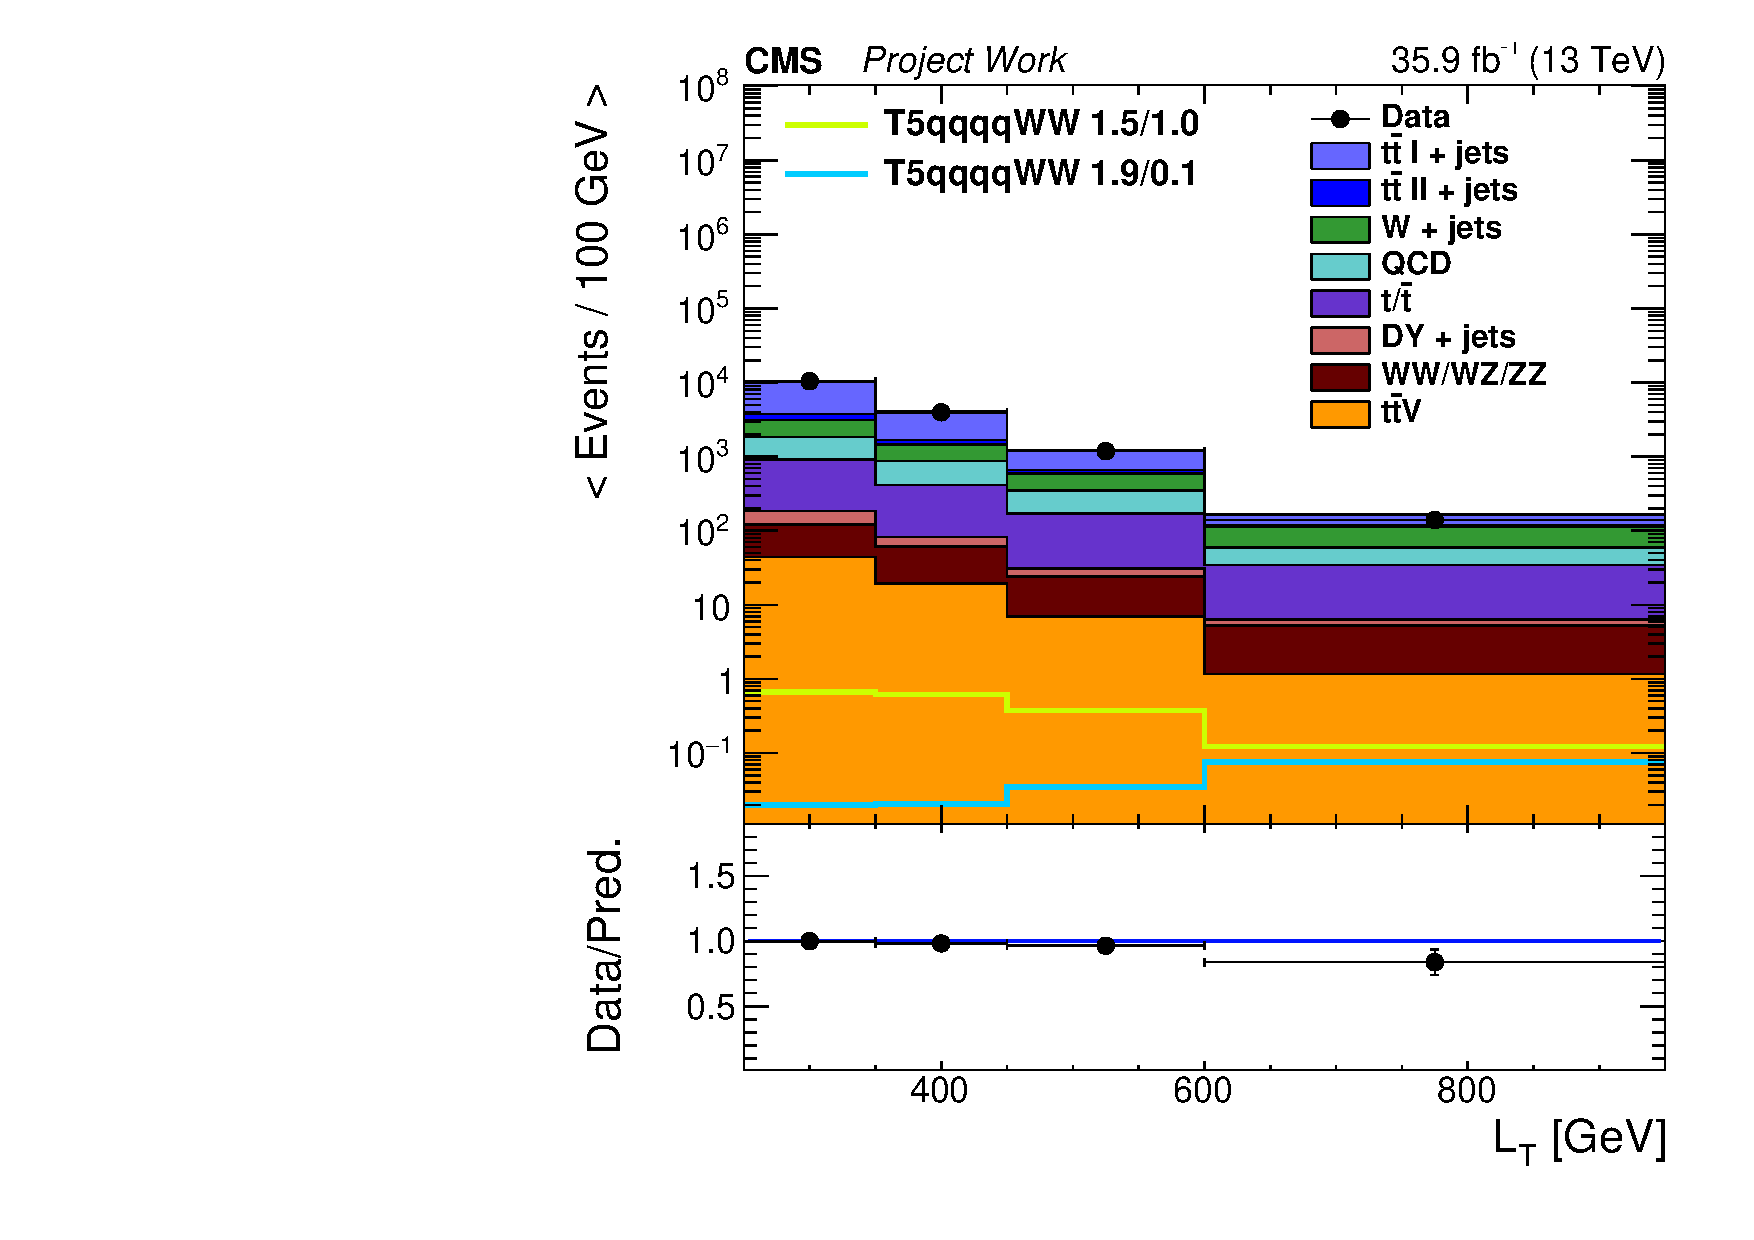
\includegraphics[angle=0,width=.32\textwidth]                    {Plots//analysis/control_Plots/ele/st250_ht500_njet4-5_nbtag1/LTProject_Work.pdf}}
    \subfigure[\DF]{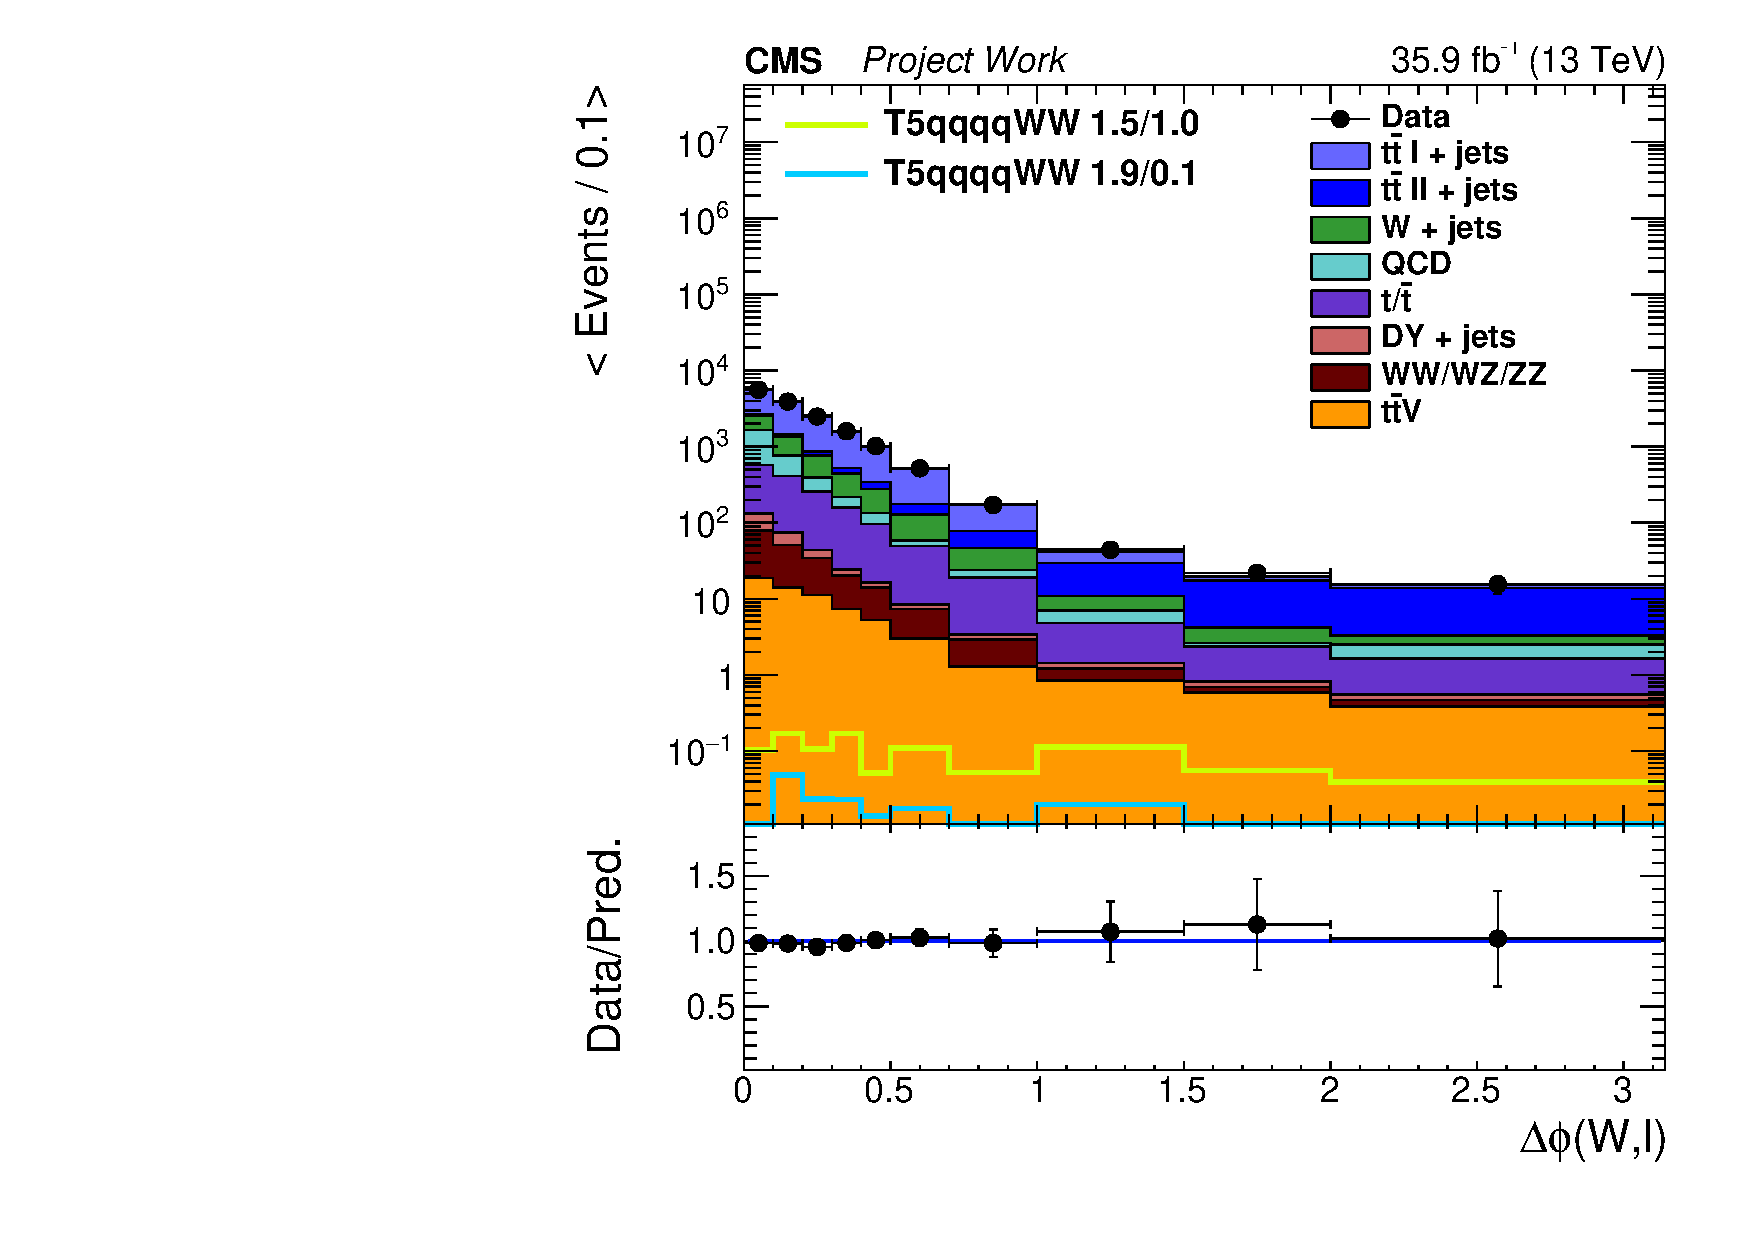
\includegraphics[angle=0,width=.32\textwidth]                    {Plots//analysis/control_Plots/ele/st250_ht500_njet4-5_nbtag1/deltaPhi_Wl_wideProject_Work.pdf}}

    \caption{Distribution of kinematic observables after requiring $\HT >$~500 \GeV, $\LT >$ 250~\GeV, $4\leq$ jets $\leq5$  and b-tagged jets (1 $e$ channel).
      %In order to blind the signal region, data events with large \DF (corresponding to the dynamic \DF cut) are excluded from the \DF plot.
    }
    \label{fig:0bele_1B_4_5jets_CR}
  \end{center}
\end{figure}

\begin{figure}[p]
  \begin{center}
    \subfigure[\njet]{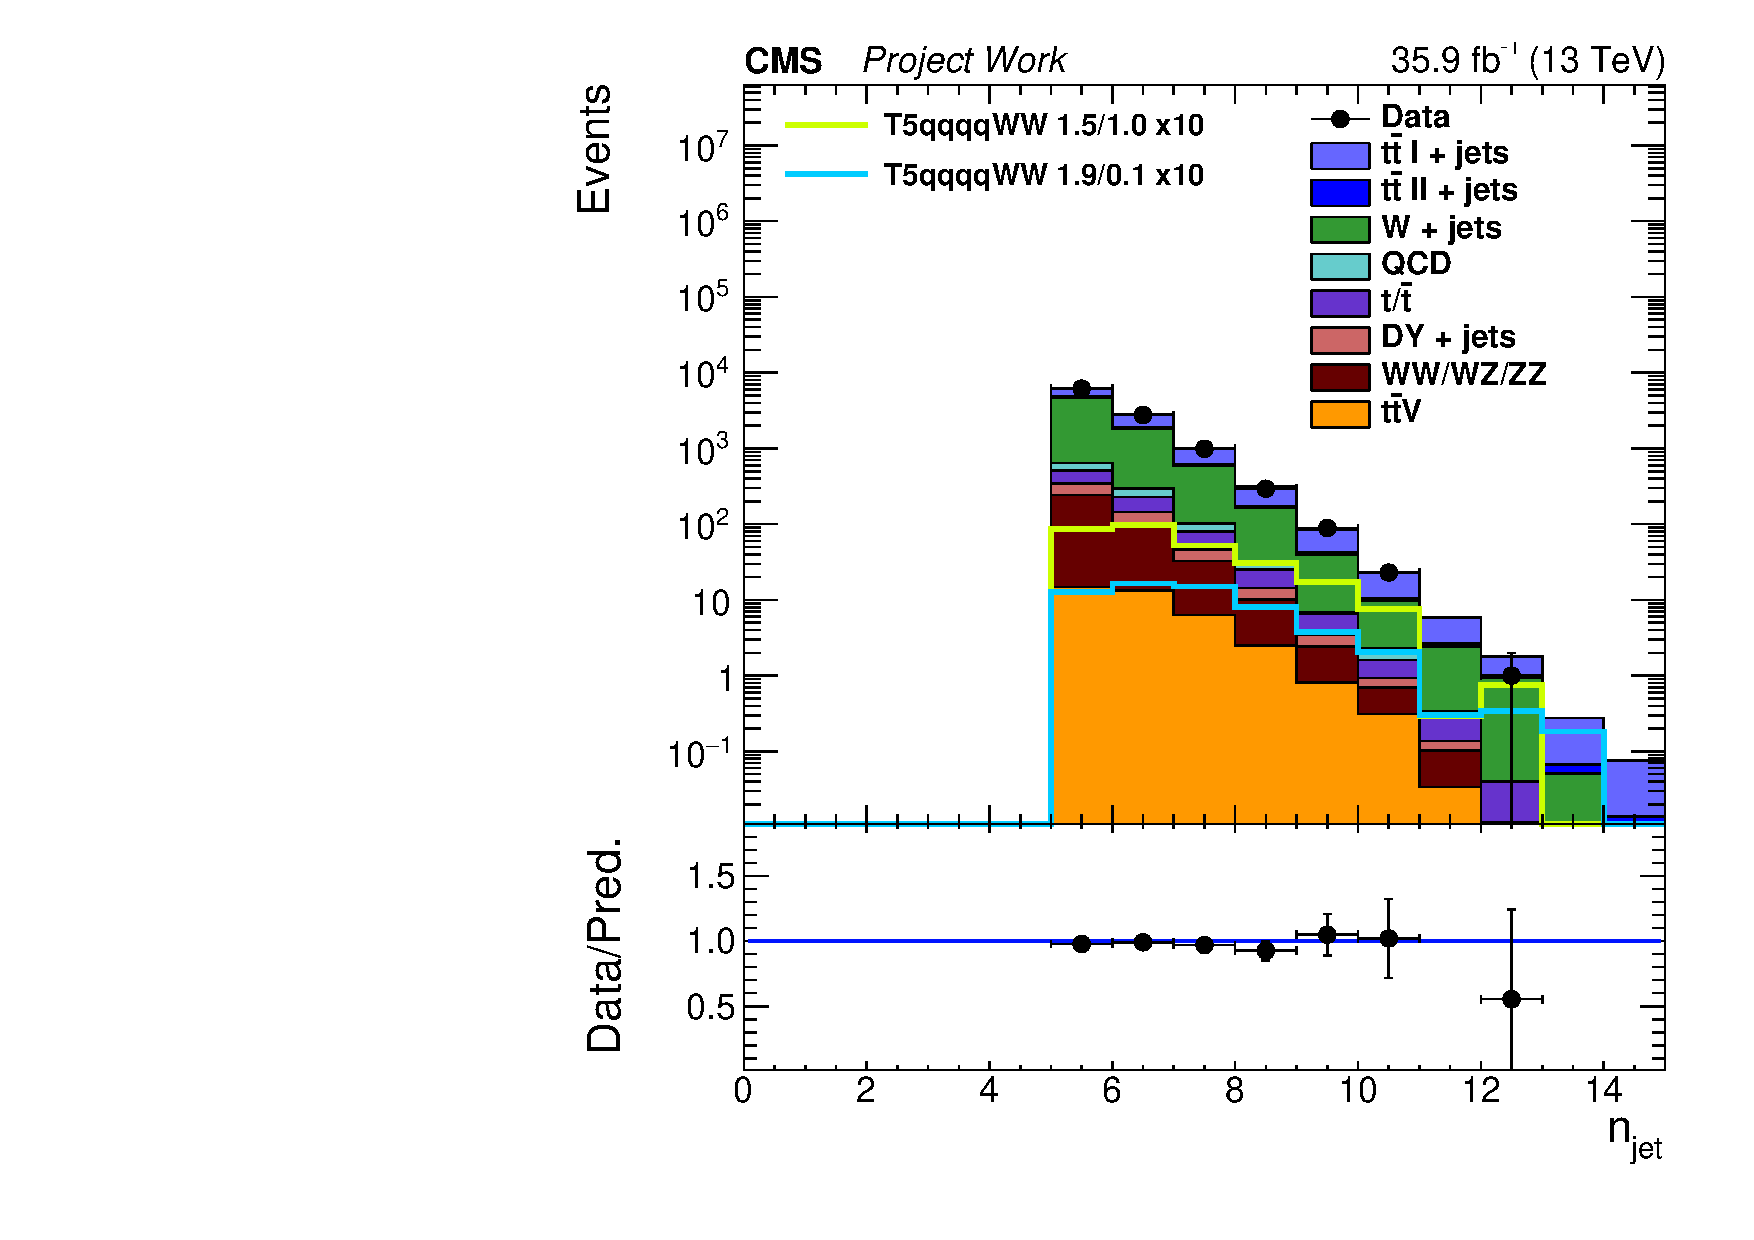
\includegraphics[angle=0,width=.32\textwidth]                  {Plots//analysis/control_Plots/mu/st250_ht500_njet5_nbtagEq0/nJet30Project_Work.pdf}}
    \subfigure[$p_T(\textrm{1st jet})$]{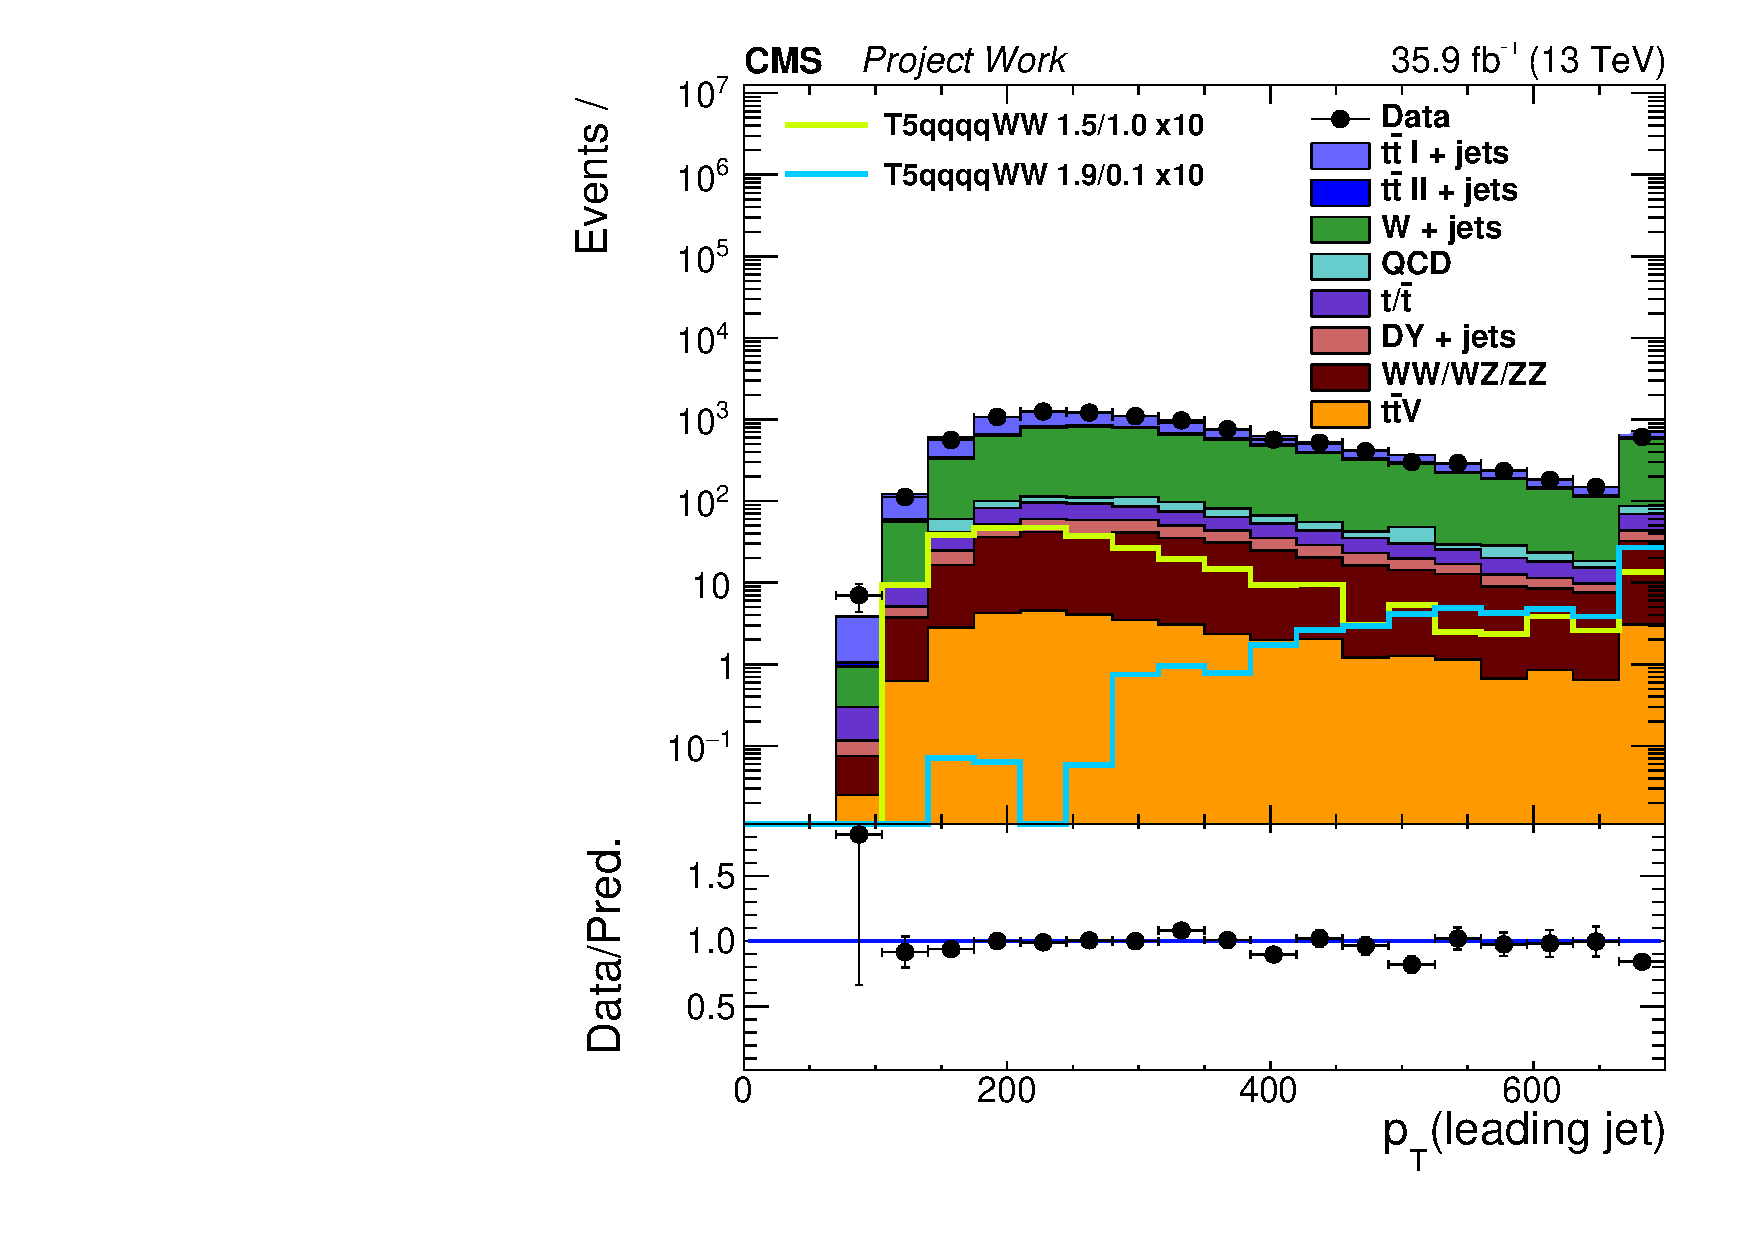
\includegraphics[angle=0,width=.32\textwidth]{Plots//analysis/control_Plots/mu/st250_ht500_njet5_nbtagEq0/leading_JetPtProject_Work.pdf}}
    \subfigure[$n_{\textrm{vertex}}$]{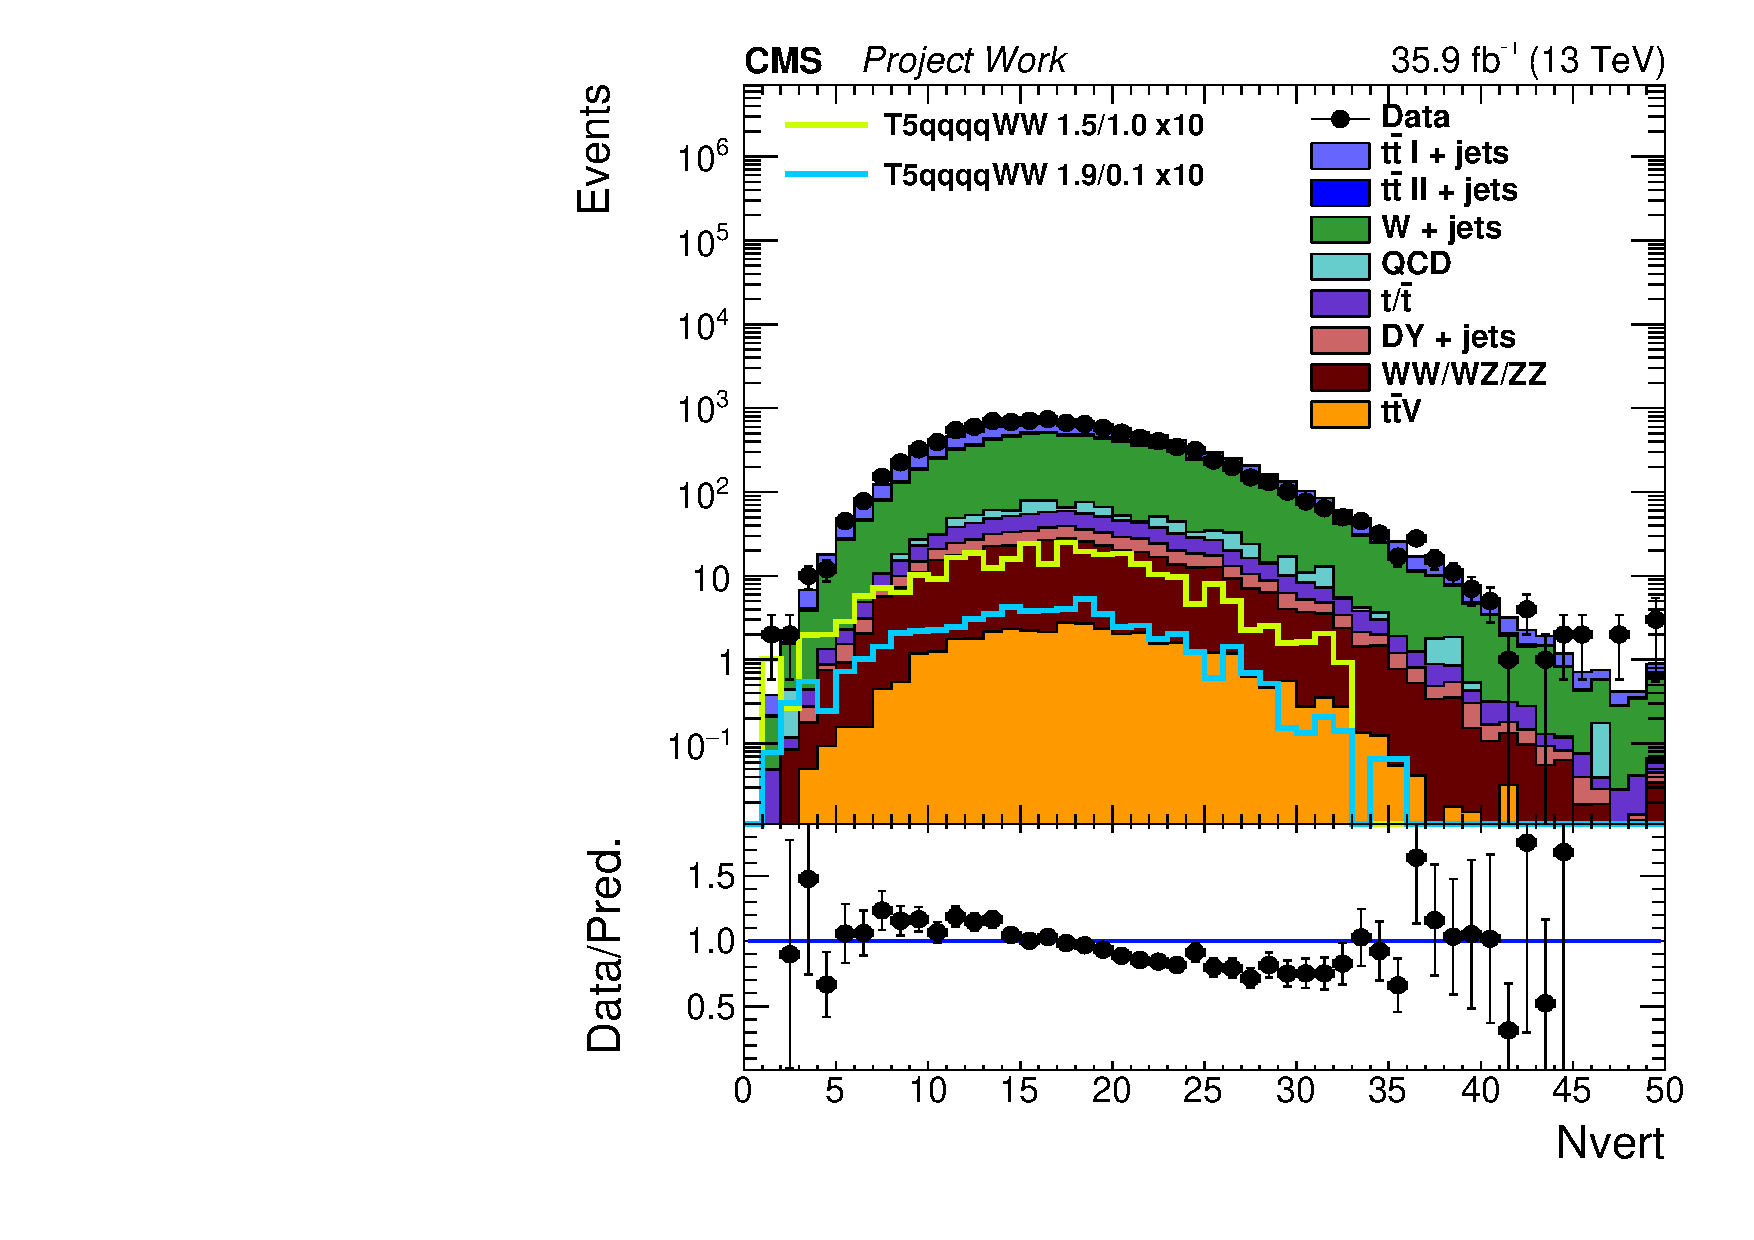
\includegraphics[angle=0,width=.32\textwidth]       {Plots//analysis/control_Plots/mu/st250_ht500_njet5_nbtagEq0/nVertProject_Work.pdf}}\\
    \subfigure[$p_T(l)$]{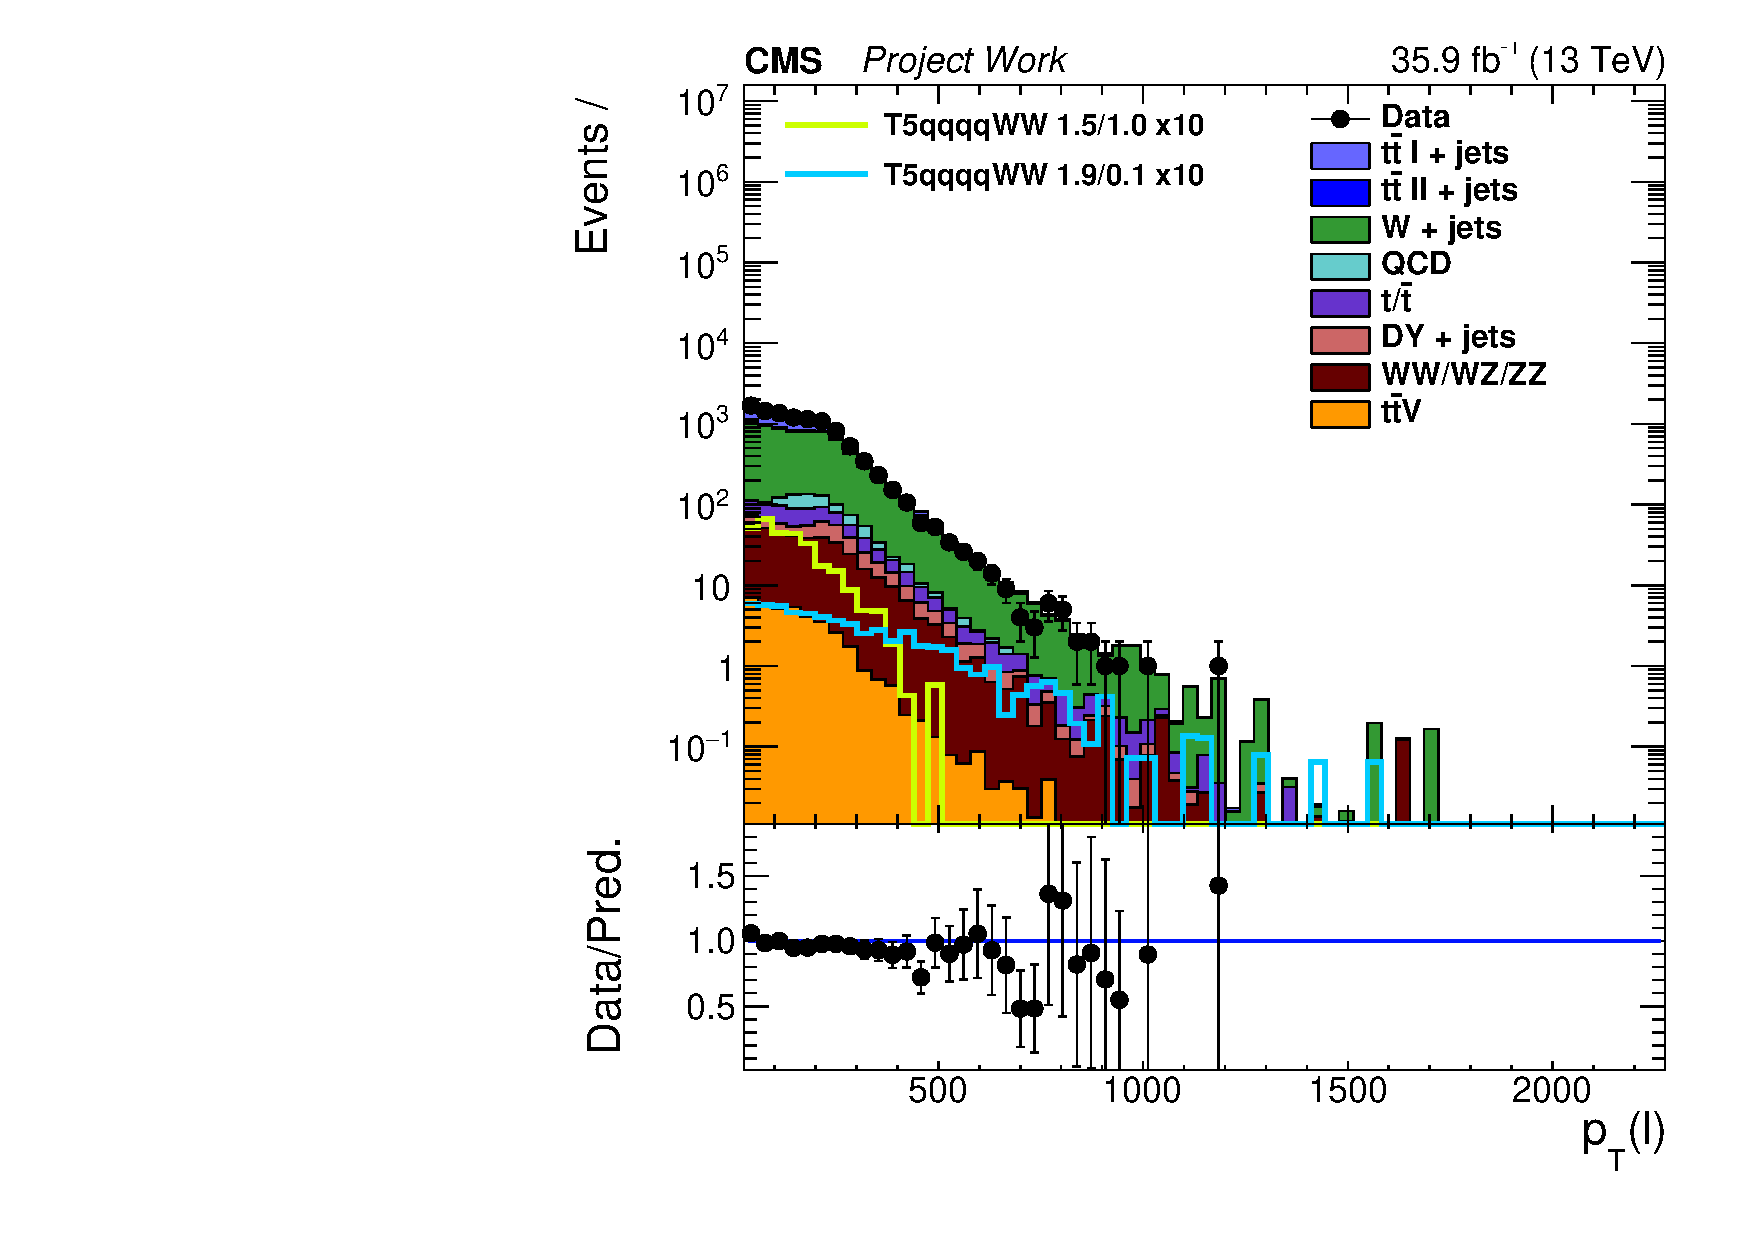
\includegraphics[angle=0,width=.32\textwidth]               {Plots//analysis/control_Plots/mu/st250_ht500_njet5_nbtagEq0/leptonPtProject_Work.pdf}}
    \subfigure[$m_{T2}$]{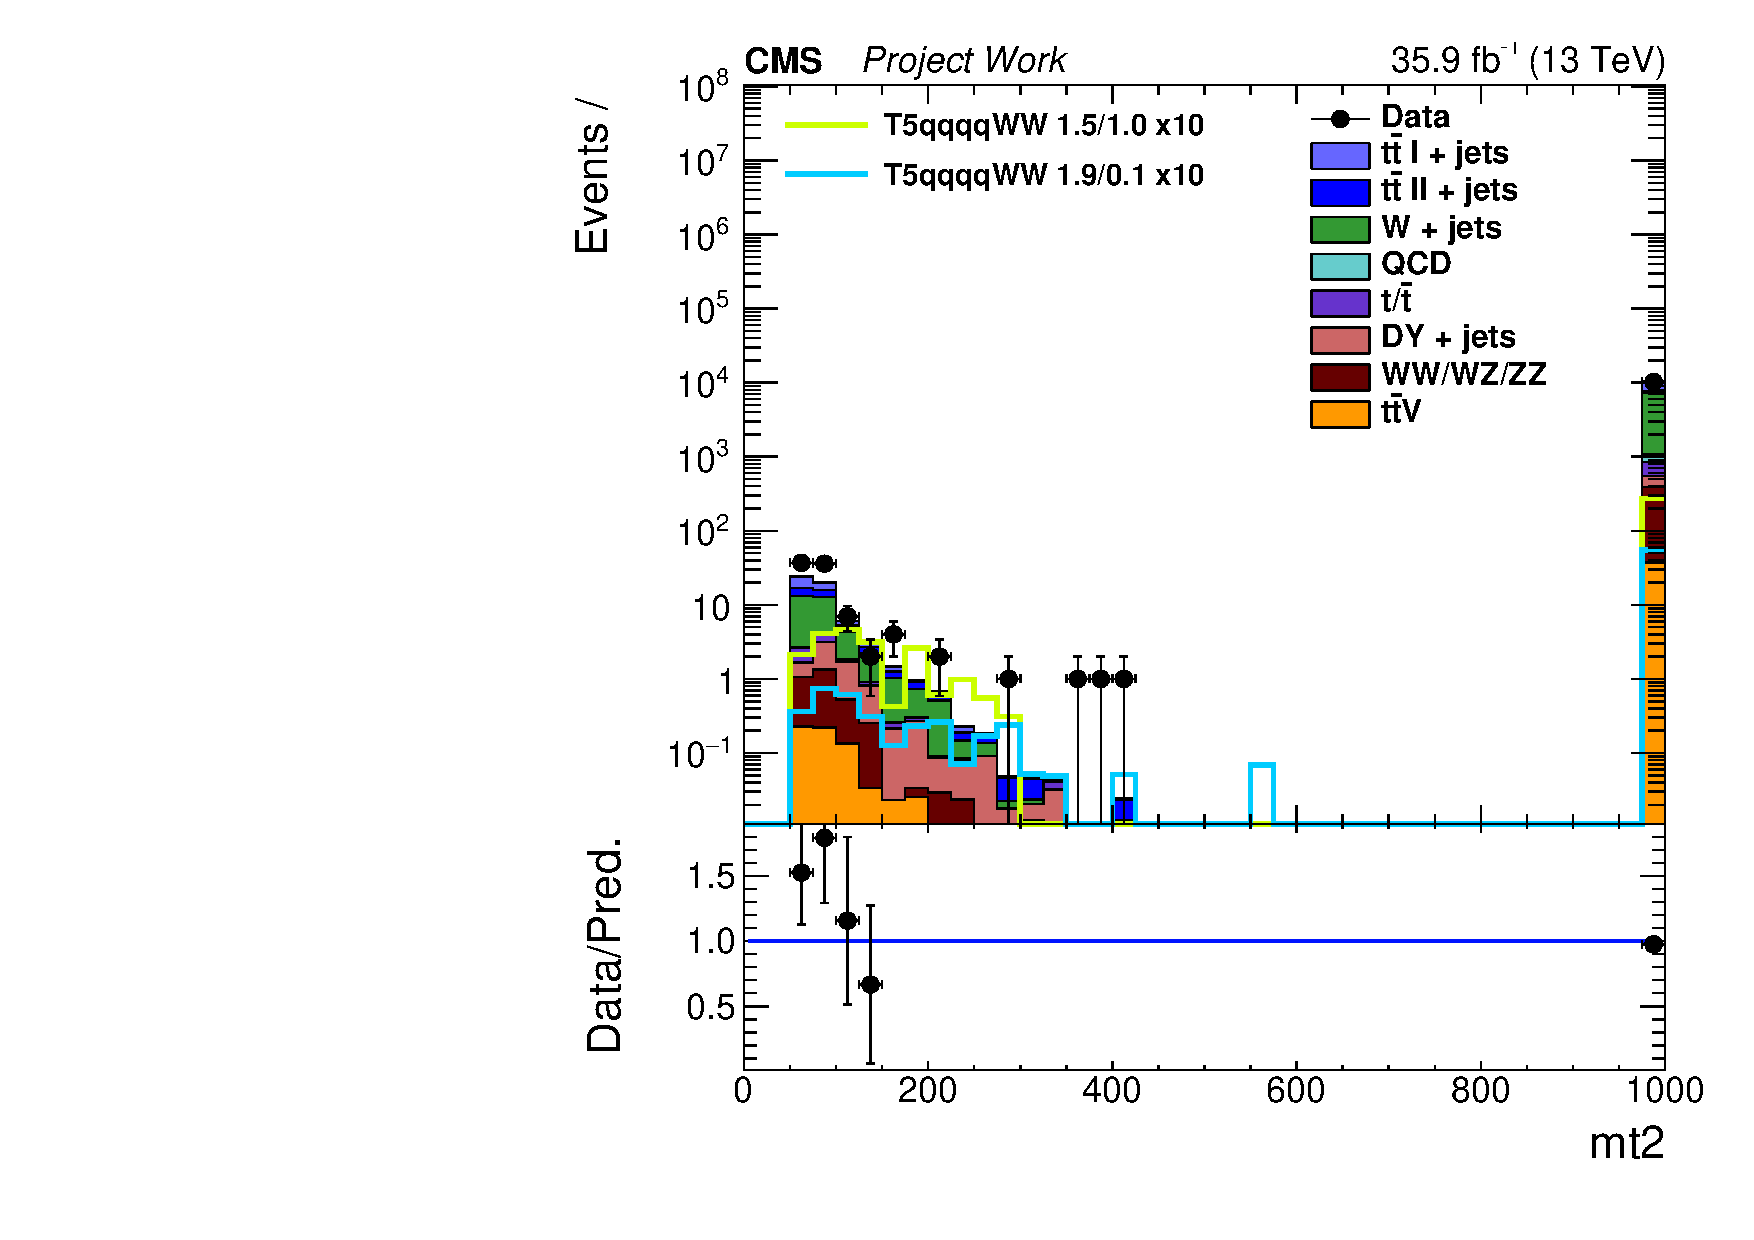
\includegraphics[angle=0,width=.32\textwidth]              {Plots//analysis/control_Plots/mu/st250_ht500_njet5_nbtagEq0/iso_MT2Project_Work.pdf}}
    \subfigure[miniIsolation$(l)$]{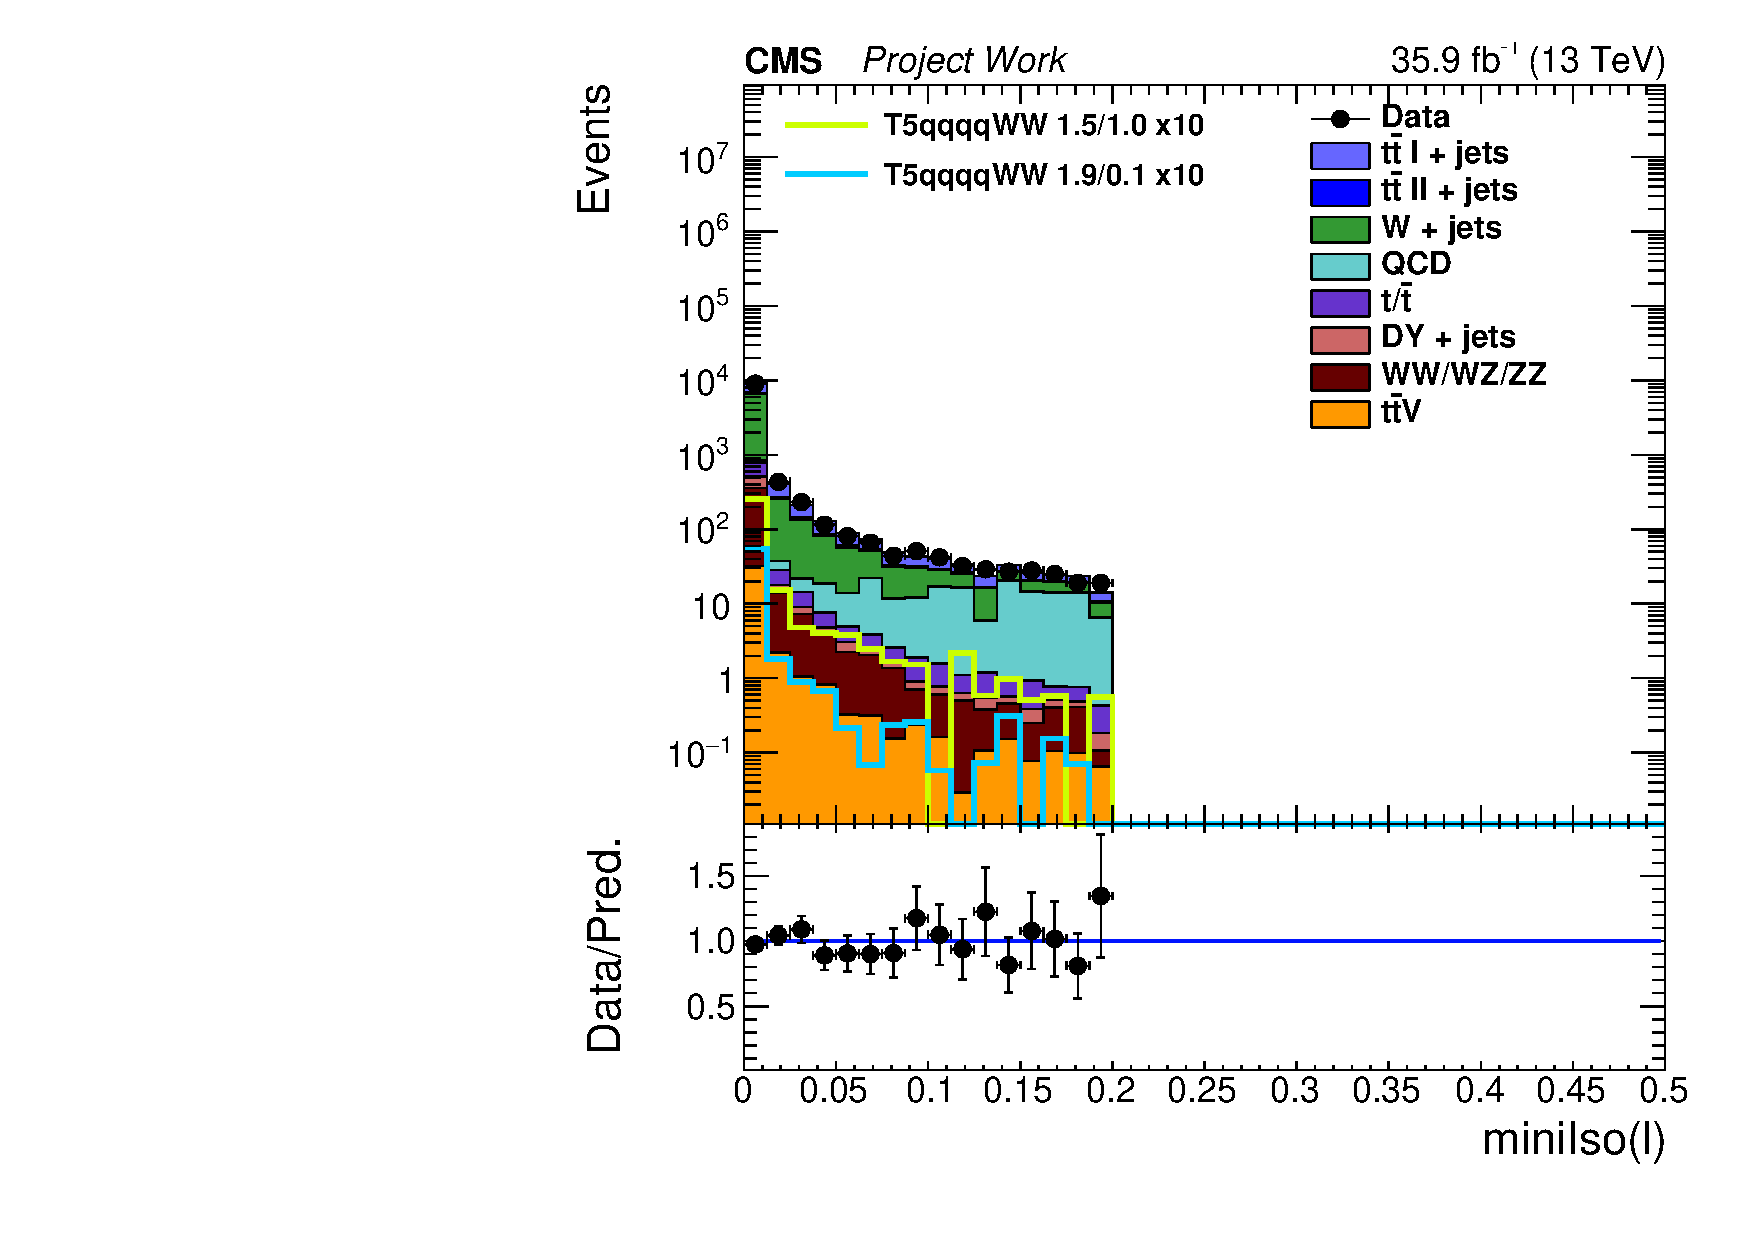
\includegraphics[angle=0,width=.32\textwidth]     {Plots//analysis/control_Plots/mu/st250_ht500_njet5_nbtagEq0/leptonminiIsoProject_Work.pdf}}\\
    \subfigure[\HT]{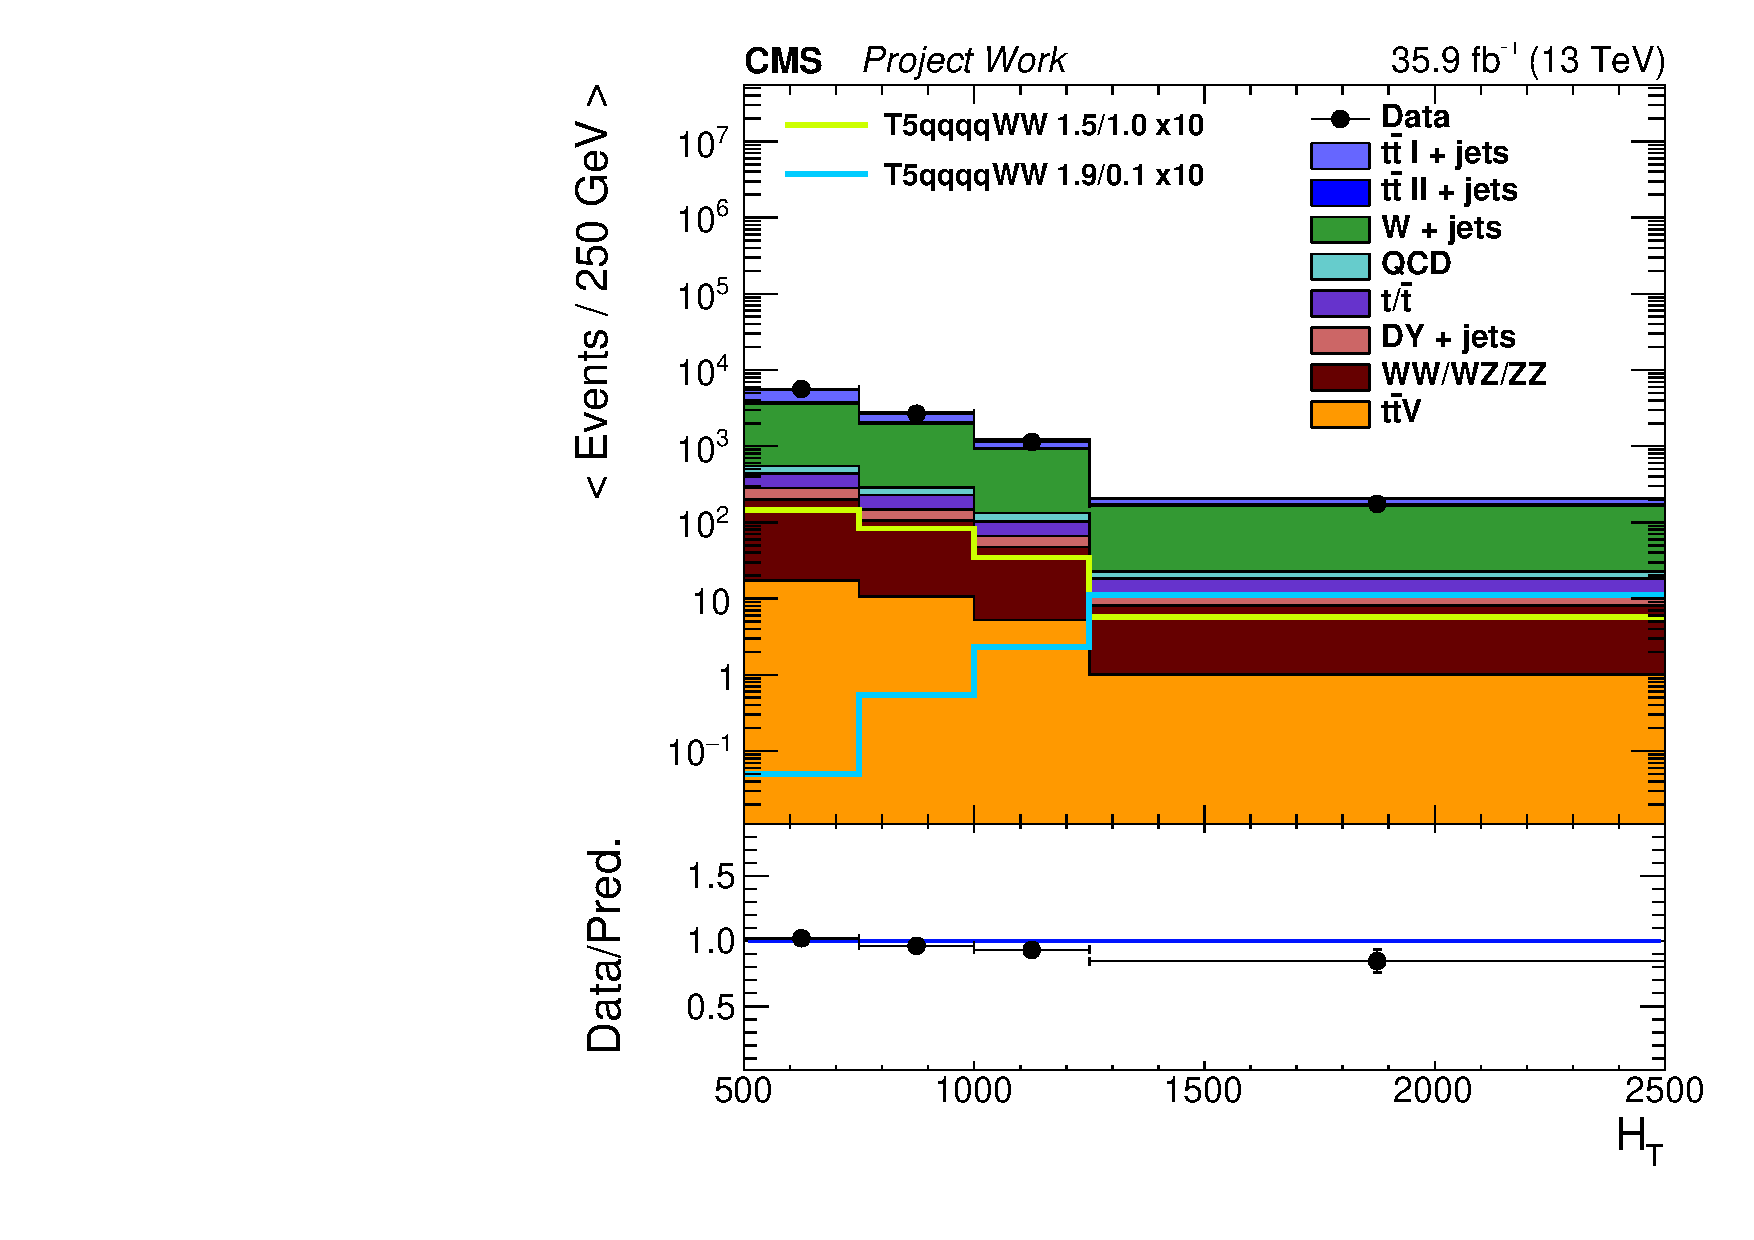
\includegraphics[angle=0,width=.32\textwidth]                    {Plots//analysis/control_Plots/mu/st250_ht500_njet5_nbtagEq0/htJet30jProject_Work.pdf}}
    \subfigure[\LT]{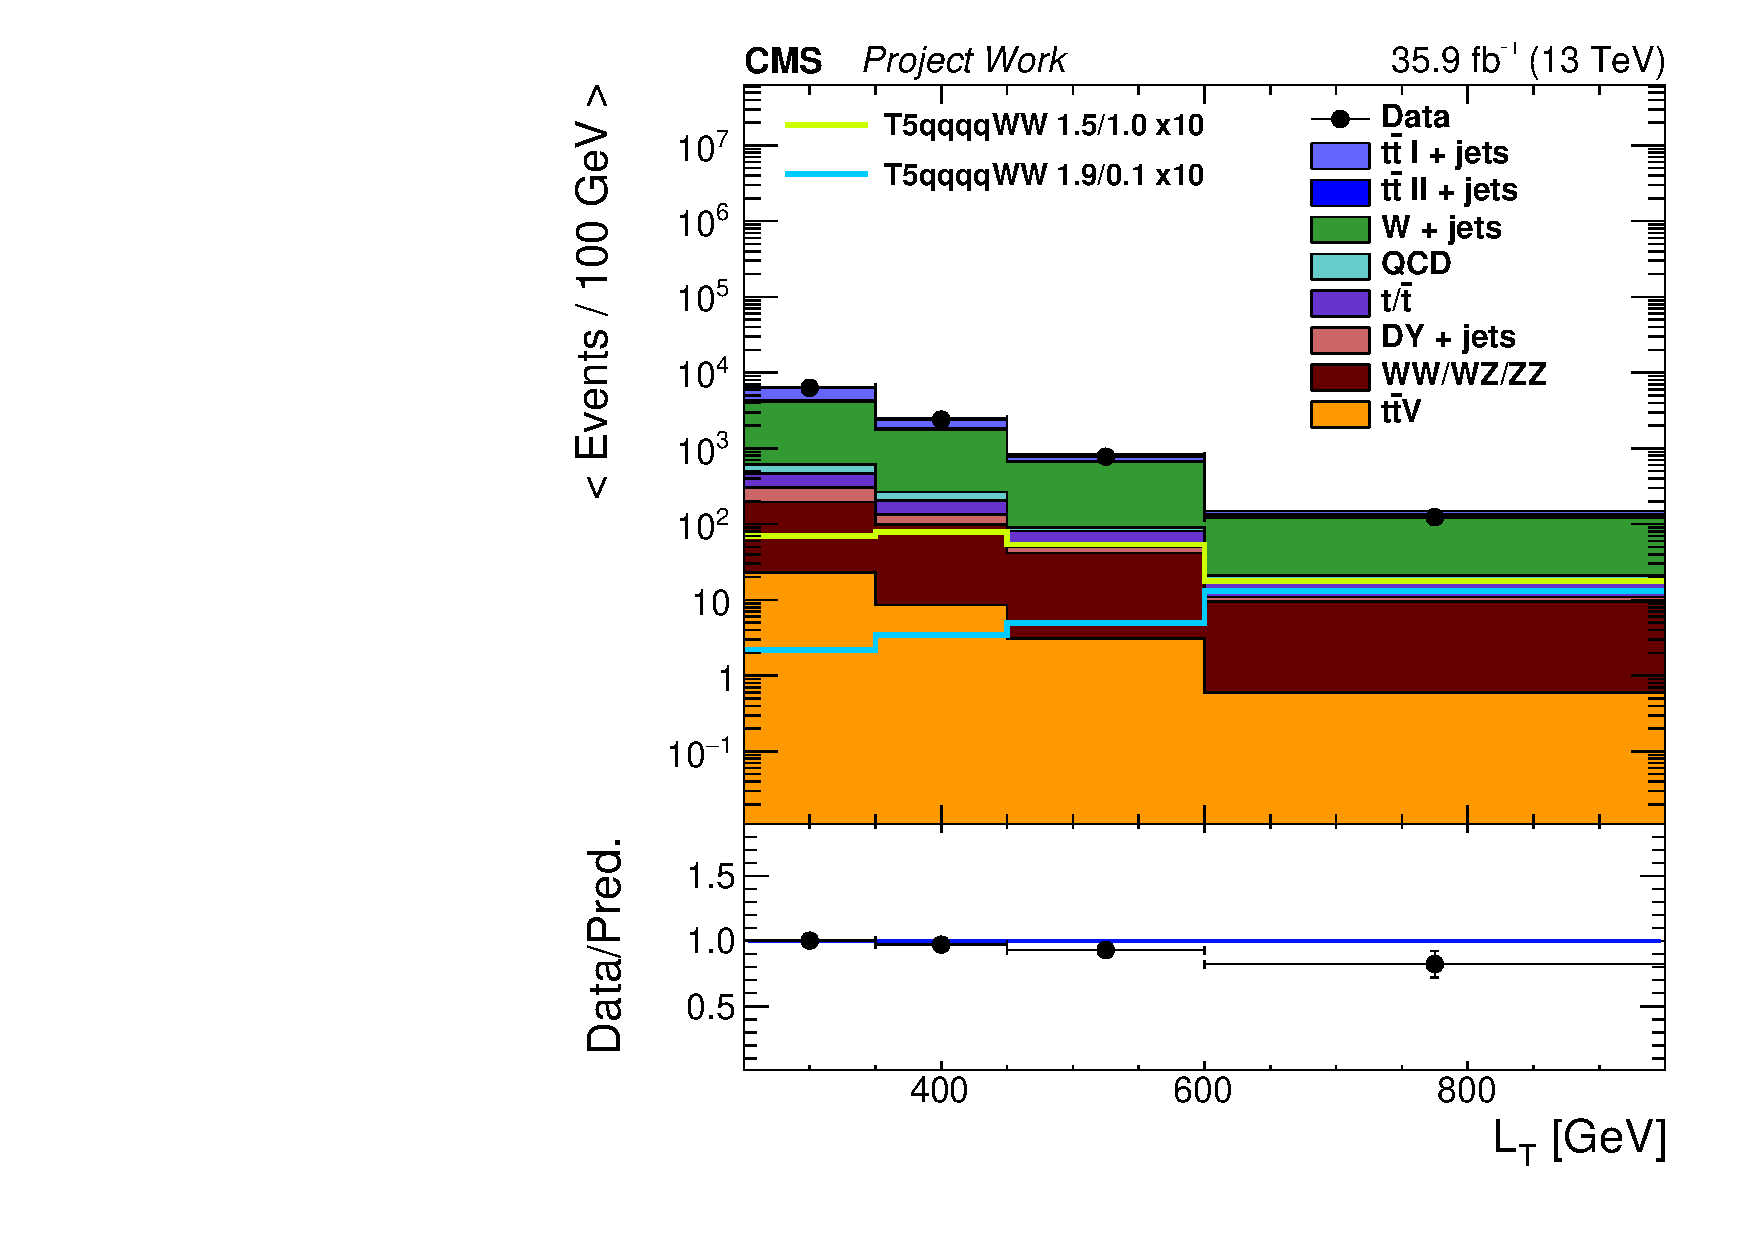
\includegraphics[angle=0,width=.32\textwidth]                    {Plots//analysis/control_Plots/mu/st250_ht500_njet5_nbtagEq0/LTProject_Work.pdf}}
    \subfigure[\DF]{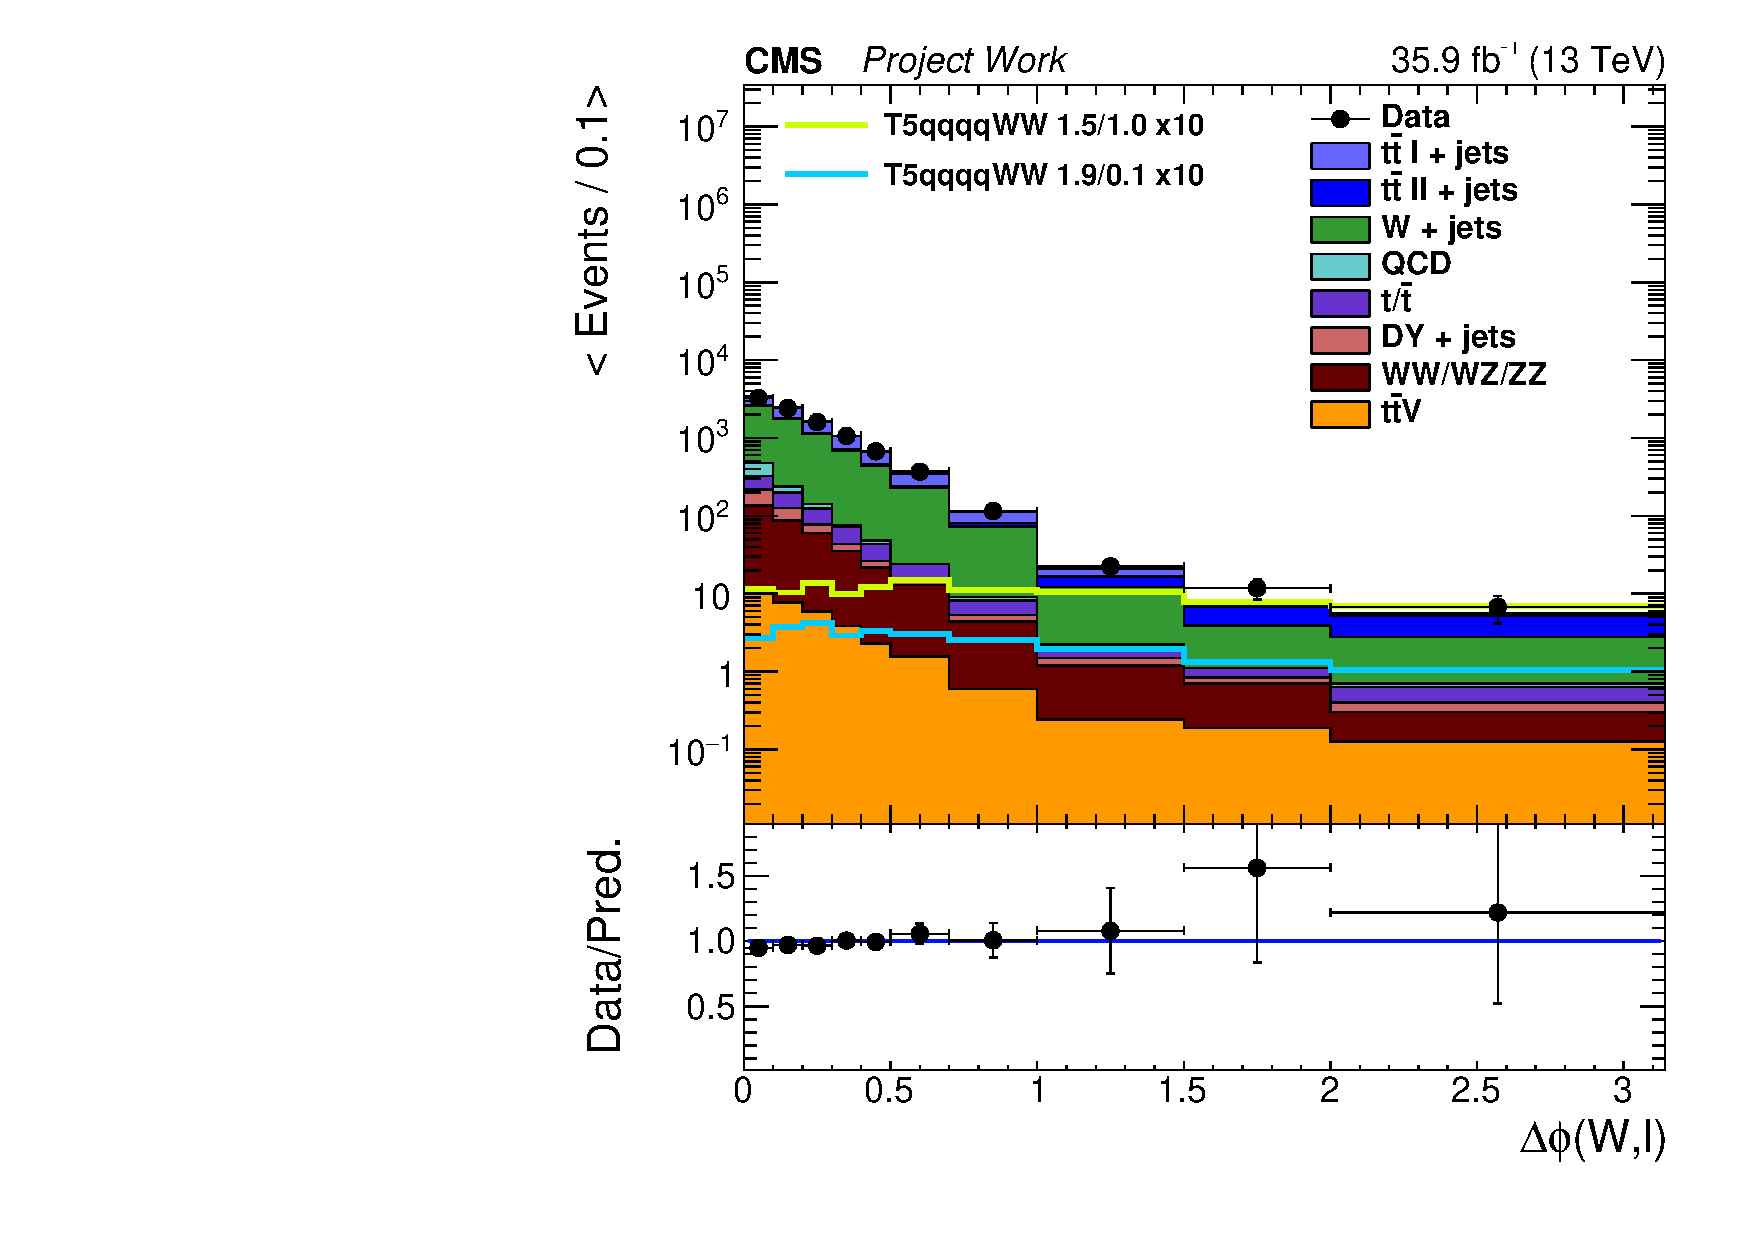
\includegraphics[angle=0,width=.32\textwidth]                    {Plots//analysis/control_Plots/mu/st250_ht500_njet5_nbtagEq0/deltaPhi_Wl_wideProject_Work.pdf}}
    \caption{Distribution of kinematic observables after requiring $\HT >$~500~\GeV, $\LT >$~250~\GeV, $\geq$ 5 jets and zero b-tagged jets (1 $\mu$ channel).
    }
    \label{fig:0bmu_0p5_CR}
  \end{center}
\end{figure}

\begin{figure}[p]
  \begin{center}
    \subfigure[\njet]{\includegraphics[angle=0,width=.32\textwidth]                  {Plots//analysis/control_Plots/ele/st250_ht500_njet5_nbtagEq0/nJet30Project_Work.pdf}}
    \subfigure[$p_T(\textrm{1st jet})$]{\includegraphics[angle=0,width=.32\textwidth]{Plots//analysis/control_Plots/ele/st250_ht500_njet5_nbtagEq0/leading_JetPtProject_Work.pdf}}
    \subfigure[$n_{\textrm{vertex}}$]{\includegraphics[angle=0,width=.32\textwidth]       {Plots//analysis/control_Plots/ele/st250_ht500_njet5_nbtagEq0/nVertProject_Work.pdf}}\\
    \subfigure[$p_T(l)$]{\includegraphics[angle=0,width=.32\textwidth]               {Plots//analysis/control_Plots/ele/st250_ht500_njet5_nbtagEq0/leptonPtProject_Work.pdf}}
    \subfigure[$m_{T2}$]{\includegraphics[angle=0,width=.32\textwidth]              {Plots//analysis/control_Plots/ele/st250_ht500_njet5_nbtagEq0/iso_MT2Project_Work.pdf}}
    \subfigure[miniIsolation$(l)$]{\includegraphics[angle=0,width=.32\textwidth]     {Plots//analysis/control_Plots/ele/st250_ht500_njet5_nbtagEq0/leptonminiIsoProject_Work.pdf}}\\
    \subfigure[\HT]{\includegraphics[angle=0,width=.32\textwidth]                    {Plots//analysis/control_Plots/ele/st250_ht500_njet5_nbtagEq0/htJet30jProject_Work.pdf}}
    \subfigure[\LT]{\includegraphics[angle=0,width=.32\textwidth]                    {Plots//analysis/control_Plots/ele/st250_ht500_njet5_nbtagEq0/LTProject_Work.pdf}}
    \subfigure[\DF]{\includegraphics[angle=0,width=.32\textwidth]                    {Plots//analysis/control_Plots/ele/st250_ht500_njet5_nbtagEq0/deltaPhi_Wl_wideProject_Work.pdf}}

    \caption{Distribution of kinematic observables after requiring $\HT >$~500~\GeV, $\LT >$~250~\GeV, $\geq$~5~jets and zero b-tagged jets (1 $e$ channel).
    }
    \label{fig:0bele_0p5_CR}
  \end{center}
\end{figure}
